%/////////////////////////////////////////////////////////////////////
%
% LaTeX definitions:     Ph.D. Dissertation
%                        Nuno Leite
%                        september 2015
%
%/////////////////////////////////////////////////////////////////////


\documentclass[12pt, a4paper, openright, twoside]{report}

\usepackage{listings}
\usepackage{color}

\definecolor{dkgreen}{rgb}{0,0.6,0}
\definecolor{gray}{rgb}{0.5,0.5,0.5}
\definecolor{mauve}{rgb}{0.58,0,0.82}

\lstset{frame=tb,
  language=Java,
  aboveskip=3mm,
  belowskip=3mm,
  showstringspaces=false,
  columns=flexible,
  basicstyle={\small\ttfamily},
  numbers=none,
  numberstyle=\tiny\color{gray},
  keywordstyle=\color{blue},
  commentstyle=\color{dkgreen},
  stringstyle=\color{mauve},
  breaklines=true,
  breakatwhitespace=true,
  tabsize=3
}

%//to enable Code listings

%////////////
% Acronyms
% Load the package with the acronym option. Omit the dot at the end of each description
\usepackage[acronym,nomain,toc,nopostdot]{glossaries}
% Suppress acronym bold font
\renewcommand*{\glsnamefont}[1]{\textmd{#1}}

% For resetting acronyms at the beginning of each chapter
\usepackage{etoolbox}
\preto\chapter\glsresetall

%
\usepackage{glossaries-extra}
\renewcommand{\glsfirstlongdefaultfont}[1]{\emph{#1}}
\setabbreviationstyle[acronym]{long-short}
%

% Redefining indentation in the List of acronyms
\newglossarystyle{super3colleft}{%
  \renewenvironment{theglossary}%
    {\tablehead{}\tabletail{}%
     \begin{supertabular}{@{}>{\bfseries}lp{\glsdescwidth}p{\glspagelistwidth}}}%
    {\end{supertabular}}%
  \renewcommand*{\glossaryheader}{}%
  \renewcommand*{\glsgroupheading}[1]{}%
  \renewcommand*{\glossaryentryfield}[5]{%
    \glsentryitem{##1}\glstarget{##1}{##2} & ##3 & ##5\\}%
  \renewcommand*{\glossarysubentryfield}[6]{%
     &
     \glssubentryitem{##2}%
     \glstarget{##2}{\strut}##4 & ##6\\}%
  \renewcommand*{\glsgroupskip}{ & &\\}%
}



\newlength{\acronymlabelwidth}
\setlength{\acronymlabelwidth}{0.25\textwidth}
%////////////

% Chapter style
\usepackage[Lenny]{fncychap}

% Chapter minitoc
\usepackage{minitoc}

% English language
\usepackage[english]{babel}
\usepackage[T1]{fontenc}
%\usepackage[latin1]{inputenc}
\usepackage[utf8]{inputenc}

% Times New Roman typeface
%\usepackage{textcomp}
\renewcommand{\rmdefault}{ptm} % set Times as the default text font
% If AMS-LaTeX is used, it can be loaded before or after mtpro2
\usepackage{amsmath}		
%% The following loads mtpro and defines some common MTPro options 
%\usepackage[subscriptcorrection, slantedGreek, nofontinfo]{mtpro2}

% My styles
\usepackage{myStyles}


% Graphics package
%\usepackage[dvips]{graphicx}
\usepackage{graphicx}

% Other packages
\usepackage{epsfig}
\usepackage[nottoc]{tocbibind} % To include bibliography in TOC
\usepackage{latexsym}
% Fancy headers
\usepackage{fancyhdr}




%////////////// ADDED PACKAGES //////////////////
%\usepackage{natbib,hyperref} % For numerical format
\usepackage[natbibapa]{apacite} % For APA format
\usepackage{hyperref}
\usepackage{graphics} % resizebox command
\usepackage[toc,page]{appendix} % For defining appendices
\PassOptionsToPackage{hyphens}{url} % For processing correctly underscores in URL
\usepackage{subfigure}
\usepackage{calc}
%\usepackage{amssymb} % MTPro2 fonts contain all of the symbols provided by amssymb. 
% The amsthm package provides extended theorem environments
% \usepackage{amsthm}
\usepackage{amstext}
\usepackage{amsmath}
\usepackage{textcomp} % degree symbol 
\usepackage{graphicx}
%///
% Algorithm package
\usepackage[chapter]{algorithm}
%\usepackage{algorithmicx}
\usepackage{algpseudocode} % Typesetting using the algorithmicx package
% Algorithm numbering
\renewcommand{\thealgorithm}{\arabic{chapter}.\arabic{algorithm}} 
%///

\usepackage{lineno} % linenomath

% Allow break in align math environment
\allowdisplaybreaks

\usepackage{eqparbox,array}

\newcommand\LONGCOMMENT[1]{%
	\hfill$\triangleright$ \begin{minipage}[t]{15\eqboxwidth{algorithmiccomment}}#1\strut\end{minipage}%
}

\newcommand\LONGCOMMENTONE[1]{%
	\hfill$\triangleright$ \begin{minipage}[t]{14\eqboxwidth{algorithmiccomment}}#1\strut\end{minipage}%
}

\newcommand\LONGCOMMENTTWO[1]{%
	\hfill$\triangleright$ \begin{minipage}[t]{17\eqboxwidth{algorithmiccomment}}#1\strut\end{minipage}%
}

% For floating point columns
\usepackage{etoolbox} 
\usepackage[tight-spacing=true]{siunitx}
\robustify\bfseries
% For bold cells using siunitx
\newcommand{\be}[2]{%
	\multicolumn{1}{S[table-format=#1,
		mode=text,
		text-rm=\fontseries{b}\selectfont
		]}{#2}}

% For bold cells using siunitx
\newcommand{\beIt}[2]{%
	\multicolumn{1}{S[table-format=#1,
		mode=text,
		text-rm=\fontseries{b}\fontshape{it}\selectfont
		]}{#2}}

% For bold cells using siunitx
\newcommand{\beSci}[1]{%
	\multicolumn{1}{
		S[table-format =1.2e4,%    
%		S[exponent-product = \cdot,
%		round-mode = figures,
%		round-precision = 3,
		detect-weight=true, 
		detect-family=true,
		mode=text,
		text-rm=\fontseries{b}\selectfont
		]}{#1}}

%\usepackage[tight-spacing=true]{siunitx}

\usepackage{booktabs} % Professional tables
% Use in coloured tables
\usepackage{cancel}
\usepackage[pdftex, table]{xcolor}  % Coloured text etc.
%To tweak the space between columns (LaTeX will by default choose very tight columns), one can alter the column separation: \setlength{\tabcolsep}{5pt}. The default value is 6pt.
\setlength{\tabcolsep}{5pt}
%\setlength{\tabcolsep}{1.7pt}
\usepackage{todonotes}
\usepackage{multirow}
\usepackage{pdflscape}
\usepackage{enumerate}
\usepackage{stfloats} % TA plots
\usepackage{adjustbox}
\usepackage{longtable} % For long tables spanning multiple pages

% For removing underfull \hbox warning in the bibliography
\apptocmd{\sloppy}{\hbadness 10000\relax}{}{}
% Alternatively
%\usepackage{etoolbox}
%\apptocmd{\thebibliography}{\raggedright}{}{}

\usepackage{float}
\floatstyle{plaintop}
\restylefloat{table}

%\newcommandx{\info}[2][1=]{\todo[linecolor=OliveGreen,backgroundcolor=OliveGreen!25,bordercolor=OliveGreen,#1]{#2}}

\newif\ifboldnumber
\newcommand{\boldnext}{\global\boldnumbertrue}

% Default definition is \footnotesize#1:
\algrenewcommand\alglinenumber[1]{%
	\footnotesize\ifboldnumber\bfseries\fi\global\boldnumberfalse#1:}

\usepackage{verbatimbox}

\newcolumntype{L}[1]{>{\raggedright\let\newline\\\arraybackslash\hspace{0pt}}m{#1}}


\usepackage{doi}
\renewcommand\doitext{} % Remove duplicate "doi:" prefix
% For placing figures and tables in the next page
\usepackage{afterpage}
\usepackage{flafter}
% siunitx EN language floating point separator
\sisetup{group-separator = {,}}

% For reducing \hbox warnings
\sloppy

%////////////////////////////////////////////////


\usepackage{setspace}
\onehalfspacing % or \doublespacing

% Line spacing
%\linespread{1.25} %// LAST
%\linespread{1.35}
%\linespread{1.4}

% Page dimensions - equivalent to 15 cm x 23 cm
\usepackage[left=3.5cm,right=2.5cm,top=3cm,bottom=3.7cm]{geometry}

%\usepackage[headheight=14pt, text={15cm,23cm}, twoside, bindingoffset=1cm]{geometry}

%\usepackage[headheight=14pt, text={15cm,23cm}, top=2cm, left=2.5cm, right=2.5cm, bottom=2.5cm, twoside, bindingoffset=1cm, includefoot, includehead]{geometry}

% Page dimensions
%\pagestyle{plain}
%\setlength{\oddsidemargin}{0.5cm} 
%\setlength{\evensidemargin}{-0.5cm}
%\setlength{\topmargin}{-1cm} 
%\setlength{\textheight}{23cm}
%\setlength{\textwidth}{16cm}
%



%-
% //////// Changing default figure captions ///////
%-
%\setlength{\abovecaptionskip}{10pt}
\setlength{\belowcaptionskip}{5px}


%\makeatletter % Allow the use of @ in command names
%\long\def\@makecaption#1#2{%
%\vskip\abovecaptionskip
%\sbox\@tempboxa{ \textbf{#1} \hspace{0.5em} #2}%
%\ifdim \wd\@tempboxa >\hsize
%{ \textbf{#1} \hspace{0.5em}  #2\par}
%\else
%\hbox to\hsize{\hfil\box\@tempboxa\hfil}%
%\fi
%\vskip\belowcaptionskip}
%\makeatother % Cancel the effect of \makeatletter 
%% ////////////////////////////
%
%% //// Use 'Computer Modern' typewriter font, not 'Lucida Typewriter' ////
%\renewcommand{\ttdefault}{cmtt}%
%% //// Estilo adoptado para trocos de codigo no texto ////
%\newcommand{\code}[1]{{\tt #1}}



% ///// Fancy headers ////////
\usepackage{fancyhdr}
\pagestyle{fancy}
\fancyhf{}

\renewcommand{\chaptermark}[1]{%
  \markboth{\chaptername \ \thechapter \hspace{0.5em} \emph{#1}}{}}

\renewcommand{\sectionmark}[1]{%
  \markright{\thesection \hspace{0.5em} #1}{}}
     
\renewcommand{\headrulewidth}{0pt}

\fancypagestyle{plain}{%
\fancyhf{} % clear all header and footer fields
\fancyfoot[C]{\small\thepage} % except the center
\renewcommand{\headrulewidth}{0pt}
\renewcommand{\footrulewidth}{0pt}}
% /////////////////////////////////


% Load acronym definitions
\loadglsentries[\acronymtype]{Acronyms/Acronyms}

% Generate the glossary
\makeglossaries


\usepackage{silence}

\WarningFilter{minitoc(hints)}{W0023}
\WarningFilter{minitoc(hints)}{W0028}
\WarningFilter{minitoc(hints)}{W0030}

\WarningFilter{blindtext}{} % this takes care of the `blindtext` messages




%//////////////////////////
%
% Main matter
%
%//////////////////////////
\begin{document}

% Environment for displaying examples
%\theoremstyle{definition}
\newtheorem{exmp}{Example}[section]


% Commands
\renewcommand\bibname{References}


% Document cover
\thispagestyle{empty}

\begin{figure}[ht!]
	%\vspace*{-4cm}
	\centering
	\scalebox{0.6}{
\includegraphics{FrontCover/Logo_ISEL}}
\end{figure}


\centerline{\Large\textbf{INSTITUTO POLIT\'{E}CNICO DE LISBOA}}
\bigskip
%\bigskip
\centerline{\Large\textbf{INSTITUTO SUPERIOR DE ENGENHARIA DE LISBOA}}


\bigskip
\bigskip

\title{{\large Licenciatura em Engenharia de Inform\'{a}tica e de Computadores}}

\bigskip
\bigskip

\begin{center}

 
{\LARGE \textbf{PostChat}}

\bigskip
{\Large \textbf{"Bring Back Postcards"}}

\bigskip
\bigskip
\bigskip
\bigskip
\bigskip
\bigskip
\bigskip
\bigskip



{\Large \textbf{\vspace*{1em}Ant\'{o}nio Carvalho n.\textdegree $\ $48347}}

{\Large \textbf{e-mail: \texttt{a48347@alunos.isel.pt}}}

\bigskip
\bigskip
\bigskip
\bigskip

{\Large \textbf{\vspace*{1em}Supervisor:} Nuno Leite} 



\bigskip
\bigskip
\bigskip




{\Large Report}

\bigskip
\bigskip


{\Large Projeto e Semin\'{a}rio - June 2023}


\end{center}
 

\clearpage
\thispagestyle{empty}
\cleardoublepage



% Begin with roman numbering at page 3 (provisory document)
\pagenumbering{roman} \setcounter{page}{3}
%\pagenumbering{roman} \setcounter{page}{5}



% Fancy Header configuration

% Formato da pagina esquerda (par): <Pagina><Capitulo nr Nome>
\fancyhead[LE]{\small\thepage\hspace{3em}\nouppercase{\small\leftmark}}
\fancyhead[RE,LO]{}
% Formato da pagina direita (impar): <Numero da Seccao> <Nome da seccao> <Pagina>
\fancyhead[RO]{\nouppercase{\small\rightmark}\hspace{3em}\small\thepage}

\setlength{\headheight}{13.60pt}


% //////// ORIENTACAO DA TESE //////////////
%\typeout{}
%\include{../Orientation/Orientation}
%
%\newpage \mbox{}    % Blank page.
% //////////////////////////////////////////


% English Abstract
\typeout{Abstract}

\prefacesection{Abstract}



\vspace{3em}

\noindent

There is a large library of platforms and apps that allow one to invite people to an event. These platforms, however, have some downsides, for example, splitting expenses of an event is hard to do on those platforms, they require new users to make an account and activating it, are not available on multiple platforms, among other issues. The goal of this project is to develop a new platform that tackles these disadvantages. This way the group implemented a new solution using modern platforms (such as ASP.NET CORE and Xamarin) that can be used by a large number of people on modern devices and can later be expanded to new environments that might be created. The group was presented with some challenges that had to be overcome, like the authentication without account creation using multiple providers, the notifications mechanism, or the code sharing between platforms. The result is a new application supported by a Web API without the need to create a new account on another platform, using the already existing accounts on other services like Facebook and Microsoft’s Outlook, for example.


\vspace*{1em}

\textbf{\large{Keywords:}} Events, Item, Task, User, Invitation.


%\begin{itemize}
%	
%	
%	\item Events - Something that takes place (in this case social events);
%	\item Item - Associated with events, these are the objects of an event;
%	\item Task - An action that needs to be done by a participant in an Event;
%	\item User - Person that uses the platform, normally comprised of a Name, Email and Phone Number;
%	\item Invite - Asking for someone to go to an Event.
%	
%\end{itemize}

%
%
%\cleardoublepage
%
%
%\prefacesection{Acronyms}
%
%
%
%\vspace{3em}
%
%\noindent
%
%%\textbf{\large{Acronyms:}} 
%
%\acrshort{orm} stands for \acrfull{orm}.
%
%\acrshort{crud} stands for \acrfull{crud}.
%
%\acrshort{ide} stands for \acrfull{ide}.






%\newpage \mbox{}    % Blank page.


% Portuguese Abstract
%\typeout{Resumo}
%



\prefacesection{Resumo}





\vspace{3em}
%\vfill{}

\noindent
\textbf{\large{Palavras-chave:}} Keyword 1, Keyword 1, ... .

%\newpage \mbox{}    % Blank page.


% Acknowlegdments
%\typeout{Acknowledgements}
%

\prefacesection{Acknowledgements}


I would like to thank to the people and the institutions directly involved in this work.

To ....
Finally, I would like to thank my family. ....




%\newpage \mbox{}    % Blank page.
%
%
%% //////// Dedication //////////////
%\typeout{}
%


\vspace*{8em}


\hspace*{\fill} {\large \textit{To ...}}

\vspace*{4em}

\hspace*{\fill} {\large \textit{To ...}}

%\newpage \mbox{}    % Blank page.
% //////////////////////////////////////////


%% //////// List of Acronyms and Abbreviations //////////////
\printglossary[type=\acronymtype,nonumberlist=true]
%{\typeout{List of Acronyms and Abbreviations} 
%


%%/////////////////////////////////////////////////
% Acronym definitions
% <key> <acronym> <description>
\newacronym{crud}{CRUD}{Create, Read, Update and Delete}
\newacronym{test}{TEST}{Test, Extreme, Stupid, Test}
\newacronym{svg}{SVG}{Scalable Vector Graphics}
\newacronym{sms}{SMS}{Short Messaging Service}
\newacronym{tts}{TTS}{Text To Speech}
\newacronym{htr}{HTR}{Handwriten Text Recognition}
\newacronym{uri}{URI}{Uniform Resource Identifier}
\newacronym{rdbms}{RDBMS}{Relational Database Management System}
\newacronym{png}{PNG}{Portable Network Graphics}
\newacronym{jvm}{JVM}{Java Virtual Machine}
\newacronym{ai}{AI}{Artificial Inteligence}
\newacronym{rest}{REST}{REpresentational State Transfer}
\newacronym{http}{HTTP}{Hypertext Transfer Protocol}
\newacronym{api}{API}{Application Programming Interface}
%%/////////////////////////////////////////////////







}
%
%\newpage \mbox{}    % Blank page.
%% //////////////////////////////////////////

% List of Acronyms with no page numbers
%\printglossary[title=List of Acronyms,toctitle=List of Acronyms,nonumberlist=true]

%
%% //////// Notational Conventions //////////////
%{\typeout{Notational Conventions}
%%\vspace{1cm}
%\begin{flushleft} 
%\fontsize{16}{24}\textbf{Lista de Acrónimos} 
%\end{flushleft} 
%\vspace{1cm}
\prefacesection{List of Symbols and Notation}
\vspace{-2cm}
The most frequent symbols and notation are as follows.
\hrule
\begin{table}[h]
\begin{tabular}{@{}l@{\hspace{.5cm}}l} \\
$c,$	 		& number of different classes in a dataset \vspace{-2mm} \\
$d,$	 		& dimensionality or number of features in a dataset \vspace{-2mm} \\
$L,$ 			& cumulative threshold for feature selection \vspace{-2mm} \\
$m,$	 		& number of selected features \vspace{-2mm} \\
$M_S,$    & maximum allowed similarity \vspace{-2mm} \\  
$n,$	    & number of instances in a dataset \vspace{-2mm} \\
$q,$      & maximum number of bits to discretize a given feature \vspace{-2mm} \\
$s,$      & number of sampled instances from a dataset \vspace{-2mm} \\ 
${\bf x}_i,$  & the $i$-th feature vector $\in \mathbf{R}^d$ \vspace{-2mm} \\ 
$X_i,$ & feature $i$ with $i \in \{1,\ldots,d\}$ \vspace{1cm} \\ 

$\eta,$   & percentage of features to keep in the DDF and the DDW methods \vspace{-2mm} \\
$\ell_0,$ & $\ell_0$ norm for a vector \vspace{-2mm} \\
$\Delta,$  & maximum allowed distortion \vspace{1cm} \\

$\mathcal{D},$ & dataset \vspace{-2mm} \\
$\mathcal{X, Y},$   & random variable \vspace{1cm} \\

$H(.),$ & entropy of a random variable \vspace{-2mm} \\
$H(.|.),$ & conditional entropy of one random variable given another \vspace{-2mm} \\
$I(.),$  & self-information of a specific random variable outcome \vspace{-2mm} \\
$I(.;.),$  & mutual-information between a pair of random variables \vspace{-2mm} \\

\end{tabular}
\end{table}



} % Blank page.
%% //////////////////////////////////////////
%
%
%% //////// List of Symbolss //////////////
%{\typeout{List of Symbols}
%\include{Other/ListOfSymbols}} % Blank page.
%% //////////////////////////////////////////
%



%///////////////////////////////////////////////
%
% Contents
% List of Figures
% List of Tables
% List of Algorithms
%
%///////////////////////////////////////////////
\dominitoc
\tableofcontents 
%\adjustmtc
\listoffigures
%\adjustmtc
%\listoftables   
%\listofalgorithms \addcontentsline{toc}{chapter}{List of Algorithms} 

\clearpage

% Arabic numbering
\pagenumbering{arabic}
 

\setcounter{mtc}{3} % First page containing the minitoc


%////////////////////////////////////////////////////////////////////////
%   Chapter 1
%
%   Introduction
%////////////////////////////////////////////////////////////////////////



\chapter{Introduction} 
\label{ch:Chapter1}
\vfill \minitoc \newpage


While there are some applications that allow for the creation of events, invitations and publishing, none of them focus on what really happens during and in the planning of an event.

In a real case scenario like the organization of a \textit{party} type of event, there are some important factors to take into account. For this type of events it's possible to list some basic needs like: budget management (expenses like food and drinks), location, or entertainment (such as music).

The purpose of this project consists of simplifying the planning and management of events having the focus on people collaboration through a mobile application, while keeping it possible to expand to other platforms.

The proposed solution is comprised of a Web API and a client application. The Web API is supported by .NET CORE MVC and a PostgreSQL SQL database engine. The client application is built using Xamarin Forms, with aim especially for Android devices and Windows devices. All operations (such as creating events, items, tasks, etc...) happen in the API and the client application communicates with it using HTTP.

The remainder of the report is organized in seven chapters. Chapter 2 presents the State of the Art. In Chapter 3, the project functionality is presented. Chapter 4 describes the development support used in the project. In Chapter 5 the project roadmap is analyzed. Chapter 6 draws some conclusions and gives pointers to future work.





%////////////////////////////////////////////////////////////////////////
%   Chapter 2 
%////////////////////////////////////////////////////////////////////////

\chapter{State of the art} 
\label{ch:Chapter2}
\vfill \newpage

In today's digital landscape, several messaging apps compete to provide users with a platform for connecting and sharing personalized messages. This chapter aims to compare PostChat with messaging and postcard apps such as \textit{\cite{WhatsApp}}, \textit{\cite{Telegram}}, and \textit{\cite{MyPostcard}}, highlighting PostChat's state-of-the-art qualities and distinct features over these apps. By analyzing their design, usability, and user experience, we can gain insights into PostChat's unique position, distinct idea, and what it borrows from its contemporaries.


\textit{PostChat}, much like WhatsApp or Telegram, prioritizes a user-friendly design and intuitive navigation. Its interface is simple and streamlined, ensuring a seamless postcard creation and sending experience for users of all ages. Also like those apps, it allows to create groups but instead of sending messages it sends postcards.

Unlike WhatsApp or Telegram, PostChat is focused on sending postcards and has a set of simple and straight forward drawing tools, high quality postcard templates and AI assisting tools that distinguish it from those other apps. 

MyPostcard has a different approach as it allows users to fully customize a postcard via a digital interface but send the postcard via physical mail, that is, no chat groups, no way to find friends in the service, just plain address form filling. PostChat approach allows for both formats as it send the digital postcards and can export them in order to printed onto physical paper.

In conclusion \textit{PostChat} borrows elements from different apps and makes a unique 
format for itself opening doors for a new way of communication and a new possible business 
opportunity.


%////////////////////////////////////////////////////////////////////////
%   Chapter 3
%
%////////////////////////////////////////////////////////////////////////
\chapter{Requirements}
\label{ch:Chapter3}
\vfill \minitoc \newpage

\section{Functional Requirements}
In this section we will delve in to the requirements needed to implement this project. %complete


\subsection{Mandatory Requirements}

The mandatory functional requirements are the following:
\begin{itemize}
    \item Editing and personalizing a postcard

	\item Sending and receiving postcards;
	
	\item Creating chat groups;
	
	\item Connecting to all friends in the service via user's stored phone number;
	
	\item Export a postcard in high quality;

    \item Build and train a Handwriting Text Recognition model.
\end{itemize}


\subsection{Optional Requirements}

\begin{itemize}
        \item Use a \gls{tts} implementation to read the postcard out loud;
        \item Using \gls{sms} based verification;
\end{itemize}

\bigskip 

\section{Overview}
\noindent

PostChat has simple and intuitive functionalities. In this chapter is shown a overview of the service, detailed explanation of every component will be provided later in this report.

\subsection{Project Architecture}
PostChat has a client made for Android using Jetpack Compose framework a server programmed in Kotlin using the Spring framework and running in the \gls{jvm}. The same server creates processes to call the \gls{ai} \gls{htr} model made in Python and uses a PostgreSQL database to store data. 

\begin{figure}[!ht]
	\centering
	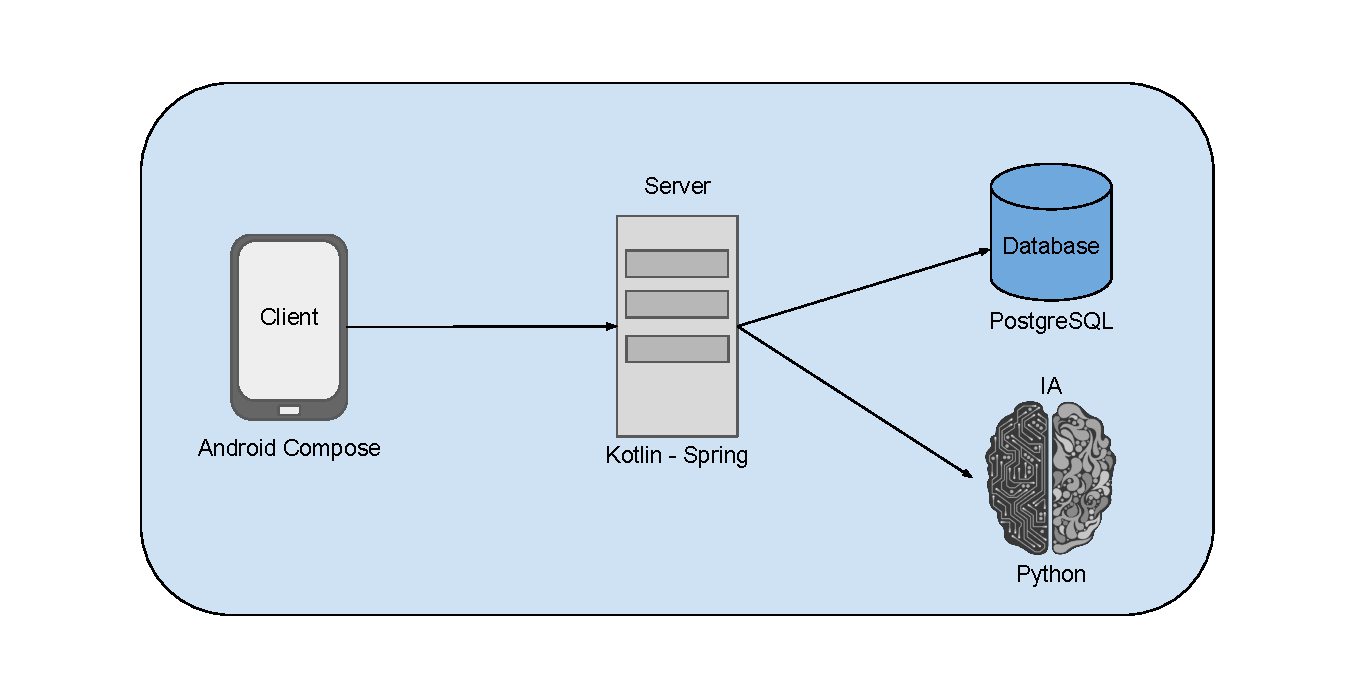
\includegraphics[width=0.9\textwidth]{./Chapter3/Figures/Project Structure}
	\caption{Project Architecture}
	\label{fig:PStruct}
\end{figure}


\subsection{Signing In}
To be able to use any of the provided functionalities its necessary for the user to sign in the service. Signing In can be either a login operation or a register operation. Its required for the user to have a valid phone number in order to perform either one of the operations.
Once registered the user will have access to all of the service functionalities.

\subsection{Connecting to Friends}
Connecting to friends in the service is simple, no need to find for a specific username simply give access to the user's phone numbers and the service will provide you with the contacts registered in it.   

\subsection{Obtaining Templates}
A template represents a potential postcard background. Every application developed to use this Web API needs to have consistency, that is, it needs to keep the templates up-to-date with the ones stored in the server.


\subsection{Creating Chat Groups}
Once registered the user can now create chats groups. These chat groups are made up of all the people the users is meant to send a postcard and/or receive from.
When sending a postcard to someone a chat group is required.  

\subsection{Sending Messages (Postcards)}
A message is referenced in this report and throughout the application development as a holder for the postcard. A message contains more information besides the postcard itself (we will delve deeper about messages in the report \ref{subsec:Message}).
Sending a postcard involves choosing a postcard template (the background of the postcard) and  writing to it. 
Internally the postcard is represented by two layers, the template and the written content, both of which are SVG's \textit{\cite{SVG}}, allowing for high quality postcards. 

\subsection{Handwriting Text Recognition}
For each message a request can be made to extract the drawn text contained in it to computer digits. To perform such operation only the drawn content is needed.

\bigskip

\paragraph{Application Flow}

The application flow can be seen in Figure~\ref{fig:AppFlow}.

\begin{figure}[!ht]
	\centering
	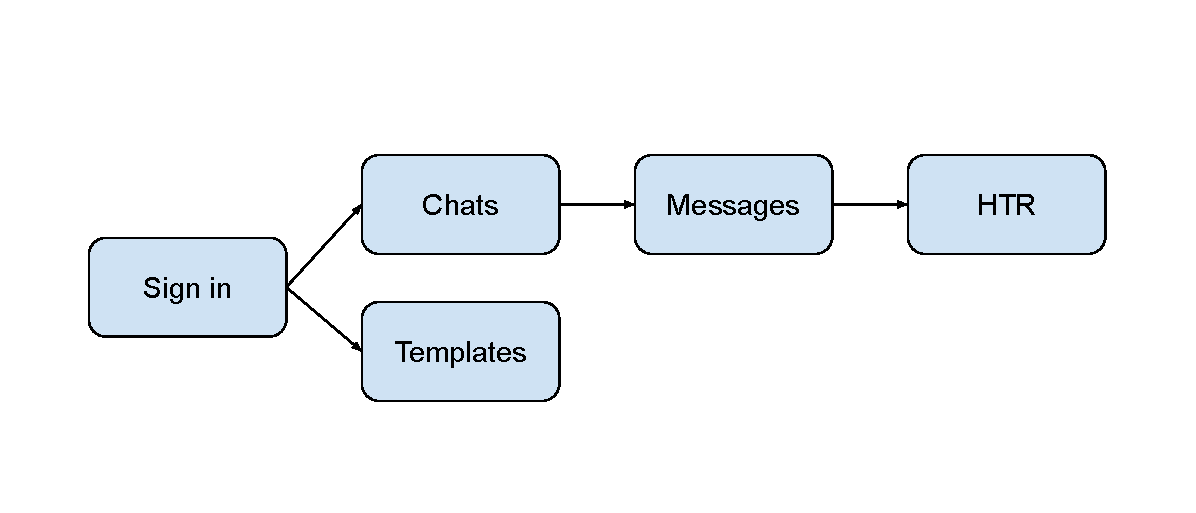
\includegraphics[width=0.75\textwidth]{./Chapter3/Figures/Application Flow}
	\caption{Application Flow}
	\label{fig:AppFlow}
\end{figure}


%////////////////////////////////////////////////////////////////////////
%   Chapter 4
%
%////////////////////////////////////////////////////////////////////////
\chapter{Development support} 
\label{ch:Chapter4}
\vfill \minitoc \newpage

\section{Azure DevOps Services}

To ease development the group decided to use \textit{\cite{azuredevops}}. This platform provides development collaboration tools along with mechanisms that allow for a better work environment that follow DevOps practices.

Figure~\ref{fig:DevopsTasks1} illustrates DevOps Work Items (Azure Boards).

From the many tools provided by the service, the following are the ones used in this project:
\begin{itemize}
	\item Azure Boards
	\item Azure Repos
	\item Azure Pipelines
	\item Azure Artifacts
\end{itemize}


\begin{figure}[!ht]
	\centering
	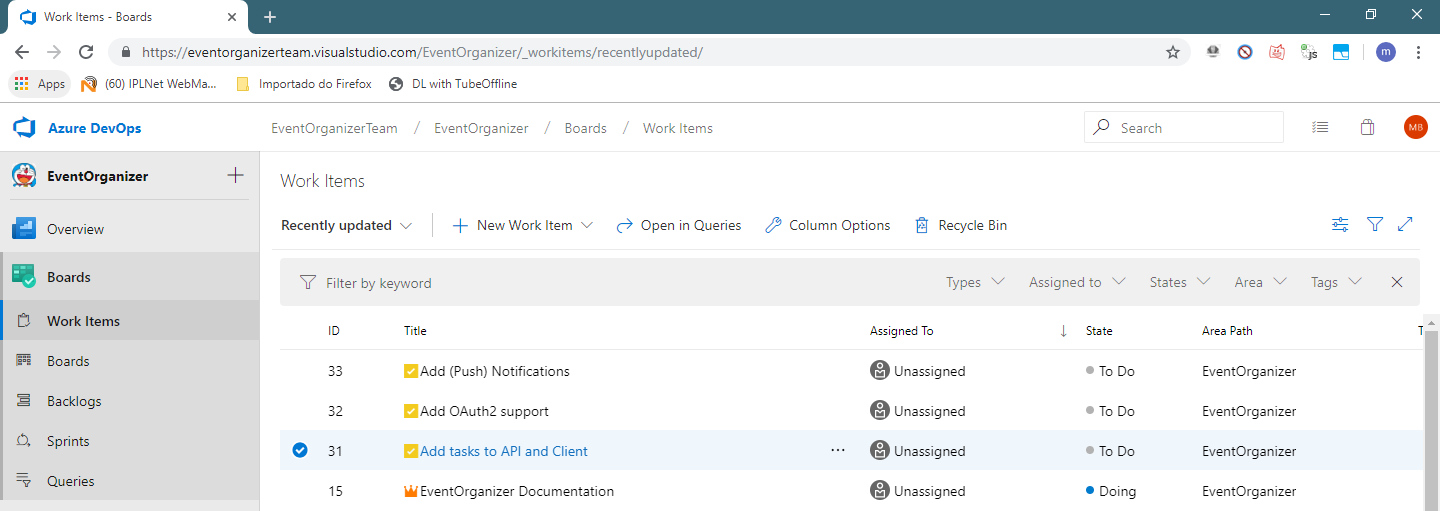
\includegraphics[width=0.75\textwidth]{./Chapter4/Figures/DevopsTasks1.png}
	\caption{DevOps Boards Work Items}
	\label{fig:DevopsTasks1}
\end{figure}

\subsection{Azure Repos}
Azure Repos is a set of version control tools, allowing for multiple repositories, each one having its own version control system. For this project four repositories where created:

\begin{itemize}
	\item EventOrganizer.WebApi – Where the source code for the EventAPI and its HTTP Client is maintained.
	\item EventOrganizer.Client – Where the Xamarin client application source code is maintained.
	\item EventOrganizer.Database – Repository containing the scripts and backups for database management.
	\item EventOrganizer.Documentation – Dedicated to gather project documentation used in development.
	\item EventOrganizer.MusicApi – Contains the source code for the Music Web Api and its HTTP Client.
\end{itemize}

Figure~\ref{fig:BranchingStrategy} illustrates the feature branching strategy used.

Wanting to keep the development repositories, EventOrganizer.WebApi, EventOrganizer.MusicApi and EventOrganizer.Client organized and easy to maintain, the group decided to use the following branching strategy:

\begin{figure}[!ht]
	\centering
	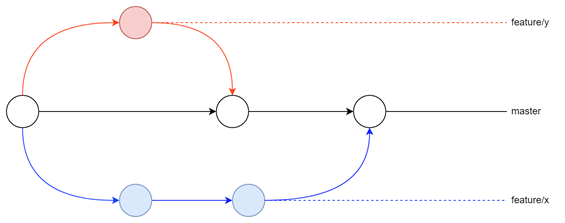
\includegraphics[width=0.75\textwidth]{./Chapter4/Figures/BranchingStrategy.png}
	\caption{Feature Branching Strategy}
	\label{fig:BranchingStrategy}
\end{figure}

This branching strategy consists of creating a feature branch for each new functionality that needs to be implemented. This, combined with frequent pull requests, helped the team maintaining the source code, making sure the master branch always had a stable version and making bugs less frequent and smaller problems to resolve.

\subsection{Azure Pipelines}
Azure Pipelines is a service that can be used to build, test and deploy projects by having remote machines run a preconfigured pipeline.

For this project the group configured three pipelines:

\begin{itemize}
	\item Event Web API Pipeline – Builds the EventAPI project and deploys the Web API to Azure App Services.
	\item Generate Client Nugets – Builds and packages the EventAPI HTTP client libraries into nuget packages that contain versioning.
	\item Event Web API Pipeline – Builds the EventAPI project and deploys the Web API to Azure App Services.
	
\end{itemize}

The first two pipelines are queued for execution every time there is a new stable version, meaning every time there is a push to the master branch.

\subsection{Azure Artifacts}
Azure Artifacts gave the team the possibility of having a private nuget feed where the nuget packages generated in the Azure Pipelines are automatically pushed. This service comes with a page in Azure DevOps, where the nugets can also be viewed and managed.

\subsection{Pull Requests}

To keep code versioning efficient and organized, the decision to block direct pushes to the master branch was made.

When a feature is complete, instead of merging the feature branch to the master branch, a pull request must be open and reviewed before being completed, which results in an automatic merge to the master branch.

In addition to the mandatory review of the code, pull requests must also pass a build pipeline configured for each repository. This was done by first creating a new Azure Pipeline for each repository that builds and tests the respective solutions and secondly adding a build policy for the master branch, which specifies that the previously created pipeline should run to completion successfully.

The page for a pull request where the required policies include the previously mentioned code review, build and test run can be seen in the screen capture below.

\begin{figure}[!ht]
	\centering
	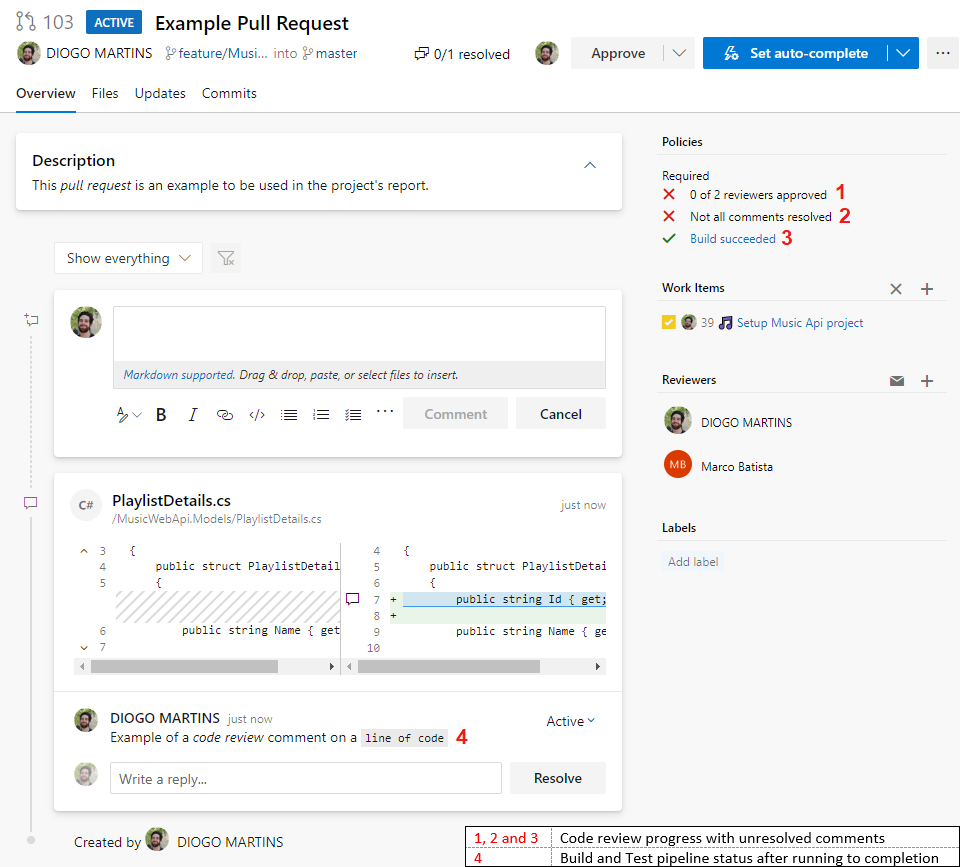
\includegraphics[width=0.75\textwidth]{./Chapter4/Figures/PullRequestExample.png}
	\caption{An example of a pull request in the development repositories}
	\label{fig:PullRequestExample}
\end{figure}

\newpage

\section{Other tools}
The group is also using Microsoft Visual Studio as it's main programming IDE as it's really flexible and it's integration with Nuget, Xamarin and UWP is seamless to the group and offers (almost) no problems and Jetbrains DataGrip as the main database IDE (although sometimes the group also uses pgAdmin for more low level operations on the PostgreSQL database).



\section{Architecture}

Figure~\ref{fig:SystemArchitecture} illustrates the system architecture.

\begin{figure}[!ht]
	\centering
	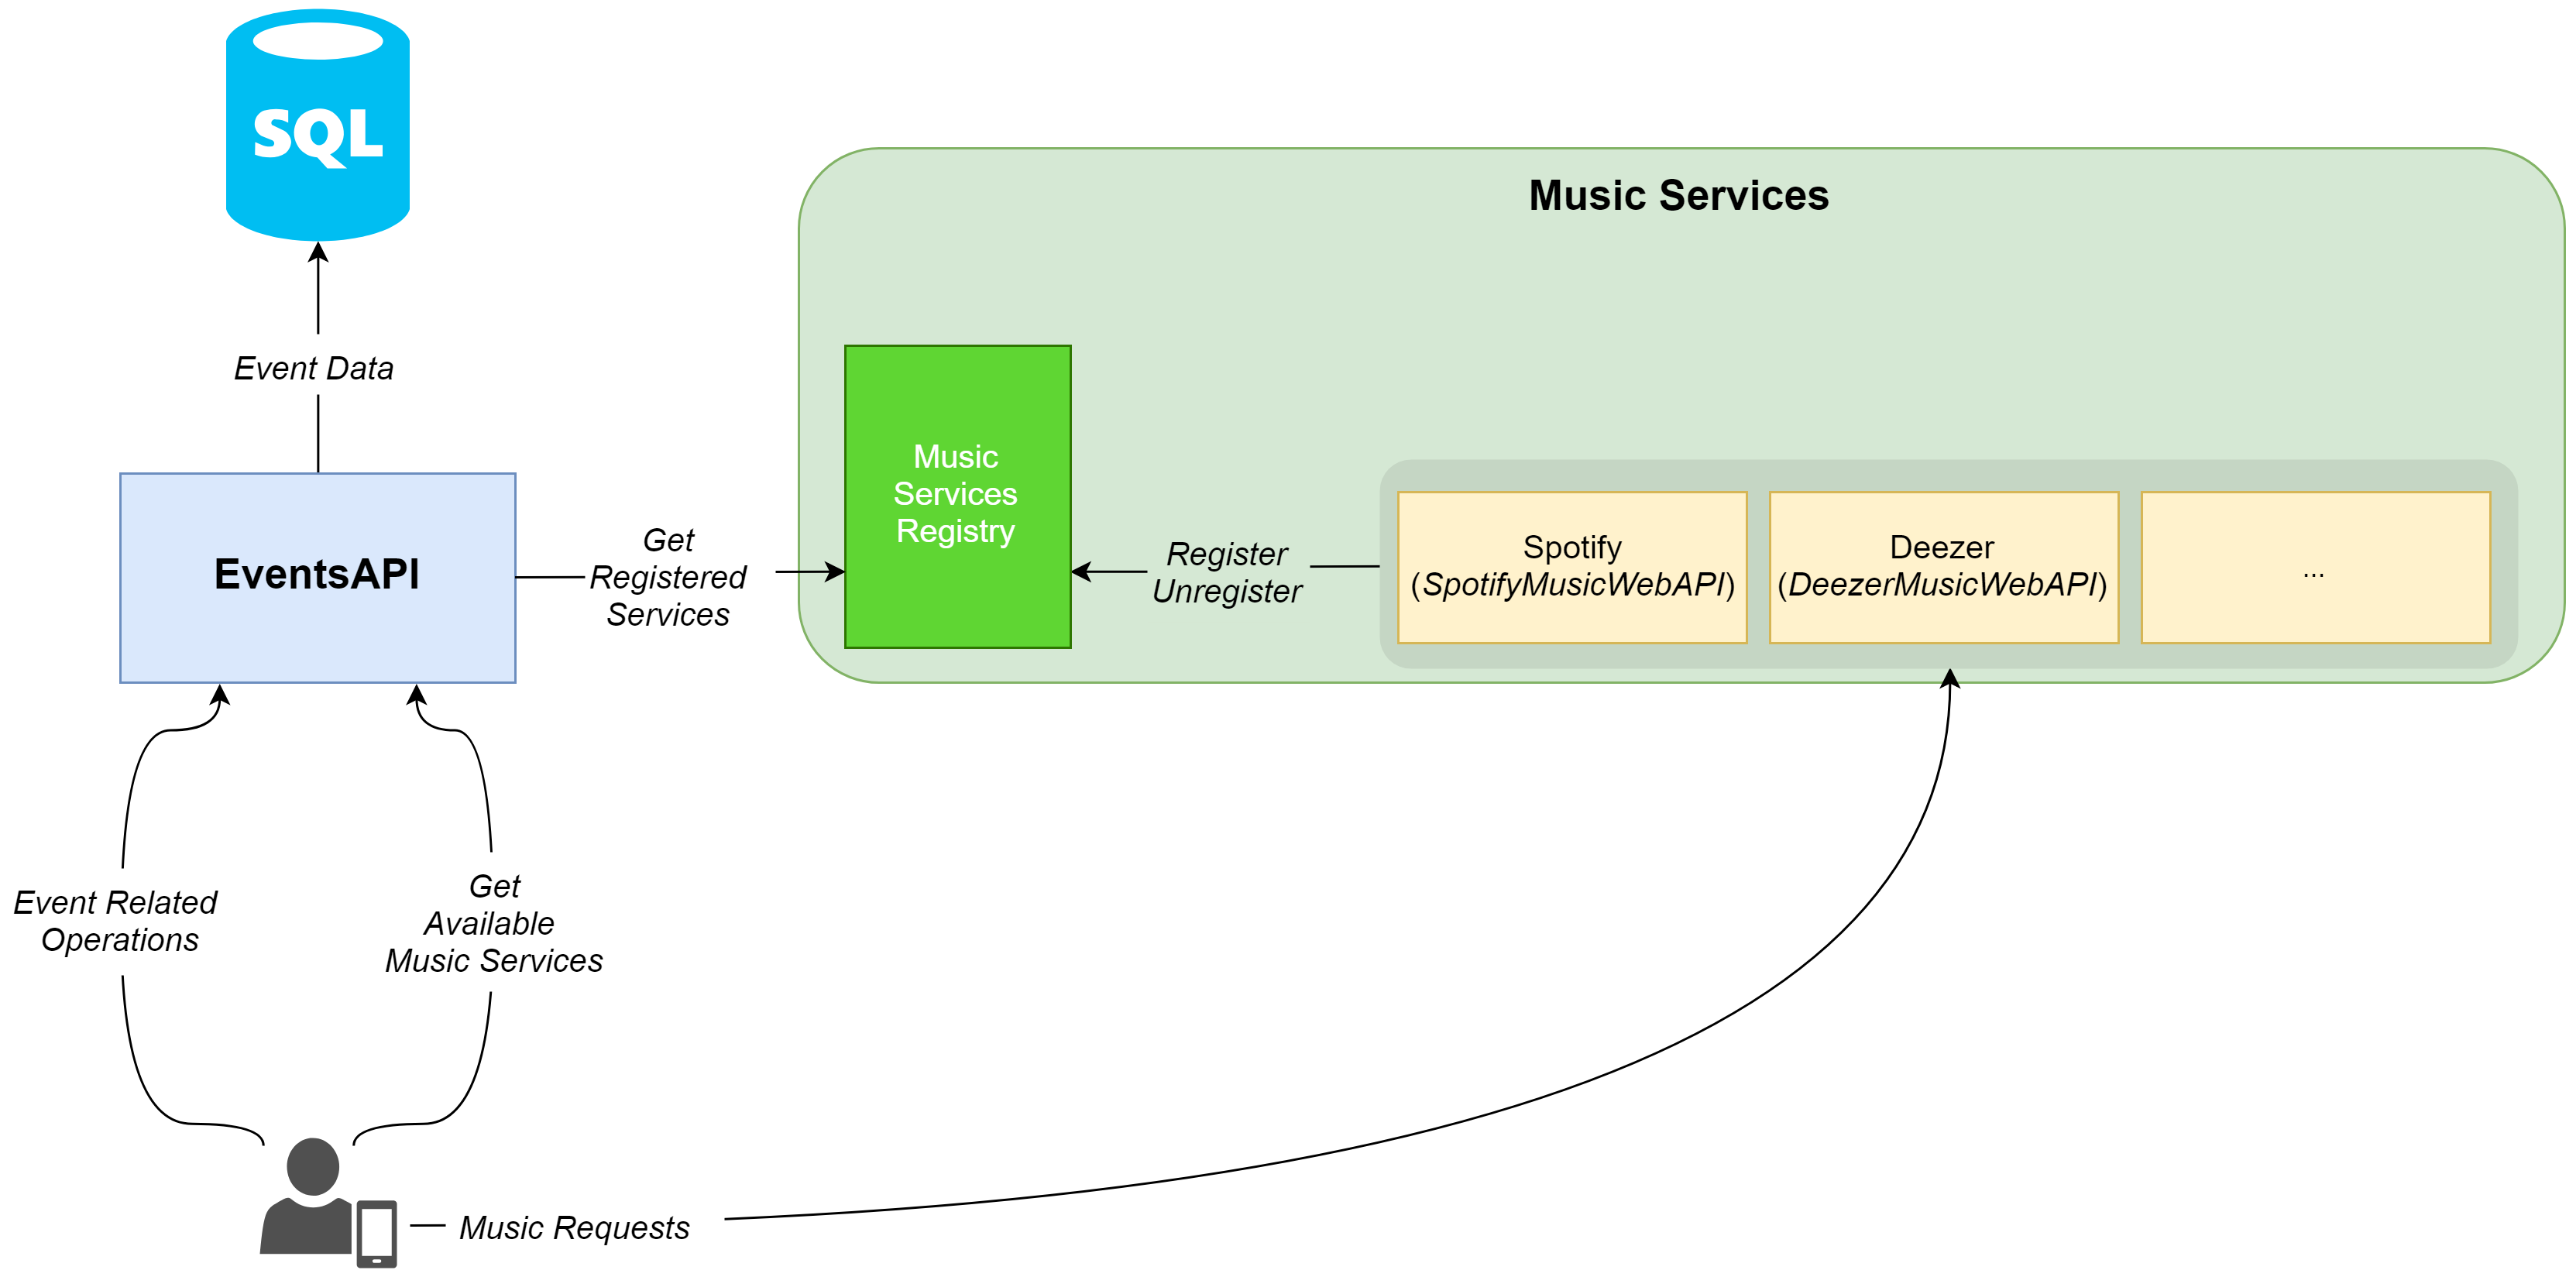
\includegraphics[width=0.75\textwidth]{./Chapter4/Figures/Architecture.png}
	\caption{System architecture.}
	\label{fig:SystemArchitecture}
\end{figure}

\subsection{Client}

The client component of this project is implemented as a mobile application, using the \textit{Android} and \textit{Windows} platform.

\subsection{Server}

The server component is implemented as a REST API, using .NET Core MVC.
\begin{itemize}	
	\item Event API - Supports the event creation and all of its operations (adding, editing and removing guests, expenses, tasks, among others);
	
	\item Music API - Supports the \textit{playlist} creation;
	
	\item Payments API (optional) - Supports the payment of the event's expenses.
	
\end{itemize}

The database operations are supported by the PostgreSQL database engine.

\subsubsection{Observations}

The motivation behind choosing this server-client architecture is the possibility of eventually creating other clients, without having to change the servers that support it.

The reason why the Payments and Media API aren't unified into the Event API is for the sake of having the benefit of the client only communicating with these APIs, yet having the possibility of comunicating with a wide range of services without having to implement them specifically.

The motivation behind the usage of SQL instead of NoSQL database types is because the entities used in this application are of relational types. Also, the atomicty and transactional behaviour that SQL databases support is of importance for consistency across event information.




%/////////////////////////////////////////////////////////////
%   Chapter 5
%   Web Client implementation
%
%/////////////////////////////////////////////////////////////

\chapter{HTR Model} 
\label{ch:Chapter5}
\vfill \minitoc \newpage

\section{Introduction}
Handwriting recognition \gls{htr} is a technology that converts handwritten text into digital format. Its purpose is to enable the efficient processing, storage, and manipulation of handwritten content through automated recognition algorithms.

\subsection{Offline HTR}
Offline handwriting recognition refers to the technology and process of converting static images or scans of handwritten text into digital text or characters. Unlike online handwriting recognition, which interprets handwriting in real time as it is being written, Offline \gls{htr} analyzes pre-existing images or documents that have been captured or scanned.

The goal of Offline \gls{htr} is to accurately recognize and convert the handwritten text in images into editable and searchable digital format. This technology finds applications in digitizing historical documents, handwritten notes, forms, and any other handwritten content that needs to be converted into machine-readable text.

The process of Offline \gls{htr} typically involves several steps:
\begin{itemize}
    \item Detection: In the detection phase, the handwritten text regions within the scanned or captured images are identified. This can be achieved through techniques such as text detection algorithms, connected component analysis, or contour-based methods. The goal is to localize and extract the regions containing the handwritten content for further processing.

    \item Image preprocessing: The scanned or captured images are enhanced, filtered, and prepared to optimize the quality of the handwriting for recognition. This may involve noise reduction, binarization, deskewing, and other techniques.
    
    \item Recognition: Machine learning algorithms, such as neural networks or Hidden Markov Models (HMM), are trained using labeled samples of handwritten characters or words. These models are then used to recognize and classify the extracted features into corresponding textual representations.

    \item Post-processing: The recognized text is further refined and processed to improve accuracy, correct errors, handle ambiguities, and align with language-specific rules and dictionaries.

\end{itemize}


\subsection{Online HTR}
Online handwriting recognition refers to the technology and process of converting handwritten input into digital text or characters in real time. It involves capturing and interpreting the movements and patterns made by a user while writing using a stylus or a digital pen on a touch-enabled device, such as a tablet or a smartphone.

Unlike offline handwriting recognition, which analyzes static images of handwritten text, online handwriting recognition takes advantage of the temporal information obtained during the writing process. This allows for real-time interpretation and immediate feedback as the user writes, making it suitable for applications where instant recognition is required, such as note-taking, electronic signature verification, form filling, and interactive whiteboards.

Online handwriting \textit{\cite{OnlineHTR}} recognition systems typically use various techniques, including pattern recognition algorithms, machine learning, and neural networks, to analyze the dynamic information provided by the user's pen strokes. These algorithms analyze factors such as stroke speed, direction, pressure, and sequence to identify and interpret the handwritten characters or gestures. The recognized text can then be further processed, stored, or used in various applications and systems that require digital text input.


\section{Implementation}
In this section we will talk about the decisions made and explain the implementation of each component.
\subsection{Why Offline HTR}
In a project like this, it initially seems like a no-brainer to implement Online \gls{htr} instead of Offline \gls{htr}. However, the lack of complex yet comprehensive documentation for beginners pose a significant roadblock. Without readily available resources and clear guidance, the implementation process becomes more complex and time-consuming. This led to frustration and delays as the we struggled to navigate the complexities of Online \gls{htr} without proper guidance.

Furthermore, the absence of open-source implementations of Online \gls{htr} hinders collaboration and knowledge sharing within the community. Open-source projects often serve as valuable starting points, providing code samples, libraries, and frameworks that accelerate the development process. Without such resources, we must start from scratch or rely on proprietary solutions, limiting the ability to customize and adapt the \gls{htr} system to the specific project requirements. The potential benefits of enhanced accuracy,  real time text recognition, and dynamic input support opportunities may be overshadowed by the steep learning curve and lack of accessible resources for offline \gls{htr} implementation.

As a result, the decision to implement Offline \gls{htr} becomes less straightforward yet possible thanks to widely available open-source implementations and good guidance examples such as the one followed to implement our model \textit{\cite{HTR}}.


\subsection{Pipeline}
The \gls{htr} system follows a pipeline-based approach to process images and extract text. The pipeline consists of two main stages: text detection and text recognition.
The Figure~\ref{fig:HTRS} represents a overview of the implemented \gls{htr} system. For our needs it takes a PNG containing the postcard drawn content and returns the text as a String. 

\begin{figure}[!ht]
	\centering
	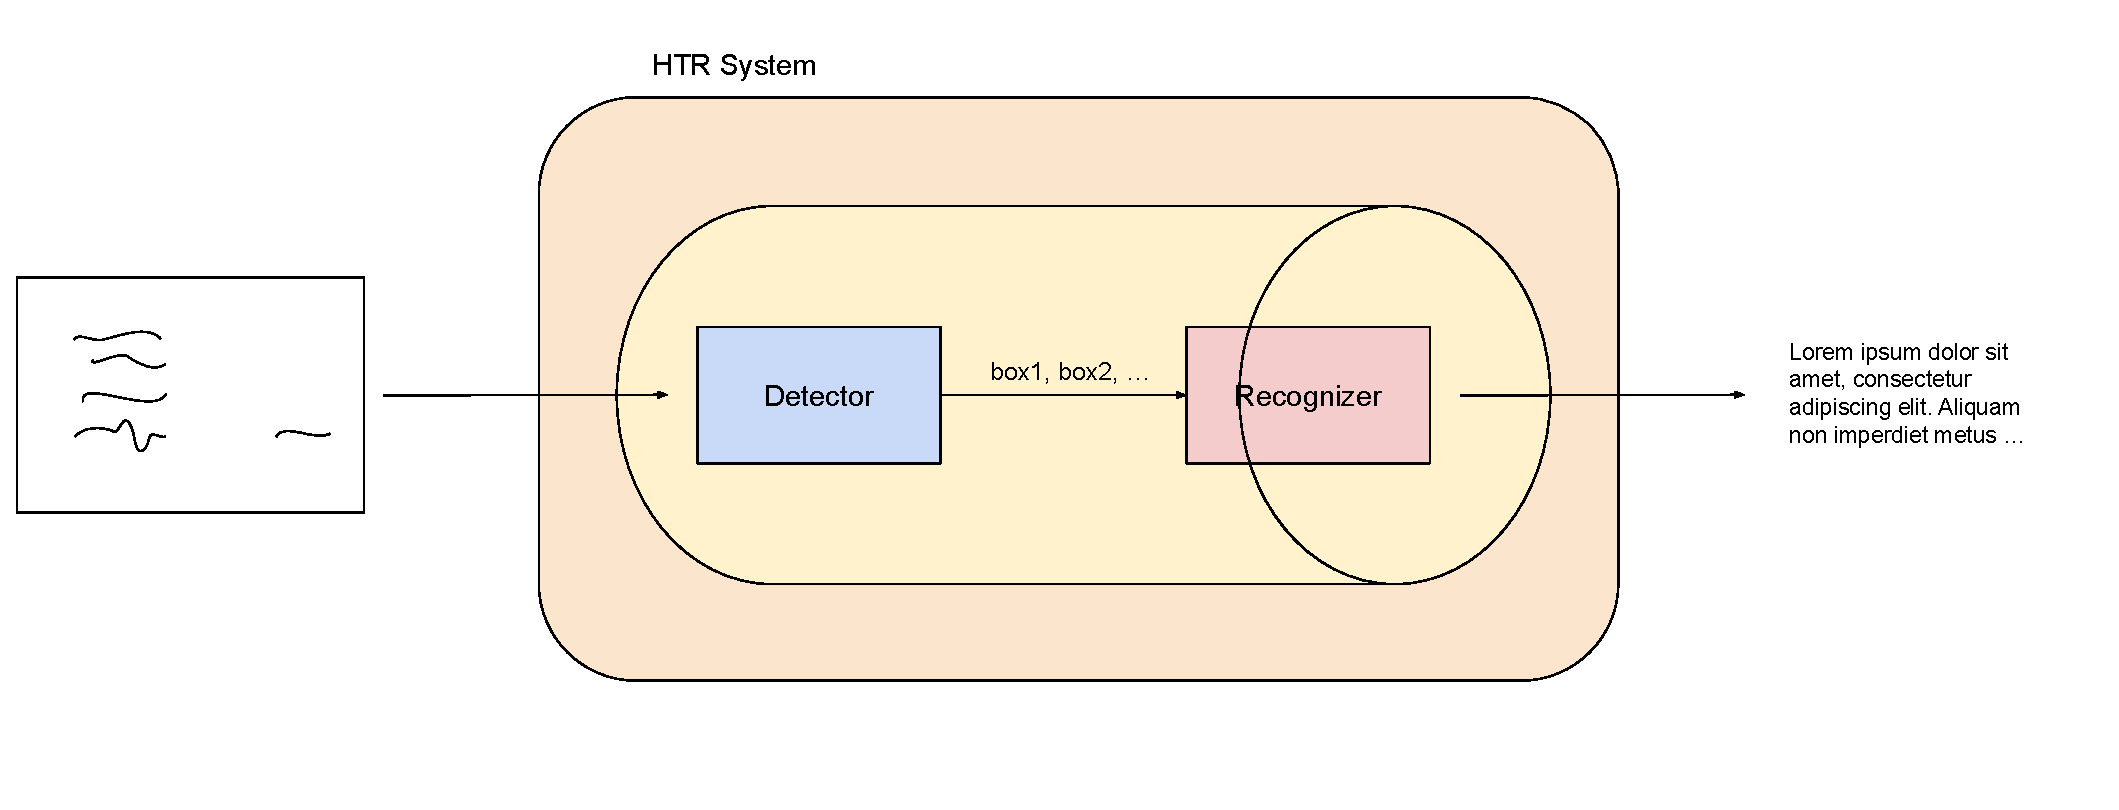
\includegraphics[trim={ 0.2cm 1cm 0cm 0cm },width=1\textwidth]{./Chapter5/Figures/HTR System}
	\caption{HTR System}
	\label{fig:HTRS}
\end{figure}

\textbf{Both components use the Tensorflow framework and are written in python.}

\subsection{Detector}
The detection is made possible by using CRAFT-Text \textit{\cite{CRAFT-Text}} detection implementation from \textit{\cite{Keras-ocr}}. The particular detector was trained for machine-generated characters based on fonts but still manages to give good results for handwritten text, big part of it's good results is the absence of visual clutter in the background as we only provide the drawn content to the model. 


The Figure~\ref{fig:Detector} illustrates how the detector works, keeping in mind that the figure is simplified for explanatory purposes and the detector detects words and not lines.

\begin{figure}[!ht]
	\centering
	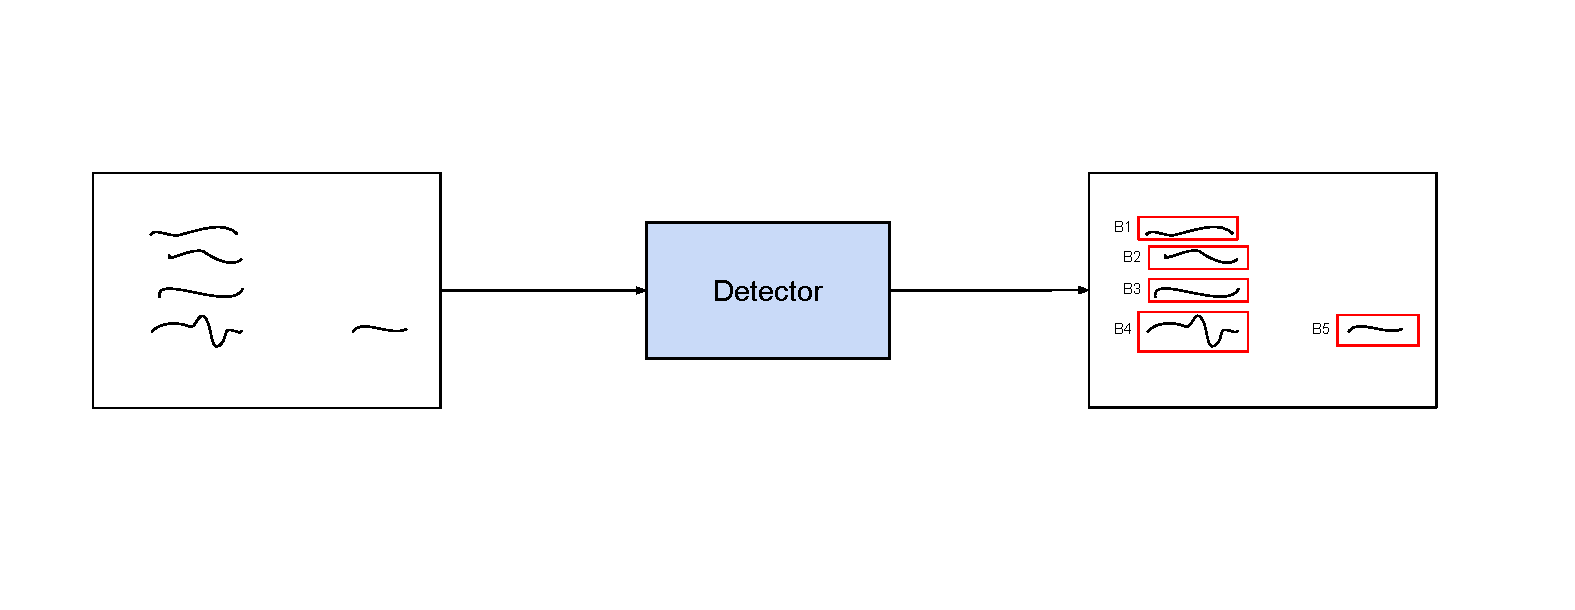
\includegraphics[trim={2cm 3cm 0 1cm}, width=1.1\textwidth]{./Chapter5/Figures/Detector}
	\caption{Detection Flow}
	\label{fig:Detector}
\end{figure}

The returned value from the detector model is a list containing four points (x and y) defining a box that represents where the word is relative to the image.


\subsection{Recognizer}
The text recognition stage takes the boxes from the detector and processes them to extract the actual text content creating a temporary file for each box. It applies character segmentation, feature extraction, and sequence modeling techniques to recognize and convert the text regions into machine-readable format. A layer by layer summary based on online documentation:
\begin{itemize}
    \item Input Layer: The model takes an input image with dimensions (128, 32, 1), representing a grayscale image. It also takes input labels, which are sequences of characters.
    \item Convolutional Layers: The model starts with two convolutional blocks. Each block consists of a 2D convolutional layer followed by a max-pooling layer. The convolutional layers learn local image features and the max-pooling layers downsample the feature maps.
    \item Reshaping and Dense Layer: After the convolutional layers, the feature maps are reshaped to a new shape that is compatible with the recurrent part of the model. This reshaping operation prepares the data for input to the recurrent layers. The reshaped features pass through a fully connected dense layer with 64 units and ReLU activation.
    \item Dropout Regularization: A dropout layer is applied to reduce overfitting by randomly setting a fraction of the input units to 0 during training.
    \item Recurrent Layers: Two bidirectional LSTM layers are stacked on top of each other. Bidirectional LSTMs process the input sequence in both forward and backward directions, allowing the model to capture dependencies in both directions. The LSTM layers have dropout applied to them to prevent overfitting.
    \item Output Layer: A dense layer with a softmax activation is used as the output layer. The number of units in this layer corresponds to the vocabulary size (number of characters) plus two special tokens introduced by the CTC loss. The softmax activation produces a probability distribution over the characters.
    \item CTC Loss Layer: The output of the softmax layer is passed to the Connectionist Temporal Classification (CTC) layer. The CTC layer calculates the CTC loss, which measures the difference between the predicted sequence and the ground truth labels. It takes both the labels and the output of the softmax layer as inputs.
    \item Model Compilation: The model is compiled with the Adam optimizer. The specific learning rate and other optimizer parameters can be further customized if needed.
    \item Model Output: The output of the model is the output of the CTC layer, representing the CTC loss. 

\end{itemize}


\begin{figure}[!ht]
	\centering
	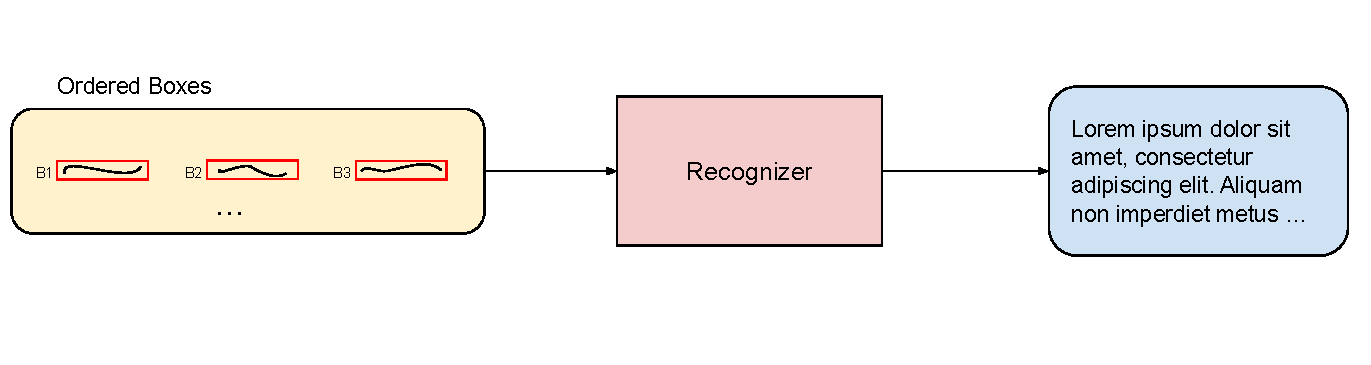
\includegraphics[trim={0cm 0cm 0 0cm}, width=1\textwidth]{./Chapter5/Figures/Recognizer}
	\caption{Recognizer Flow}
	\label{fig:Recognizer}
\end{figure}




\subsubsection{Image Preprocessing}
Image preprocessing is a critical step in offline \gls{htr} systems as it aims to enhance the quality of scanned or captured handwritten images before they are fed into the recognition model. The objective is to optimize the images for accurate recognition by applying various transformations and adjustments.

In the context of our project, the provided code snippet offers a foundational approach to image preprocessing.

Reading and Decoding Image:

The first step involves reading the image file using tf.io.read\_file and decoding it using tf.image.decode\_png.
By decoding the image as grayscale (decode\_png(image, 1)), we ensure that only the necessary information is retained.
Distortion-Free Resizing:

To achieve consistent input sizes, the distortion\_free\_resize function is employed for resizing the image to the desired dimensions (img\_size).
During resizing, the preserve\_aspect\_ratio=True parameter ensures that the original aspect ratio of the image is maintained.
This function intelligently pads the image symmetrically to ensure uniformity and prevent distortion.
Normalization:

After resizing, the image is cast to tf.float32 and normalized to a range between 0 and 1 by dividing each pixel value by 255.0.
Normalization facilitates improved convergence during training and enhances the overall performance of the recognition model.
By utilizing the preprocess\_image function, we establish a solid foundation for handling image preprocessing in our offline \gls{htr} system. This function accepts an image path as input and performs resizing, padding, and normalization operations to prepare the image for subsequent processing.


\subsubsection{Training}
The recognizer was trained using the \textit{\cite{IAM}} words dataset, which is a widely used benchmark dataset for \gls{htr} research. The IAM dataset is a comprehensive collection of handwritten English text samples contributed by different writers. It consists of 86810 training samples, 4823 validation samples and 
4823 test samples.

To get good results the recognizer was trained for roughly 60 iterations in Google's Colab Notebook servers.

\paragraph{Tweaks}
After each training iteration, the Tensorflow training process incorporates additional code through callbacks to enhance its functionality. In this particular scenario, two tweaks have been added to optimize the training process:
\begin{itemize}
    \item Early Stopping Callback:
    An early stopping callback is implemented to monitor the model's performance during training and determine if it is not improving.
    The patience parameter is set to 3, indicating that if the model does not show improvement for 3 consecutive iterations, the training process will stop early.
    By setting restore\_best\_weights to True, the callback ensures that the best weights achieved during training are restored before stopping, allowing for optimal model performance.
    The verbose parameter is set to 1, enabling the callback to display informative messages about its operations. 
    \item Checkpoint Callback:
    A checkpoint callback is added to periodically save the model's weights during training.
    The filepath parameter specifies the path where the weights will be saved.
    By setting save\_weights\_only to True, only the weights of the model will be saved, reducing storage requirements.
    The verbose parameter is set to 1, enabling the callback to display informative messages about the saving process.
\end{itemize}

These tweaks improve the training process by introducing early stopping criteria based on the model's performance and by providing checkpoints to save the model's weights at different stages.


\subsubsection{Postprocessing}
To be able to decode the output produced by the Output Layer (dense 2) a function called  \textit{decode\_batch\_predictions} is implemented in the guide \textit{\cite{HTR}}.

The function takes the model predictions pred as input. These predictions are usually in the form of probability distributions over the characters in the vocabulary for each time step.

The variable input\_len is created to specify the length of the input sequences for each prediction in the batch. It is set to be the same for all predictions and is equal to the number of time steps in the predictions.

The function utilizes the CTC (Connectionist Temporal Classification) decoding method to convert the predictions into sequences of characters. It applies the ctc\_decode function from Keras backend, passing the predictions, input length, and using greedy search (other methods like beam search can be used for more complex tasks). The ctc\_decode function returns the decoded sequences.

The results variable stores the decoded sequences. It selects the first element [0][0] from the ctc\_decode output, which represents the decoded labels for the batch. It also truncates the sequences to a maximum length max\_len if necessary.

The function iterates over each decoded sequence in results. For each sequence, it applies several operations to convert the numerical labels to actual text.

First, it uses tf.where to find the positions where the labels are not equal to -1 (a special token often used in CTC decoding to represent blank or no label).

It then uses tf.gather to gather the non-equal elements from the labels.

The gathered labels are passed through num\_to\_char function, which maps the numerical labels to their corresponding characters.

Next, tf.strings.reduce\_join is applied to concatenate the characters into a single string representation.

Finally, numpy().decode("utf-8") is used to convert the string from a TensorFlow tensor to a regular Python string, and the resulting string is appended to the output\_text list.

After iterating over all the sequences in results, the function returns the output\_text list, which contains the decoded texts for each prediction in the batch.

In summary, the decode\_batch\_predictions function takes the model predictions, performs CTC decoding to convert the predictions into sequences of characters, and applies additional post-processing steps to obtain the final text representations for the predictions.


\subsection{Natural Text Ordering}
One of the challenges in \gls{htr} is maintaining the natural ordering of text when dealing with multi-line or multi-column documents. To address this challenge, we came up with a algorithm that uses the average box size to calculate a margin of error for each point in a line.
In our implementation there is always two fixed boxes Figure~\ref{fig:PFBoxes}

\begin{figure}[!ht]
	\centering
	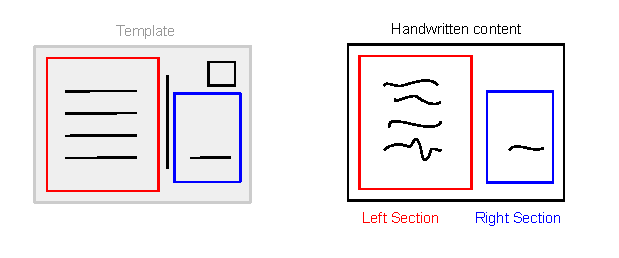
\includegraphics[trim={0cm 0cm 0 0cm}, width=1\textwidth]{./Chapter5/Figures/Main Sections Postcard}
	\caption{Postcard Main Sections}
	\label{fig:PFBoxes}
\end{figure}

\newpage

The ordering algorithm works like this:

We start by calculating the height of every box, using vector calculation. We do this for every box and divide by the number of boxes obtaining the average box height.

\begin{figure}[!ht]
	\centering
	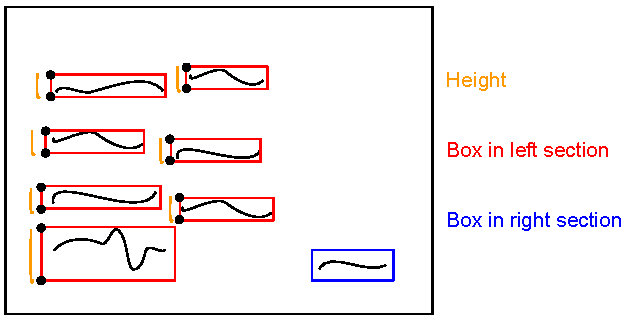
\includegraphics[trim={0cm -0.5cm 0 -0.5cm}, width=0.7\textwidth]{./Chapter5/Figures/Height Box}
	\caption{Average height calculation for left section}
	\label{fig:AVGH}
\end{figure}


Now all we have to do is pick the same located point in every box (top left or right left, etc...) and test the y value +- the calculated average box/2. If the y value is inside the range y-average height/2 to y+average height/2 then compare the x values else compare the y values. A lower x value means it comes earlier in the natural ordering. A higher y value than the current one means it comes later in the natural ordering. 

\section{Limitations}
IAM dataset vocabulary is primarily focused on the English language. It includes a wide range of alphanumeric characters, including uppercase and lowercase letters (A-Z, a-z), digits (0-9), and common punctuation marks. However, it does not cover the entire spectrum of possible characters that can exist in different languages or writing systems.

This vocabulary limitation means that the IAM dataset may not be suitable for recognizing text in languages other than English or for dealing with specialized symbols or characters that are outside the dataset's predefined set. For example, if the dataset does not include characters specific to a particular language or domain, the \gls{htr} model trained on IAM may struggle to accurately recognize and transcribe such characters.

While having made all the possible optimizations for using the detector, if the user draws text right next to each other there's a good change it will detect it all as a whole word.

\section{Results}
Results tend to vary a lot depending on the input image. 

Thicker line strokes, angled letters and image quality are some of the factors that directly influence the final output.

Higher quality images (more pixels) and thinner stroke lines tend to get better results.

These are the obtained results:
\begin{itemize}
	\item Figure~\ref{fig:T1} - Thiss is a tost image with arial font Hollo MHTPR model
	\item Figure~\ref{fig:T2} - Heito Worild Thiss is a HT. modet DoRs It works Antonio Canvatho
	\item Figure~\ref{fig:T3} - This is a tost Mello world Can you read thist 
	\item Figure~\ref{fig:T4} - this is a Tasst
\end{itemize} 

\begin{figure}[!ht]
	\centering
	\fbox{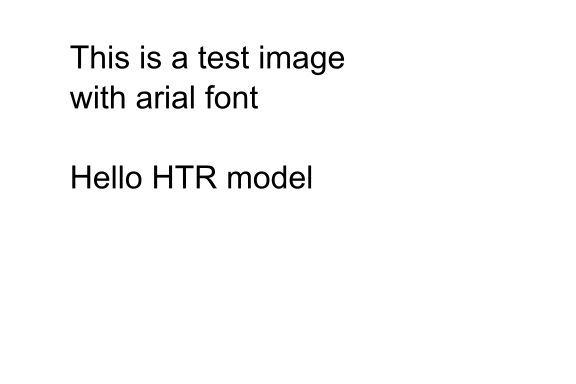
\includegraphics[trim={0cm -0.5cm 0 -0.5cm}, width=0.7\textwidth]{./Chapter5/Figures/test1}}
	\caption{Test figure 1}
	\label{fig:T1}
\end{figure}

\begin{figure}[!ht]
	\centering
	\fbox{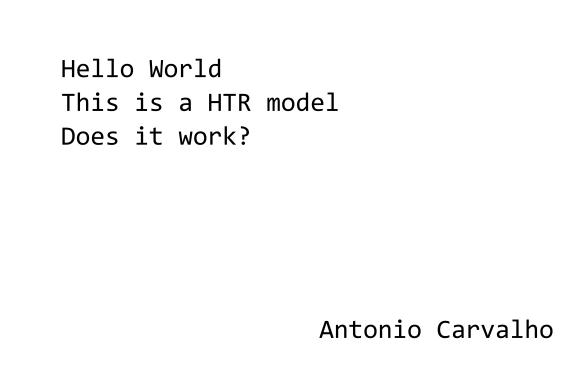
\includegraphics[trim={0cm -0.5cm 0 -0.5cm}, width=0.7\textwidth]{./Chapter5/Figures/test2}}
	\caption{Test figure 2}
	\label{fig:T2}
\end{figure}


\begin{figure}[!ht]
	\centering
	\fbox{
\includegraphics[trim={0cm -0.5cm 0 -0.5cm}, width=0.7\textwidth]{./Chapter5/Figures/test3}}
	\caption{Test figure 3}
	\label{fig:T3}
\end{figure}


\begin{figure}[!ht]
	\centering
	\fbox{
\includegraphics[trim={0cm -0.5cm 0 -0.5cm}, width=0.7\textwidth]{./Chapter5/Figures/test4}}
	\caption{Test figure 4}
	\label{fig:T4}
\end{figure}






%/////////////////////////////////////////////////////////////
%   Chapter 6
%   Results
%   
%
%/////////////////////////////////////////////////////////////
\chapter{Client} 
\label{ch:Chapter6}
\vfill \minitoc \newpage

The client was implemented in Android and uses Android's Jetpack Compose UI toolkit.

\begin{figure}[!ht]
	\centering
	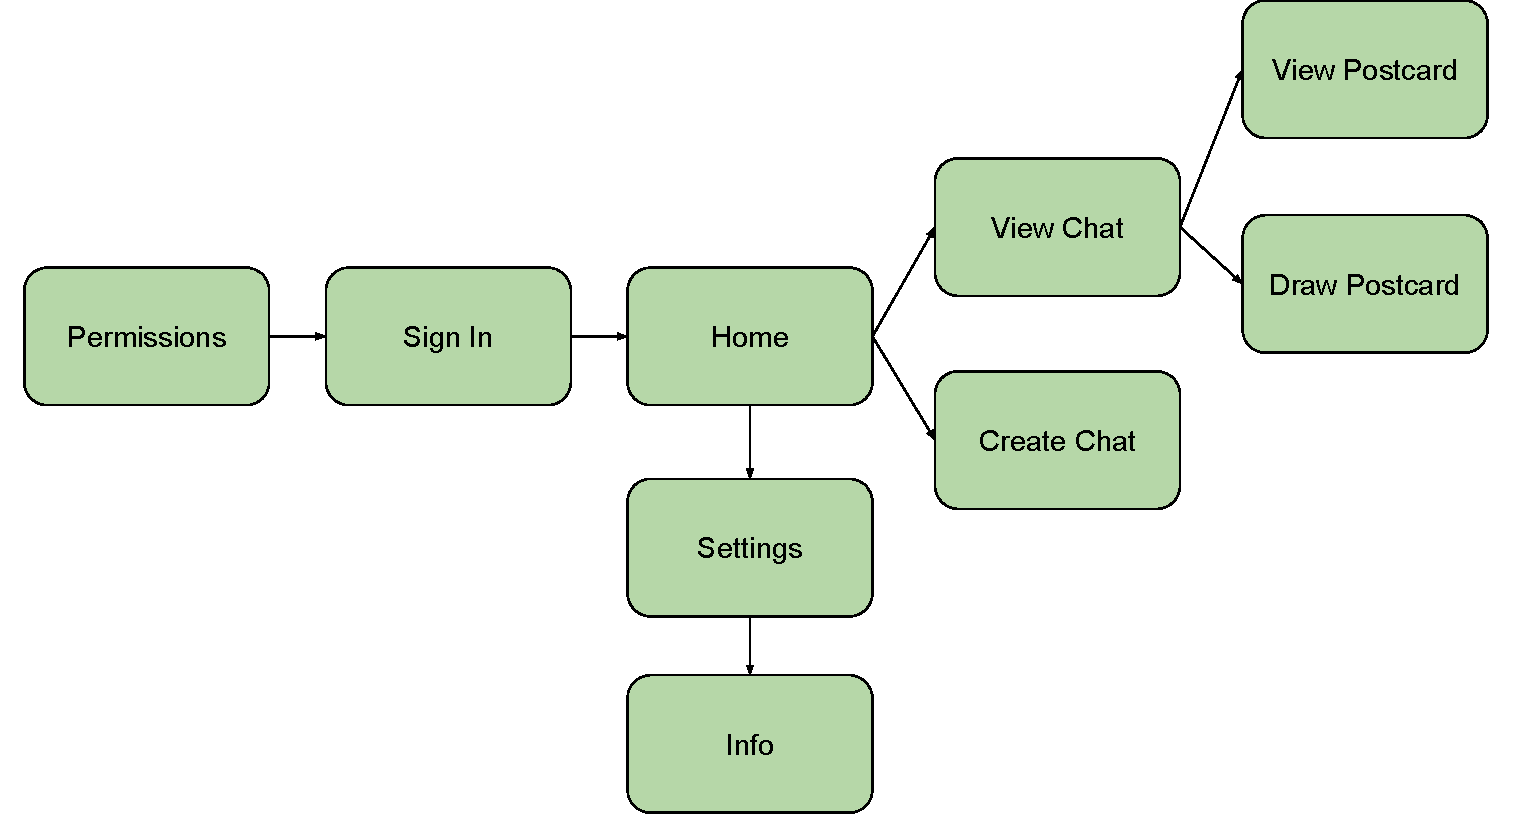
\includegraphics[trim={0cm 0cm 0 0cm}, width=1\textwidth]{./Chapter6/Figures/Android NavGraph}
	\caption{Android Activity Navigation Graphic}
	\label{fig:NavgGraph}
\end{figure}


\section{Android System and Compose Framework Overview}
Before showing the client implementation its best to give some context and basic knowledge about the android system and the Compose framework.

\subsection{Android Manifest}
The AndroidManifest.xml file is an essential configuration file in Android development that provides essential information about the Android application to the Android system. It is located in the root directory of the Android project and is required for every Android application.

The Android manifest file contains important metadata about the app, including its package name, version number, permissions, activities, services, broadcast receivers, and more. It serves as a blueprint for the Android system to understand the structure and behavior of the application.

\subsection{Android Activity}
In the context of Android app development, an Activity is a fundamental component of an Android application that represents a single screen with a user interface. It is a crucial part of the overall app architecture and is responsible for handling user interactions and presenting visual elements to the user.

An Activity acts as a container for the user interface and provides a window in which the app's UI elements, such as buttons, text fields, images, and other widgets, are displayed. It manages the lifecycle of these UI components and handles user input events, such as button clicks or touch gestures.

Each Activity has a corresponding Java or Kotlin class that extends the Activity base class or its subclasses provided by the Android framework. This class contains methods that define the behavior of the Activity during different stages of its lifecycle, such as creation, starting, pausing, resuming, stopping, and destruction.

When an app is launched, typically, the main Activity is created and displayed to the user. The Activity is responsible for setting up the initial UI layout, interacting with data sources (e.g., retrieving data from a database or an API), and responding to user actions. It can also communicate with other Activities, such as starting a new Activity for a different screen or receiving results from a previously started Activity.

\subsection{Data Storing}
Android uses a file system that's similar to disk-based file systems on other platforms. The system provides several options for you to save your app data:
\begin{itemize}
    \item App-specific storage: Store files that are meant for your app's use only, either in dedicated directories within an internal storage volume or different dedicated directories within external storage. Use the directories within internal storage to save sensitive information that other apps shouldn't access;
    \item Shared storage: Store files that your app intends to share with other apps, including media, documents, and other files;
    \item Preferences: Store private, primitive data in key-value pairs;
    \item Databases: Store structured data in a private database using the Room persistence library.    
\end{itemize}


\subsection{ViewModel}
The ViewModel class is a business logic or screen level state holder. It exposes state to the UI and encapsulates related business logic. Its principal advantage is that it caches state and persists it through configuration changes. This means that your UI doesn’t have to fetch data again when navigating between activities, or following configuration changes, such as when rotating the screen.

\subsection{Canvas}
The Android Canvas is a fundamental graphics component provided by the Android framework. It serves as a drawing surface onto which we can render custom graphics, shapes, images, and text. The Canvas provides a set of drawing methods that allow us to create and manipulate visual elements within an Android application.

When working with the Canvas, we can perform various operations such as drawing lines, rectangles, circles, arcs, and paths. We can also apply transformations like translation, rotation, scaling, and skewing to manipulate the position and orientation of the drawn elements. Additionally, the Canvas supports the rendering of text, allowing us to display custom text with different fonts, sizes, colors, and styles.

\subsection{Making HTTP Request}
When developing Android applications, it is common to interact with web services and APIs to retrieve data or send data to a server. One popular library for making HTTP requests in Android is OkHttp.

\subsubsection{OkHttp}
OkHttp is an open-source HTTP client library for Java and Android applications. It is developed by the same team behind the widely-used Retrofit library and offers a simple and efficient way to make HTTP requests and handle responses. OkHttp is built on top of the Java standard library's HttpURLConnection, providing a more convenient and powerful API.


\section{Activities}
In this section we will demonstrate all activities implemented.
\subsection{Permissions}
The Permissions activity handles all requests to permissions needed for the application to work.
The Application needs permission to read contacts.

Figures \ref{fig:PA} illustrates the implemented activity. 

\begin{figure}[!ht]
	\centering
	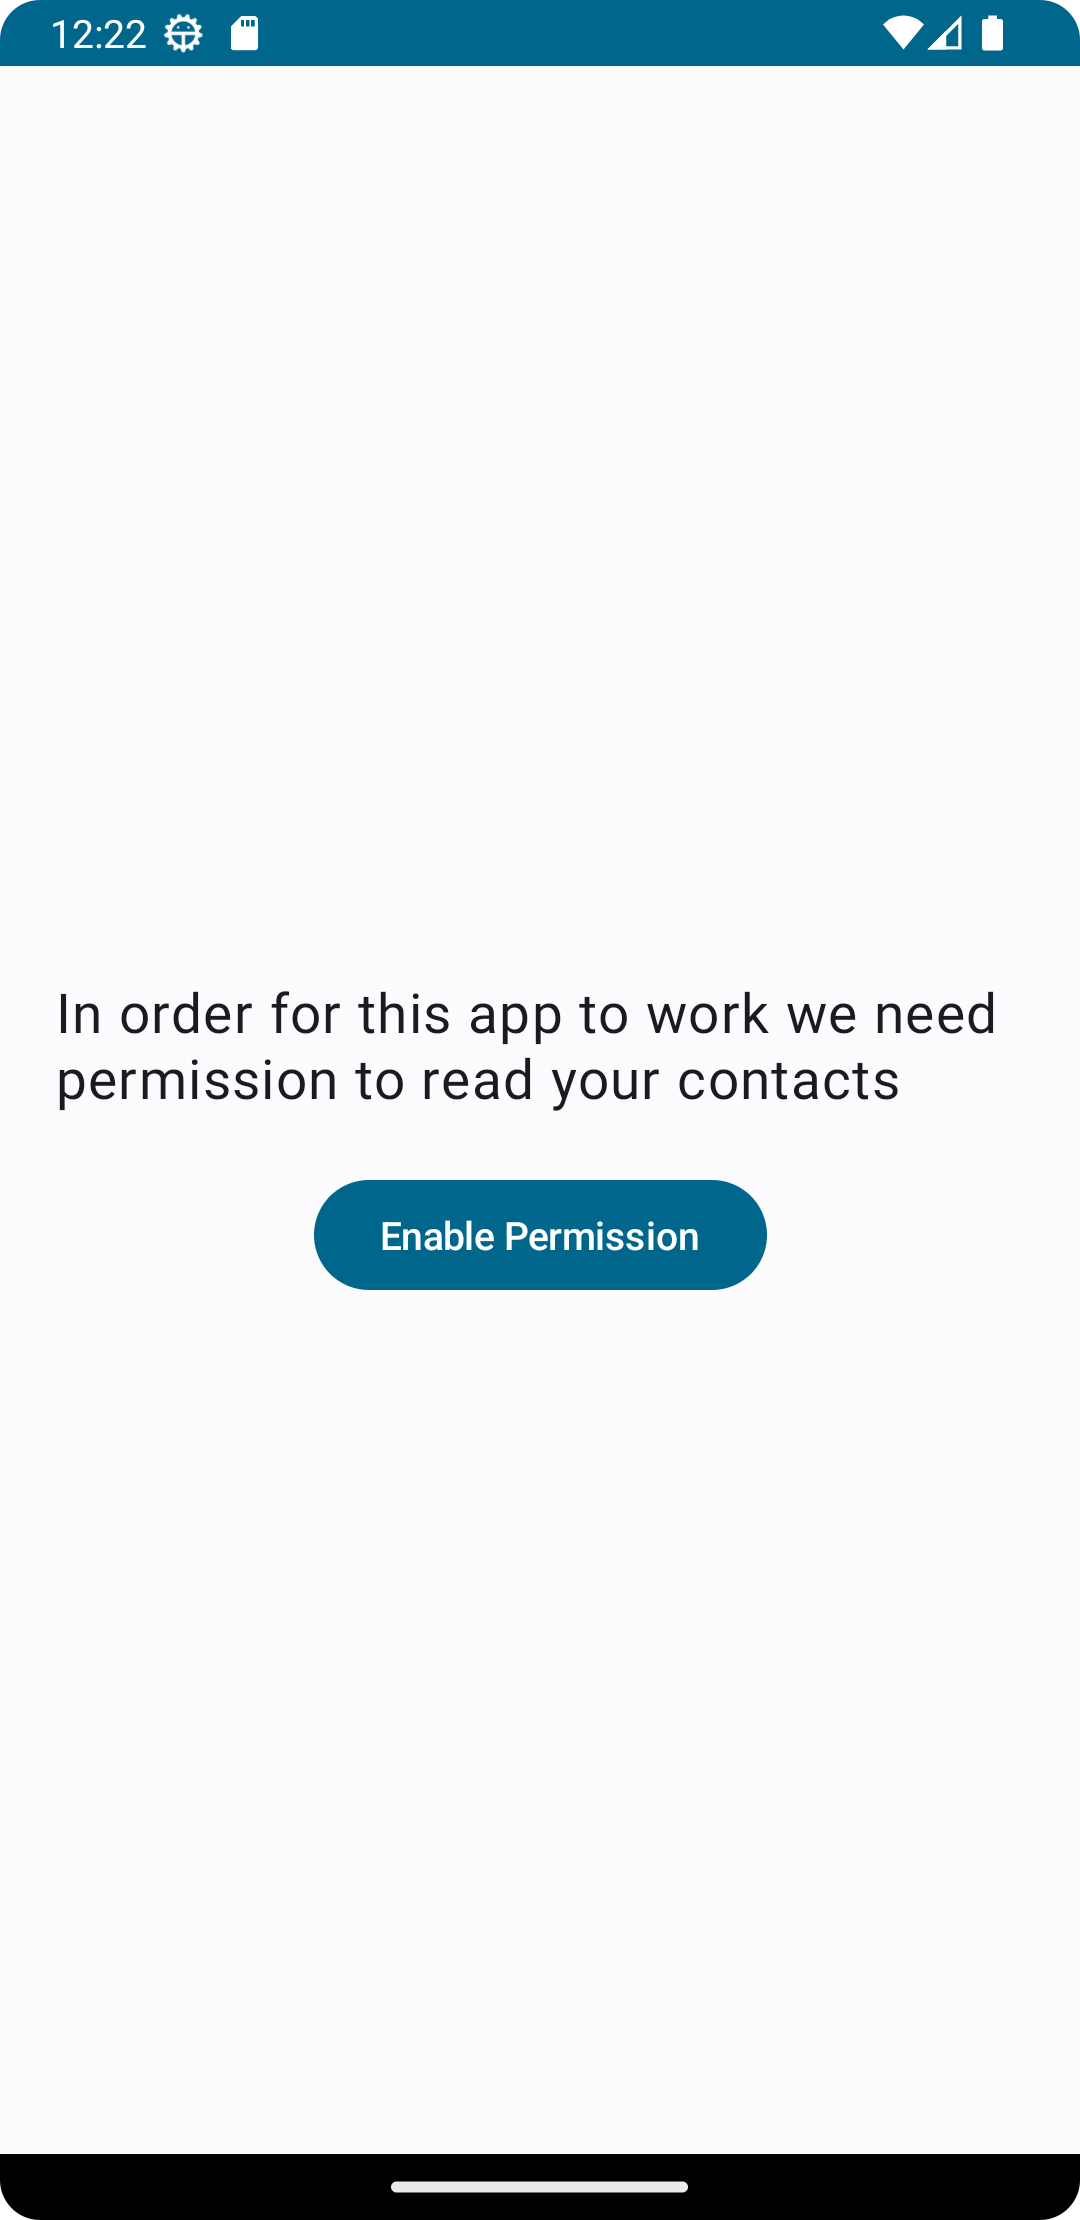
\includegraphics[trim={0cm 0cm 0 0cm}, width=0.4\textwidth]{./Chapter6/Figures/PermissionActivity}
	\caption{Permission Activity}
	\label{fig:PA}
\end{figure}


\subsection{Sign In}

The Sign-in Activity serves as the component for managing the user's authentication process, containing both logging in and registering in the service. Additionally, it ensures the secure storage of the user's token by leveraging the EncryptedSharedPreferences.

Upon launching the Sign-in Activity, users are presented with a user-friendly interface where they can enter their credentials or choose to register as a new user. The activity handles the input validation and securely communicates with the server-side authentication API.

Once the user's credentials are verified, the Sign-in Activity retrieves the authentication token from the server's response. To ensure the token's confidentiality, it is stored using the EncryptedSharedPreferences. This specialized SharedPreferences implementation employs encryption algorithms to protect sensitive data from unauthorized access.

By utilizing the EncryptedSharedPreferences, the Sign-in Activity safeguards the user's authentication token, preventing it from being tampered with or exposed. This secure storage mechanism provides an additional layer of protection for user data, mitigating the risks associated with unauthorized token access.


In addition, the Sign-in Activity incorporates an automatic phone number region retrieval feature by leveraging the Carrier information.

Because our app hasn't been deployed anywhere it is prompted to the user to choose whether he wants to use local data "Mock" or connect to an IP address - see \ref{SAIP}

Figures \ref{fig:SA1}, \ref{fig:SA2} illustrate the implemented activity.

\begin{figure}[!ht]
	\centering
	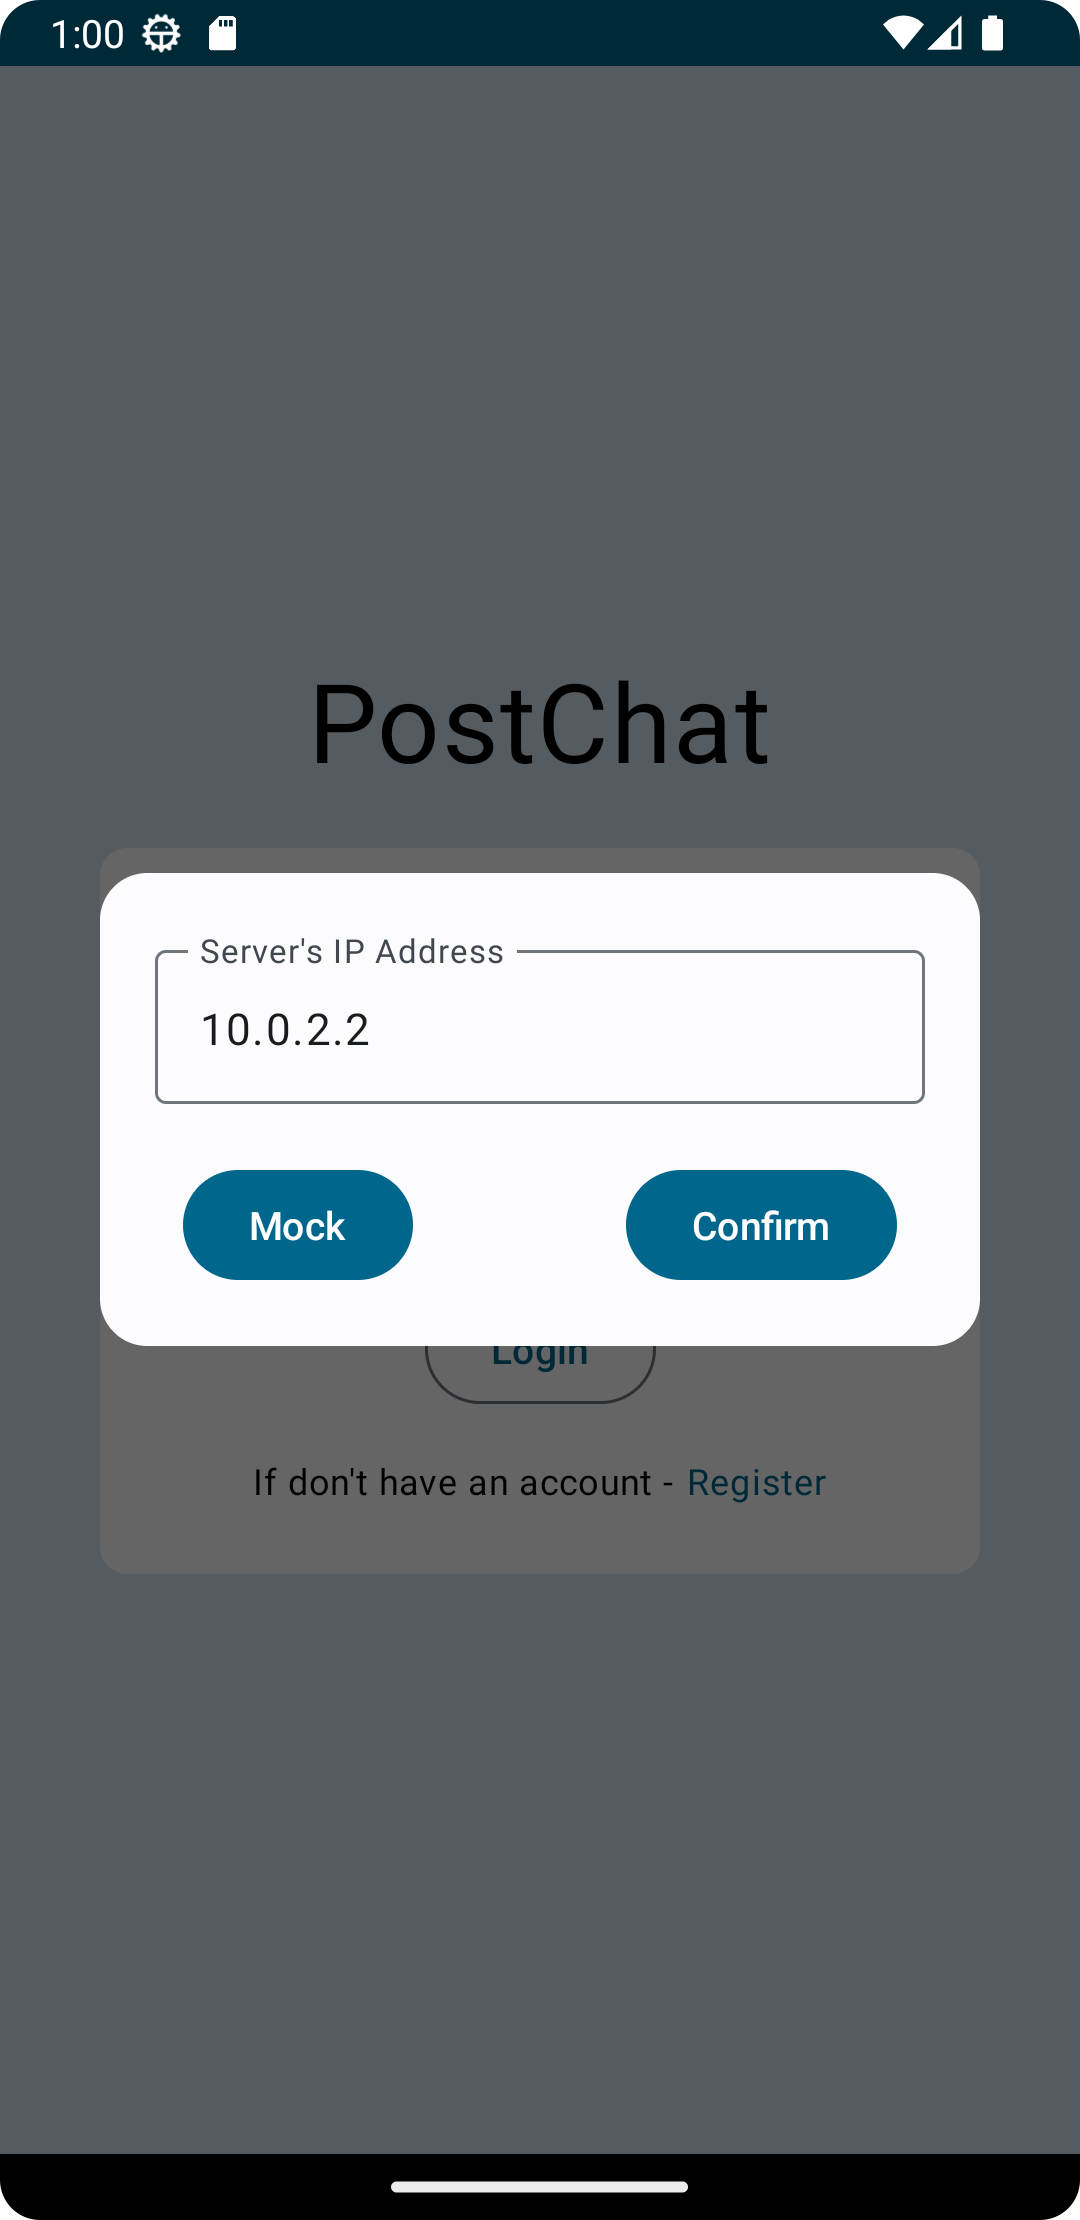
\includegraphics[trim={0cm -3cm 0 -3cm}, width=0.4\textwidth]{./Chapter6/Figures/SignInActivityIpAdress}
	\caption{Signin Activity}
	\label{fig:SAIP}
\end{figure}


\begin{figure}[!ht]
	\centering
	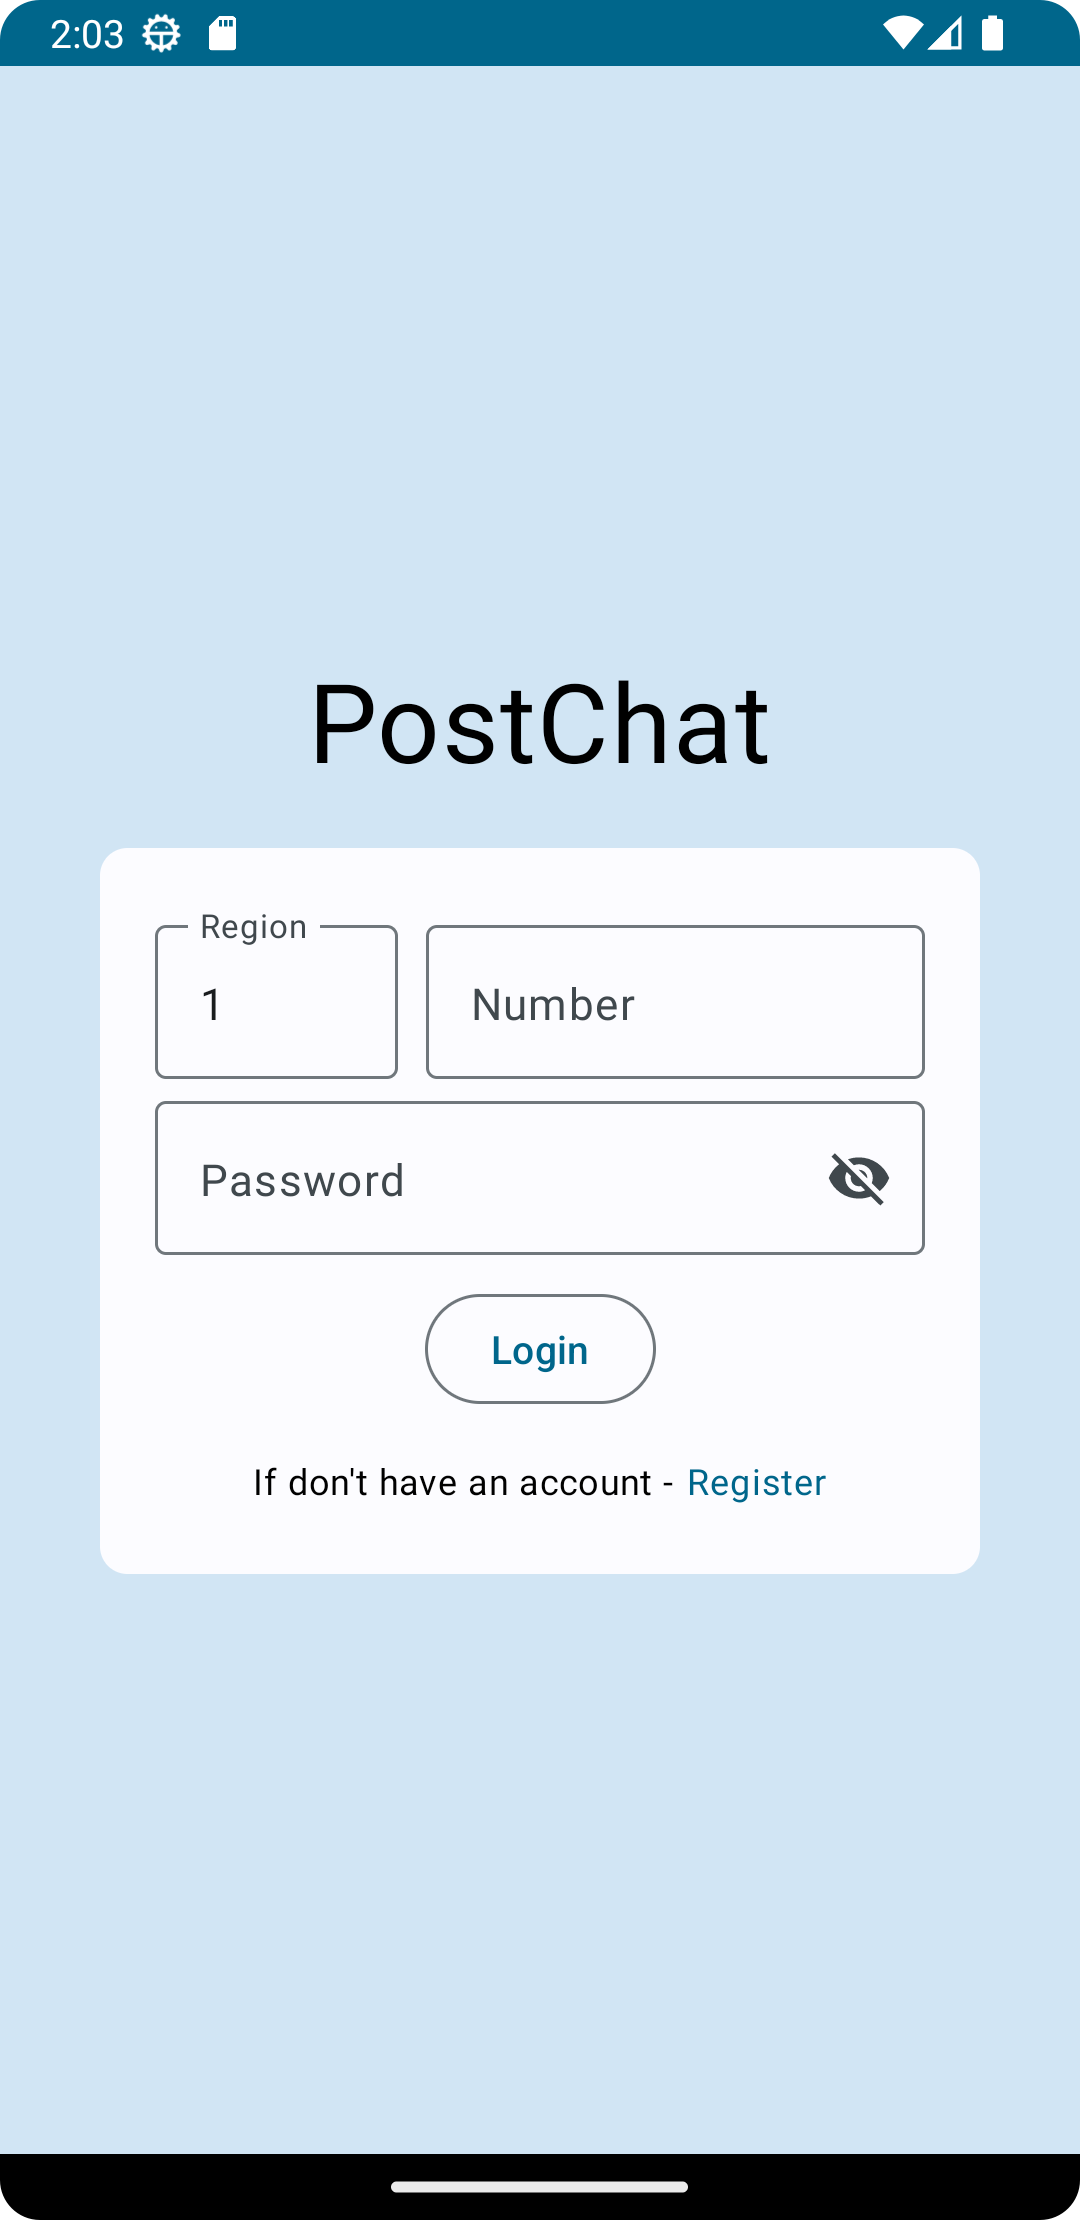
\includegraphics[trim={0cm -3cm 0 -3cm}, width=0.4\textwidth]{./Chapter6/Figures/SignInActivityLogin}
	\caption{Signin Activity}
	\label{fig:SA1}
\end{figure}


It also does local verification's to user's input. Password and Phone Number validations are done using Google's API.

\begin{figure}[!ht]
	\centering
	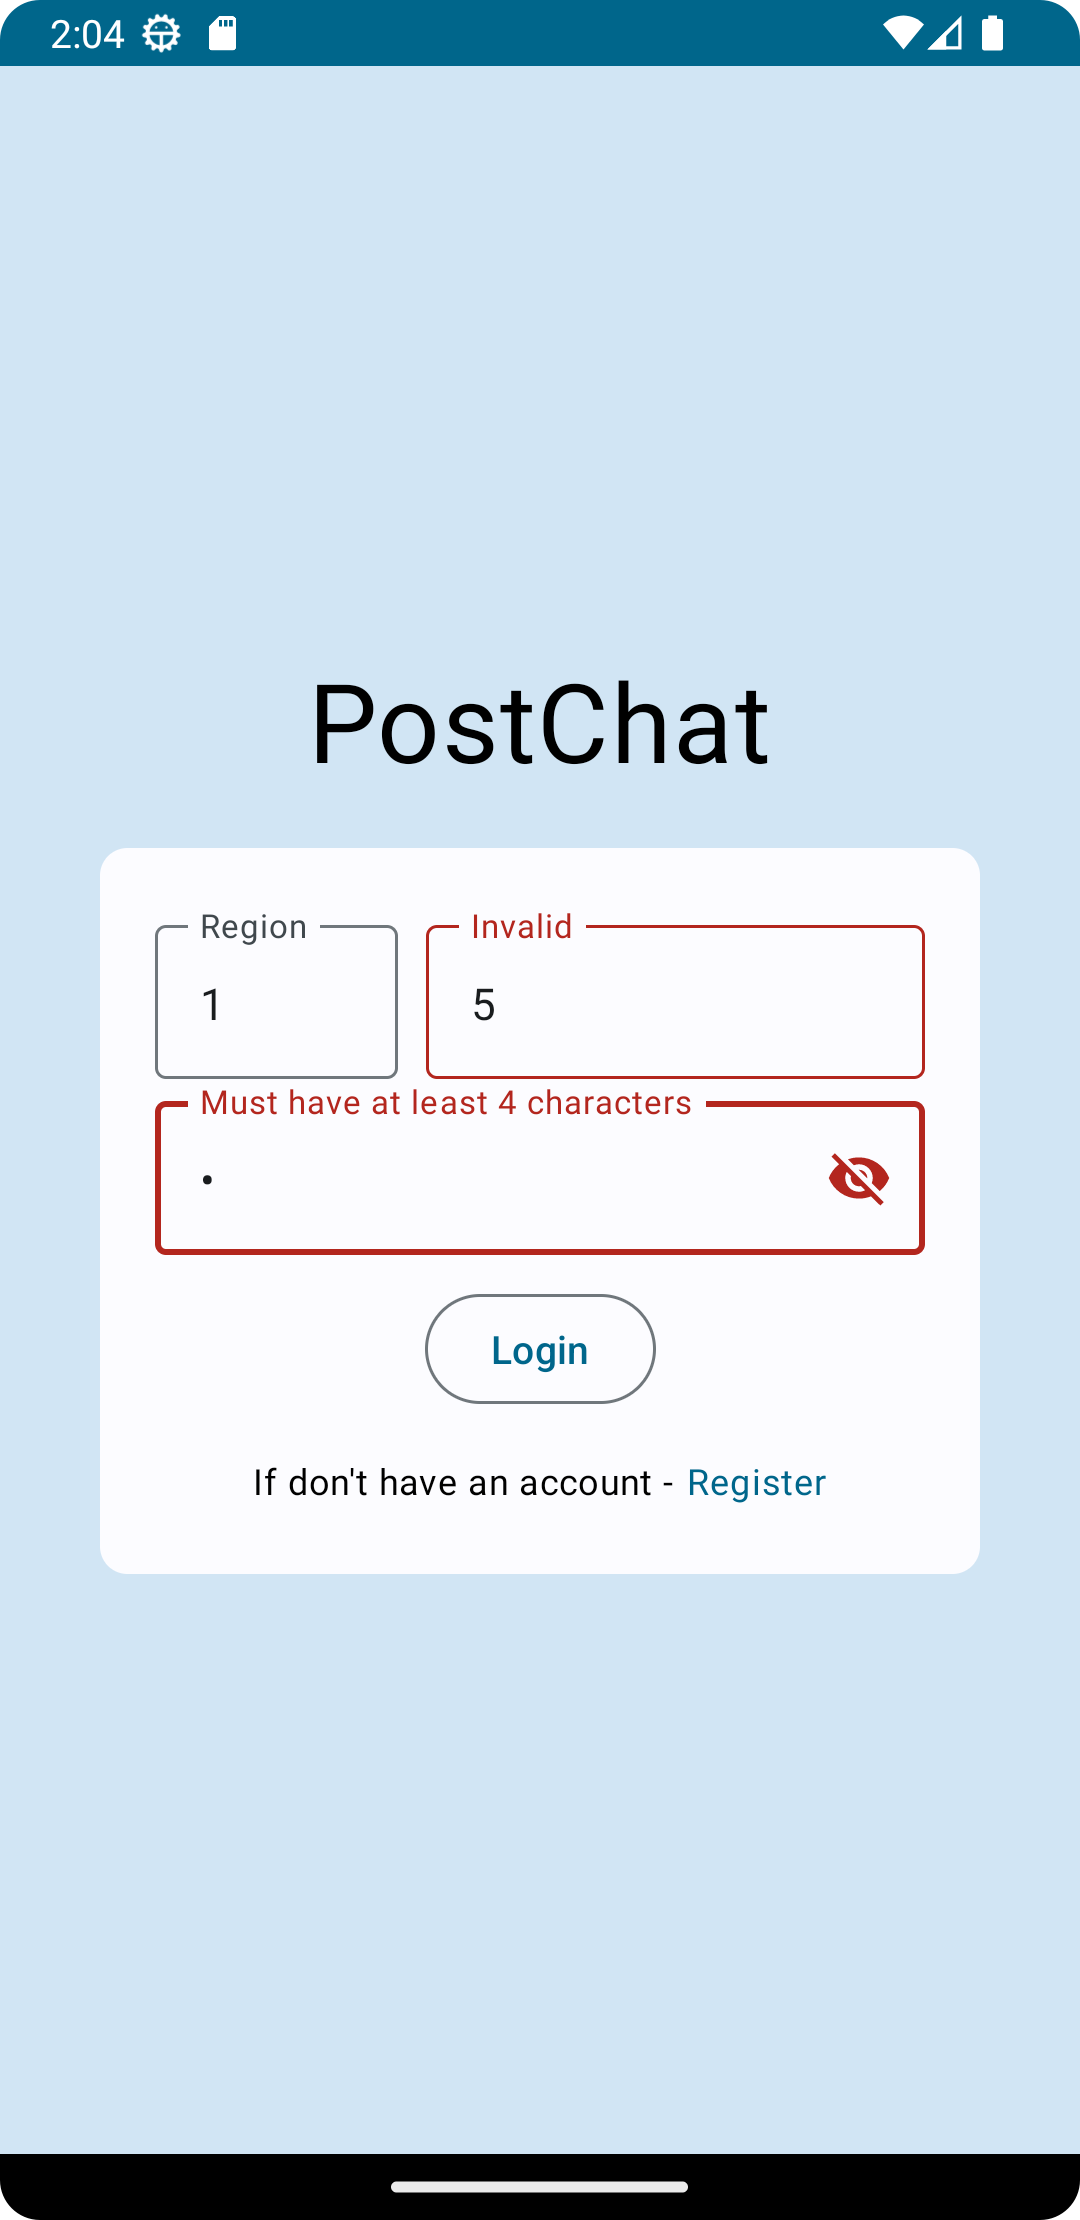
\includegraphics[trim={0cm -3cm 0 -3cm}, width=0.4\textwidth]{./Chapter6/Figures/SignInActivityErrors}
	\caption{Signin Activity invalid password size}
	\label{fig:SA2}
\end{figure}


\subsection{Home}
The Home Activity serves as a central hub for connecting to the web API and retrieving essential information related to registered users, messages, and chats. Its primary purpose is to display all chats in a user-friendly manner, with the chats ordered based on the most recent message received.

By establishing a connection with the web API, the Home Activity can fetch the necessary data to populate the chat interface. It retrieves information about registered users, ensuring that the appropriate user profiles are displayed within the chat list. Additionally, it retrieves messages associated with each chat, allowing users to view their conversation history.

The Home Activity organizes the chats in a manner that prioritizes the most recent interactions. By ordering the chats based on the last message received, users can quickly identify and access their most recent conversations.

Moreover, the Home Activity provides intuitive controls and a simple interface, users can create new chat groups, within a button.

Figure~\ref{fig:HA1} illustrate the implemented activity.

\begin{figure}[!ht]
	\centering
	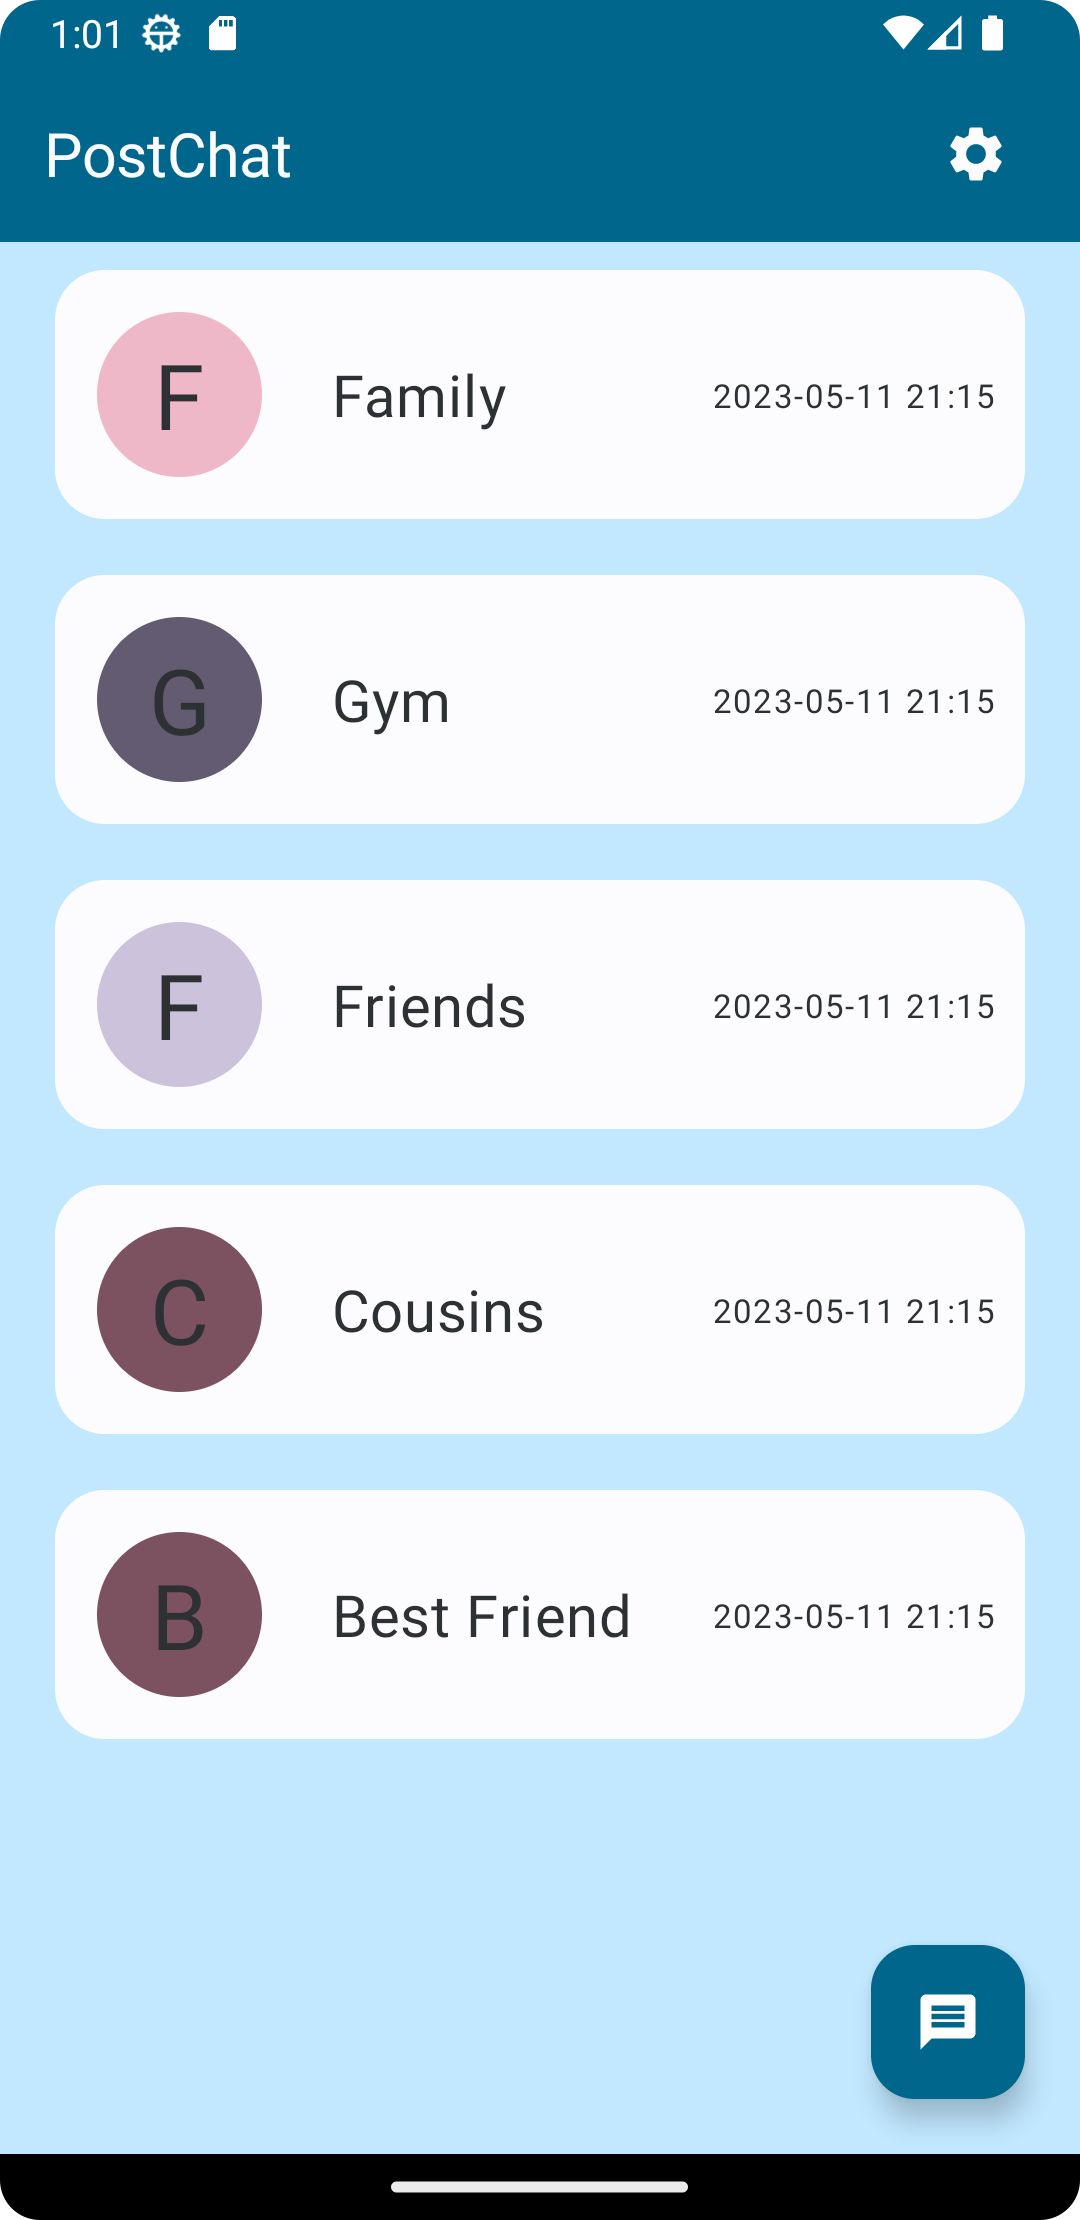
\includegraphics[trim={0cm -3cm 0 -3cm}, width=0.4\textwidth]{./Chapter6/Figures/HomeActivity}
	\caption{Home Activity}
	\label{fig:HA1}
\end{figure}


\subsection{Create Chat}
The CreateChat activity searches for the users stored in the local database and lets you pick the phone numbers you want to add to the chat. Every chat needs a name so a popup dialog input message shows when clicking the check button.

Figures \ref{fig:CCA1} and \ref{fig:CCA2} illustrate the implemented activity.


\begin{figure}[!ht]
	\centering
	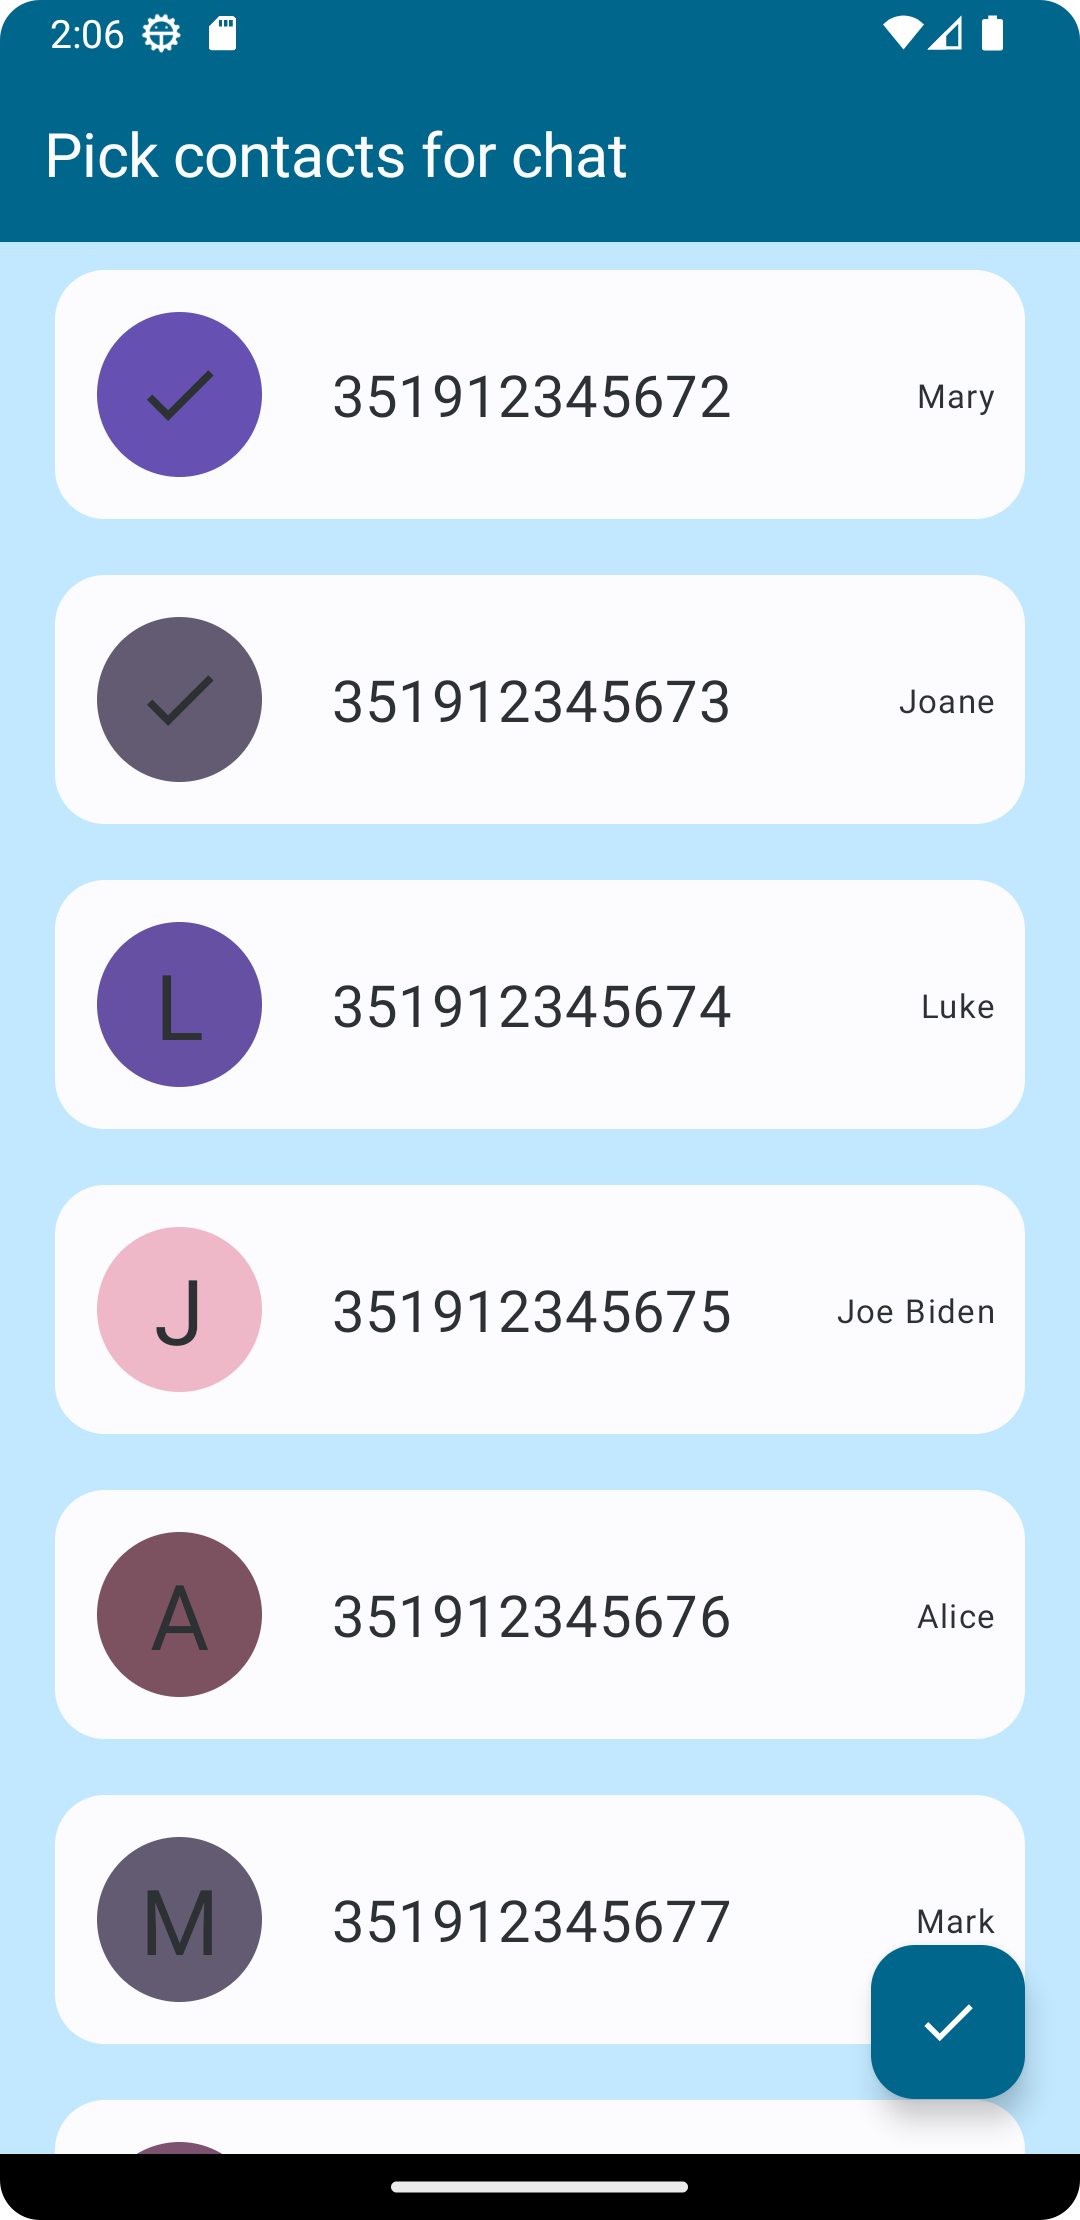
\includegraphics[trim={0cm -3cm 0 -3cm}, width=0.4\textwidth]{./Chapter6/Figures/CreateChatActivityPickContacts}
	\caption{CreateChat Activity}
	\label{fig:CCA1}
\end{figure}


\begin{figure}[!ht]
	\centering
	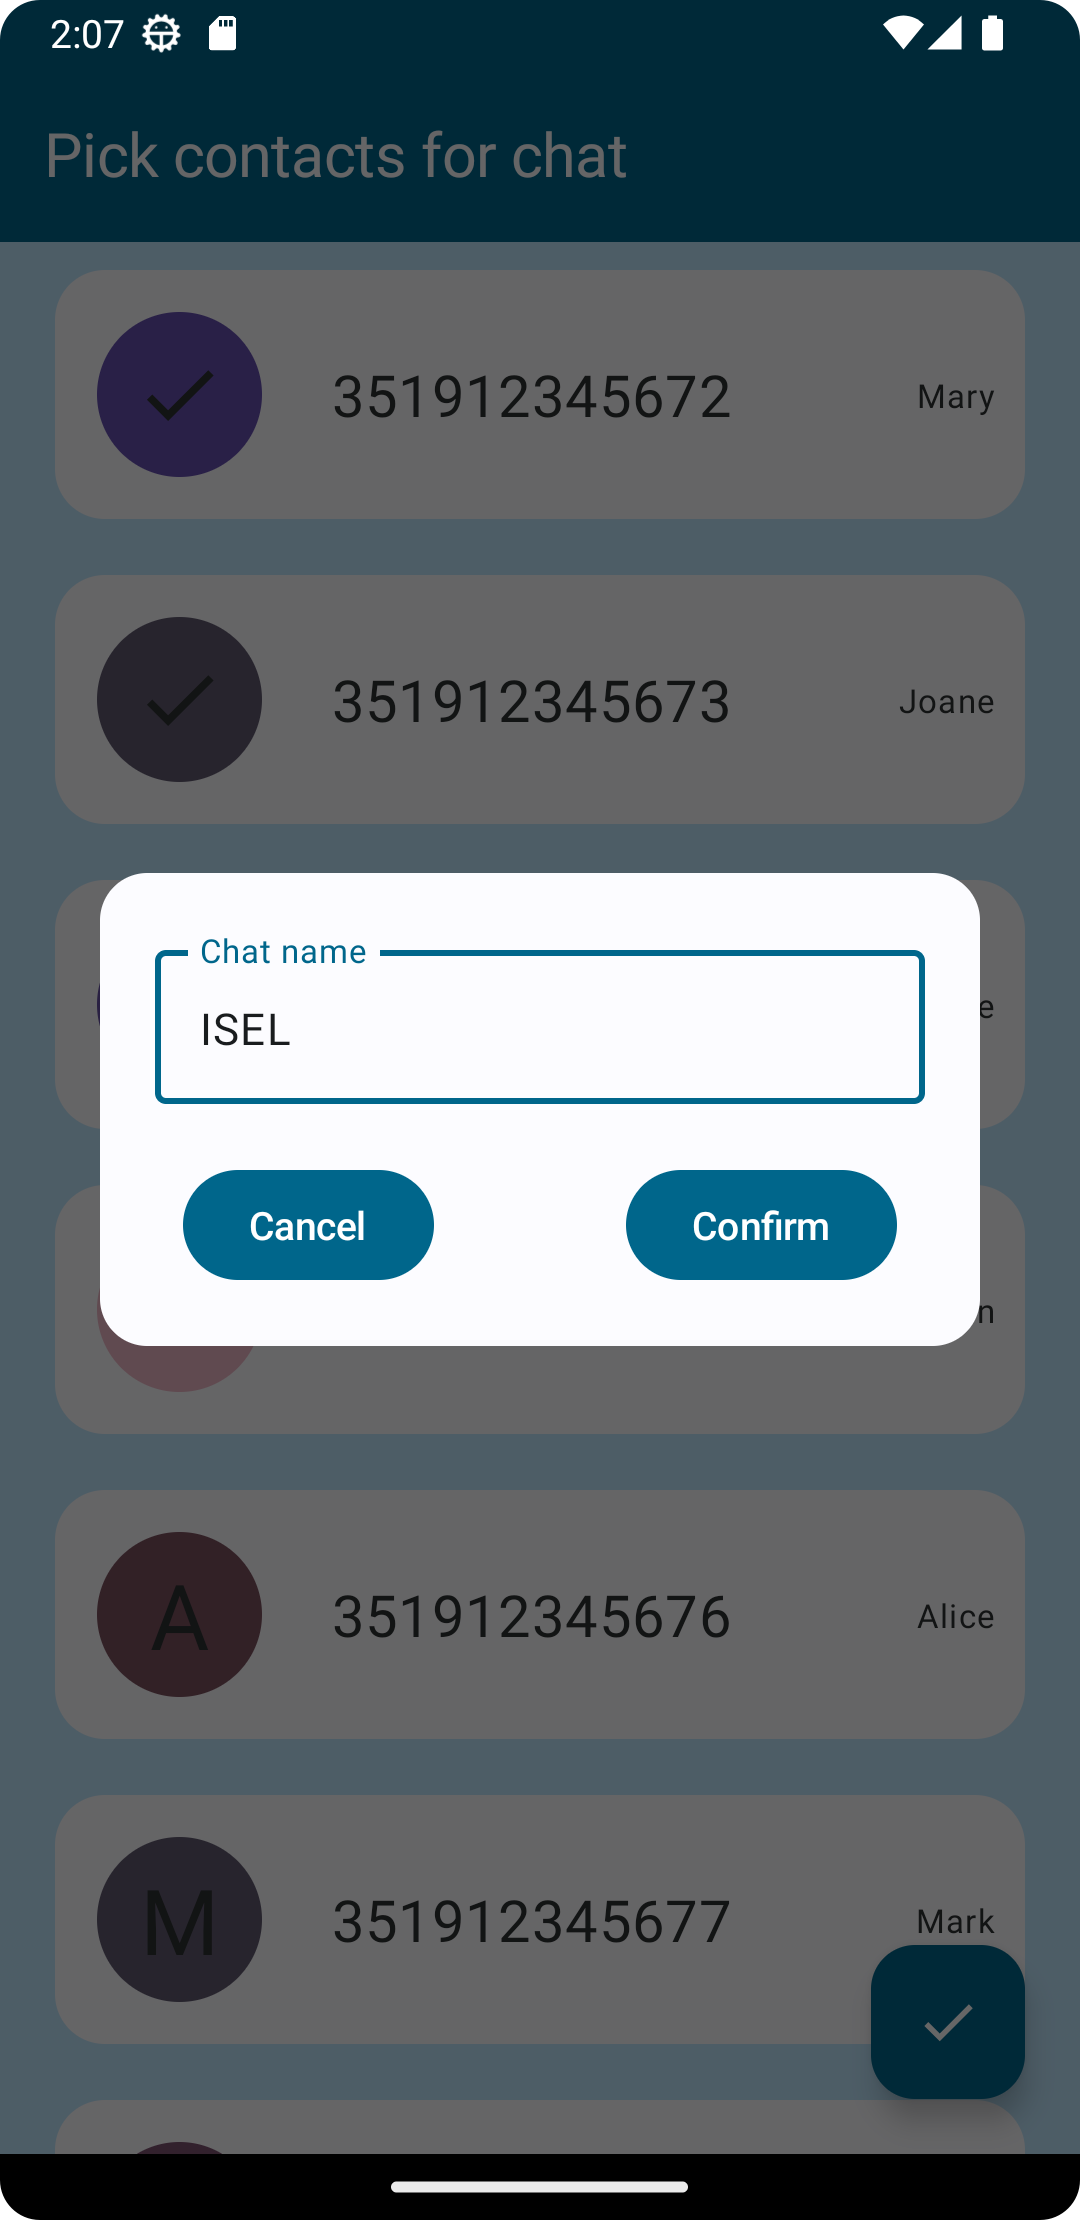
\includegraphics[trim={0cm -3cm 0 -3cm}, width=0.4\textwidth]{./Chapter6/Figures/CreateChatActivityName}
	\caption{CreateChat Activity name prompt}
	\label{fig:CCA2}
\end{figure}

\subsection{Chat View}
The Chat activity obtains the information about the current chat messages. 
It displays the postcards in order by the timestamp and above the same it shows the number from the person that sent the message. In the future this will be changed to query users in the local database and get their name.  

Figures \ref{fig:CVA1}, \ref{fig:CVA2} , \ref{fig:CVA3} and \ref{fig:CVA4} illustrate the implemented activity.

\begin{figure}[!ht]
	\centering
	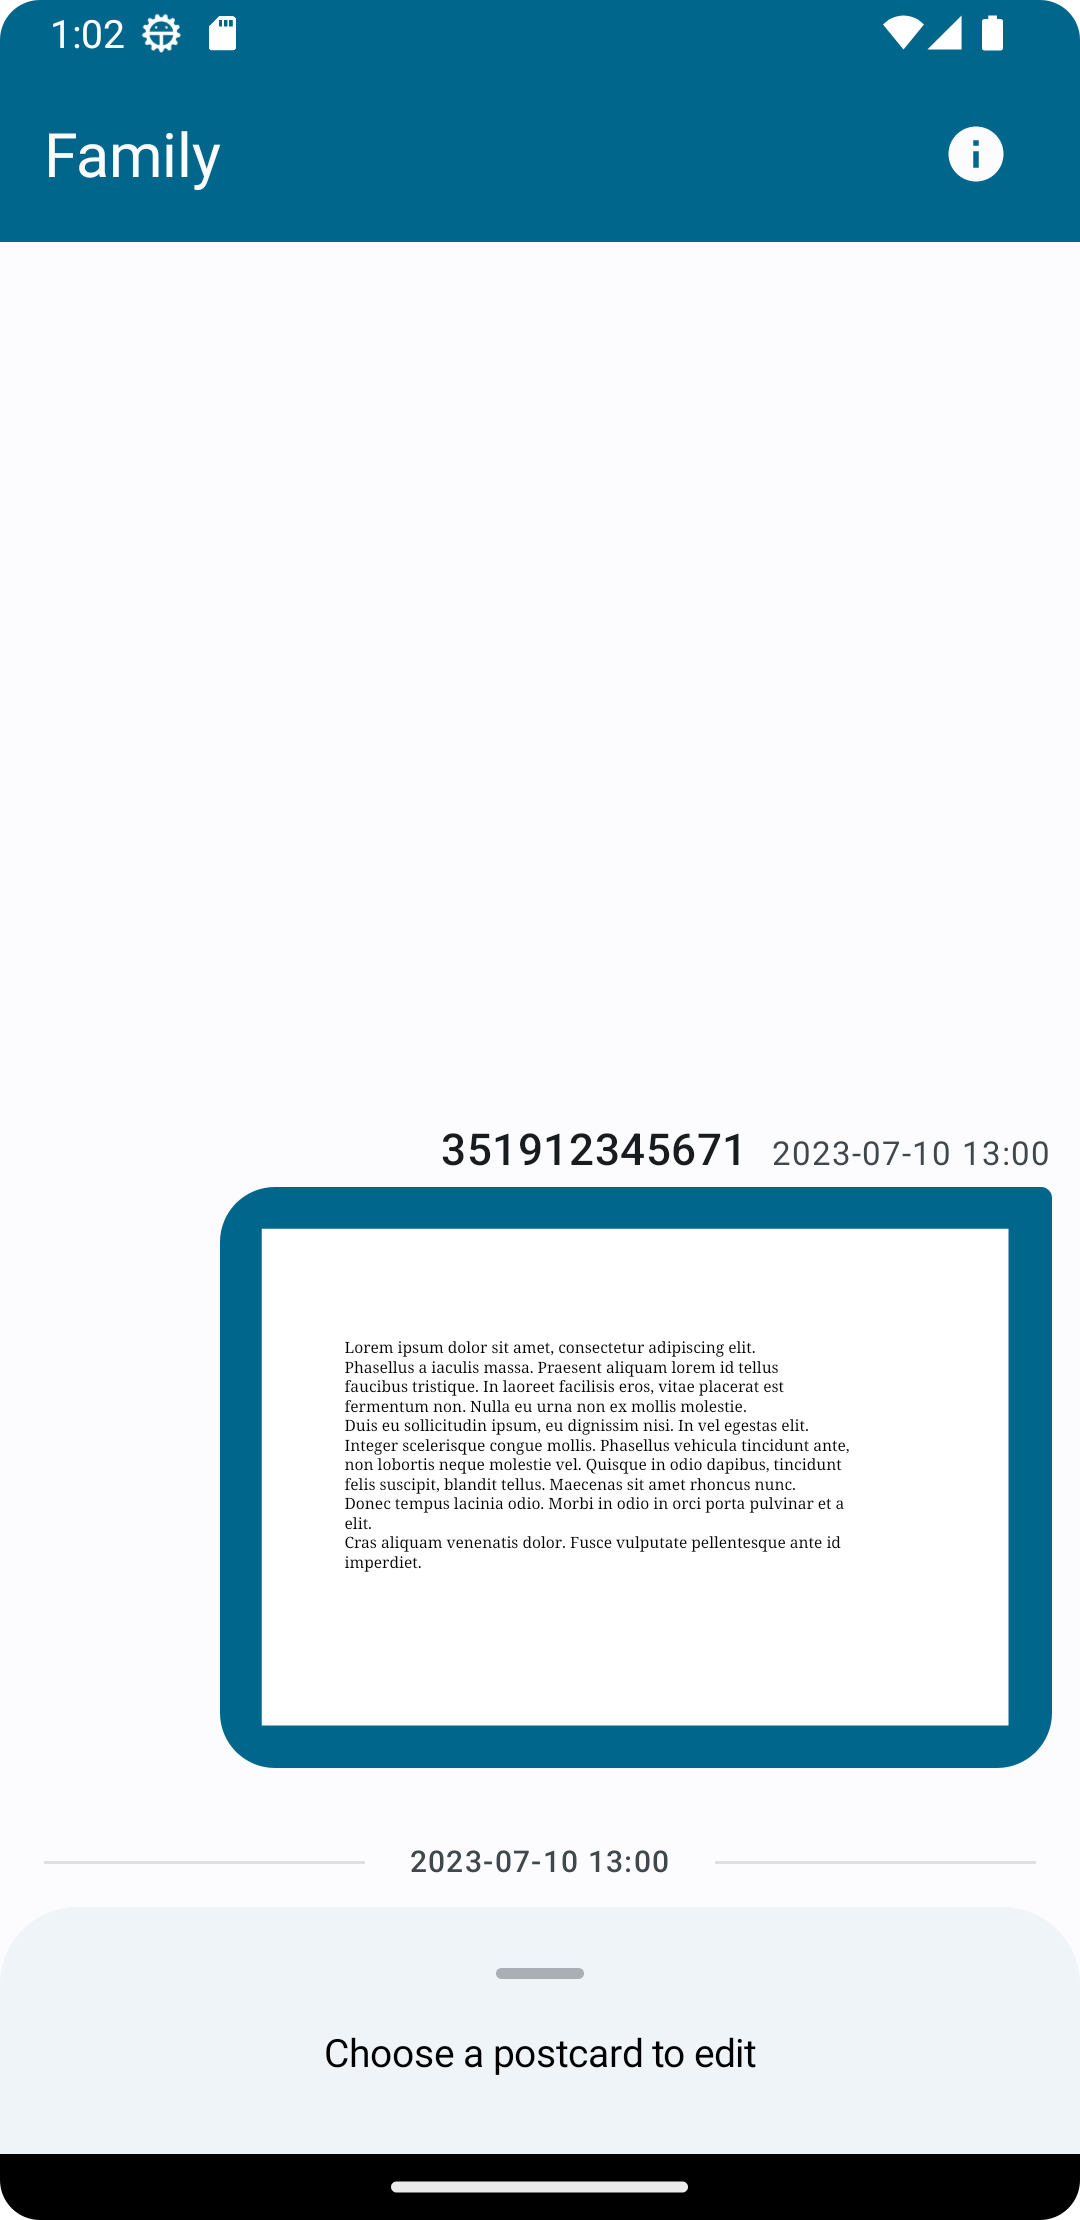
\includegraphics[trim={0cm -3cm 0 -3cm}, width=0.4\textwidth]{./Chapter6/Figures/ChatActivity}
	\caption{Chat Activity}
	\label{fig:CVA1}
\end{figure}


\begin{figure}[!ht]
	\centering
	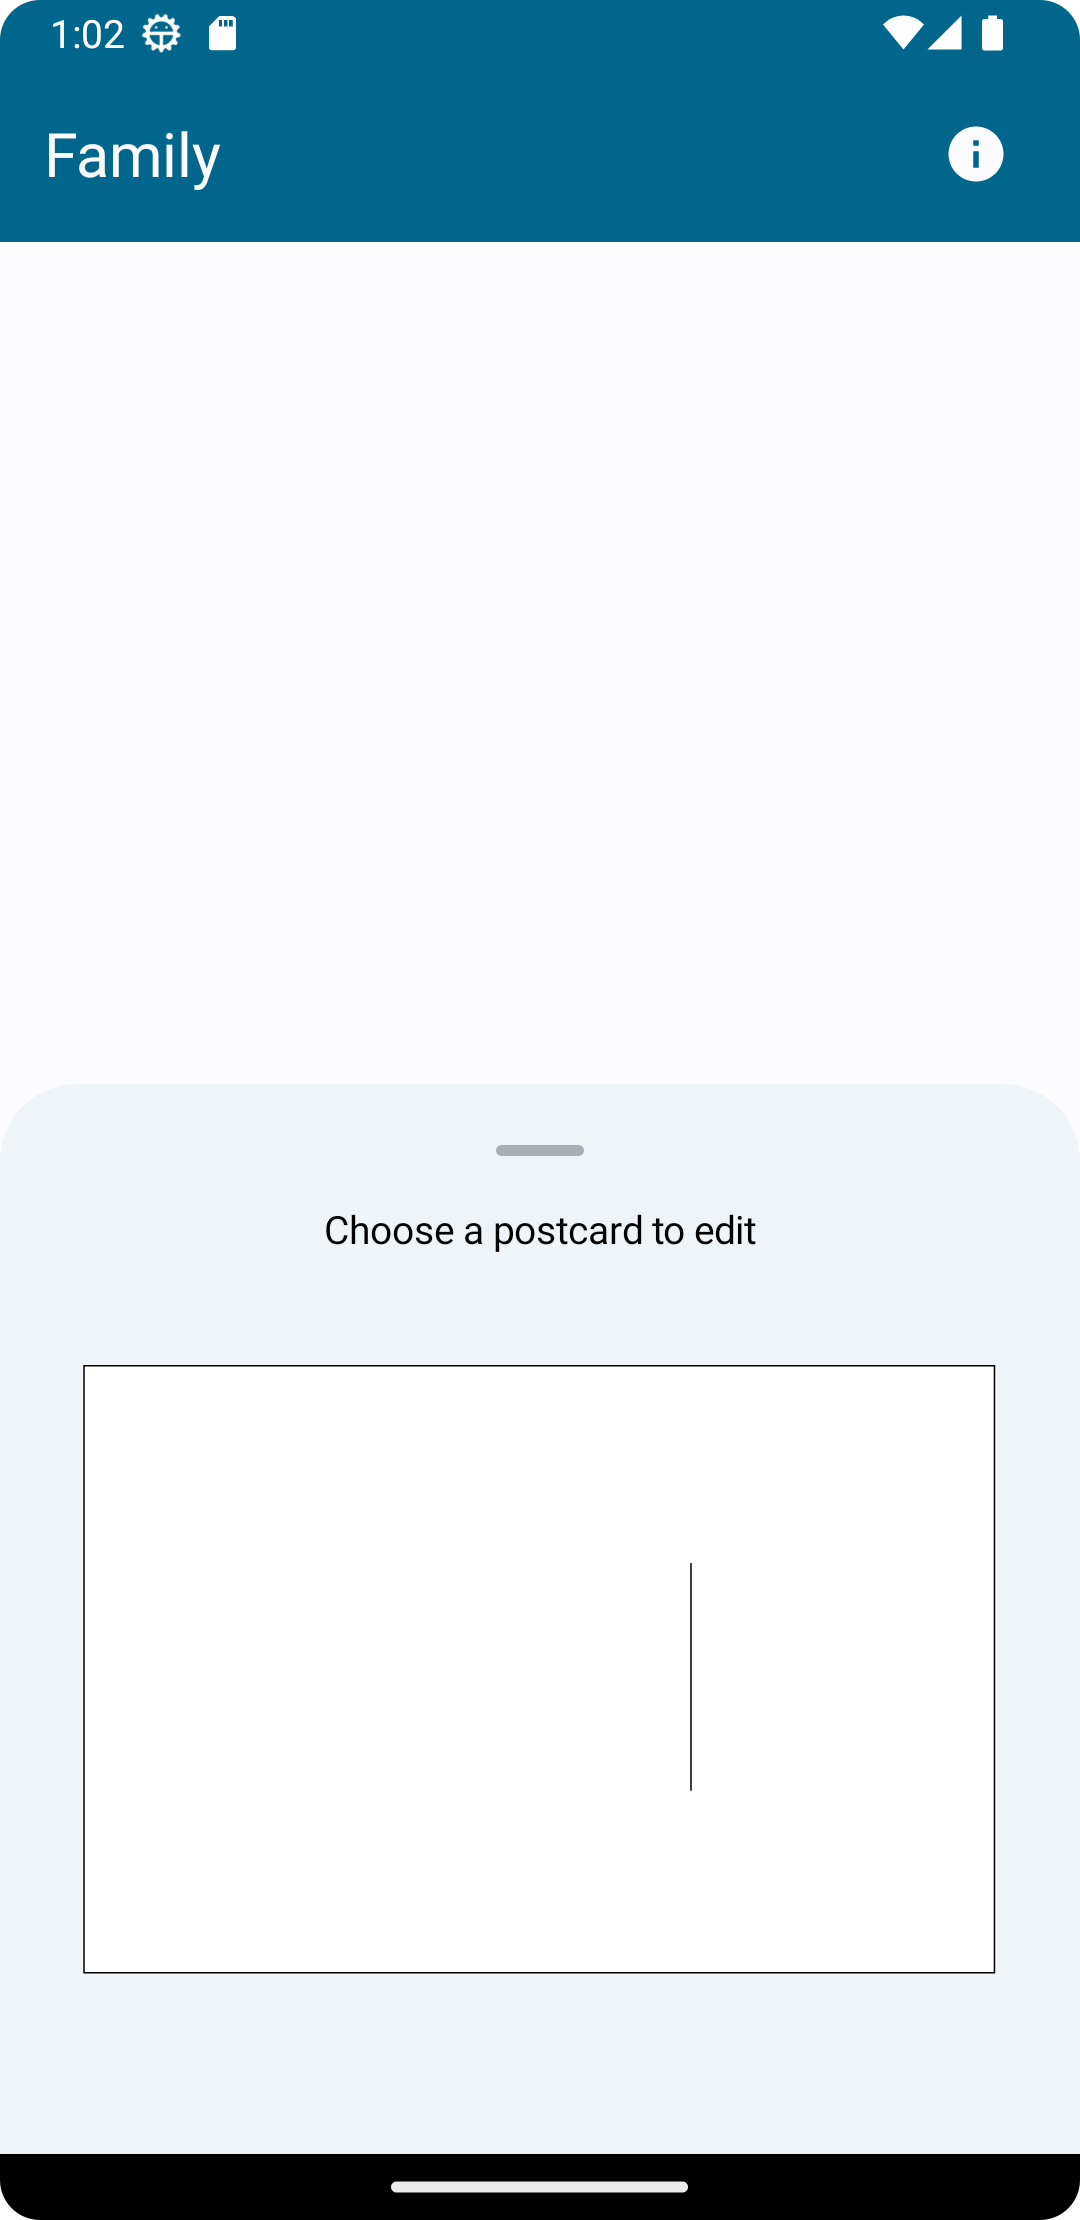
\includegraphics[trim={0cm -3cm 0 -3cm}, width=0.4\textwidth]{./Chapter6/Figures/ChatActivityShowPostcards}
	\caption{Chat Activity bottom templates list}
	\label{fig:CVA2}
\end{figure}


\begin{figure}[!ht]
	\centering
	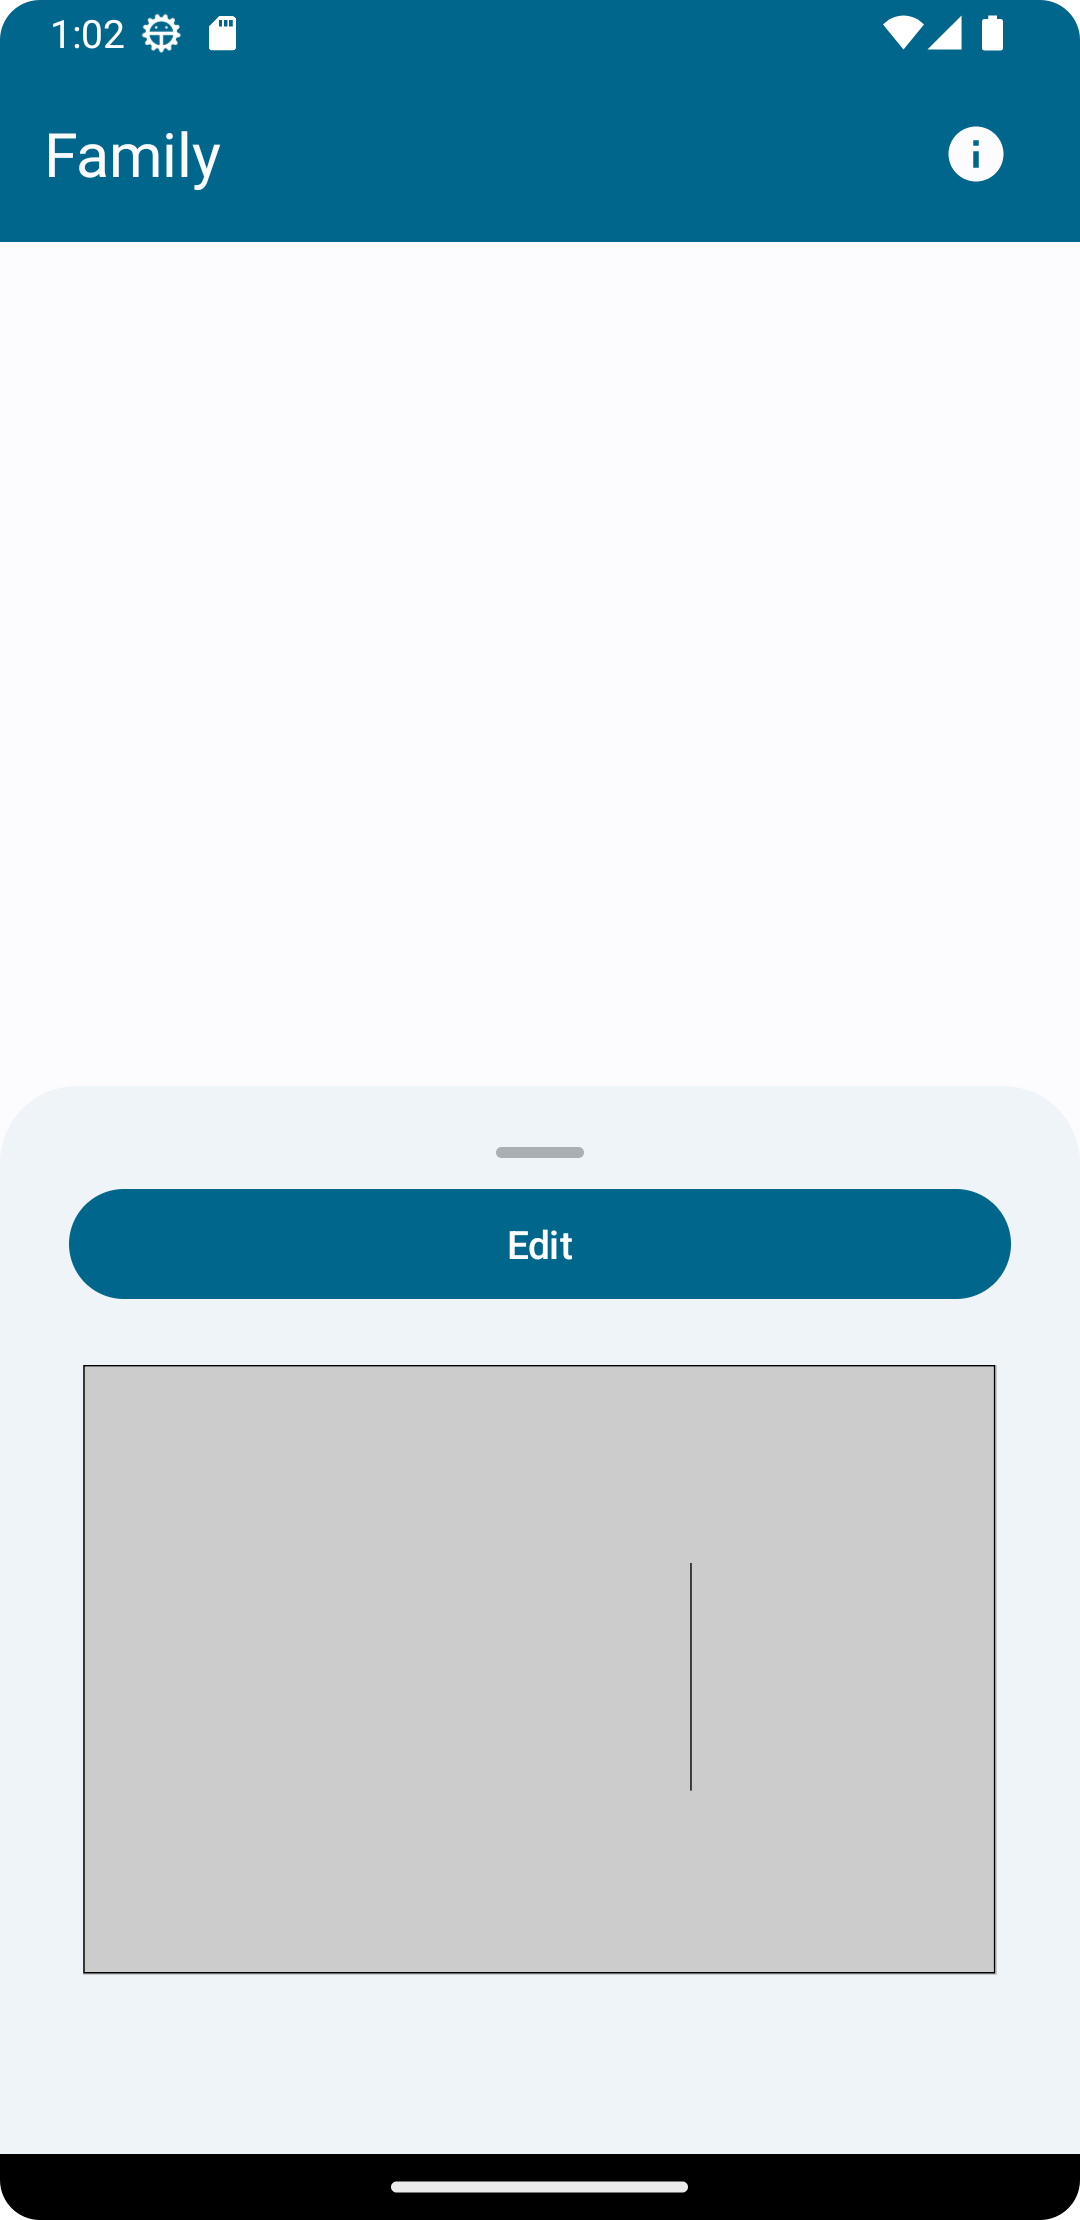
\includegraphics[trim={0cm -3cm 0 -3cm}, width=0.4\textwidth]{./Chapter6/Figures/ChatActivityPickPostcard}
	\caption{Chat Activity pick template}
	\label{fig:CVA3}
\end{figure}

On clicking the edit button the user is sent to the Draw Activity.

\begin{figure}[!ht]
	\centering
	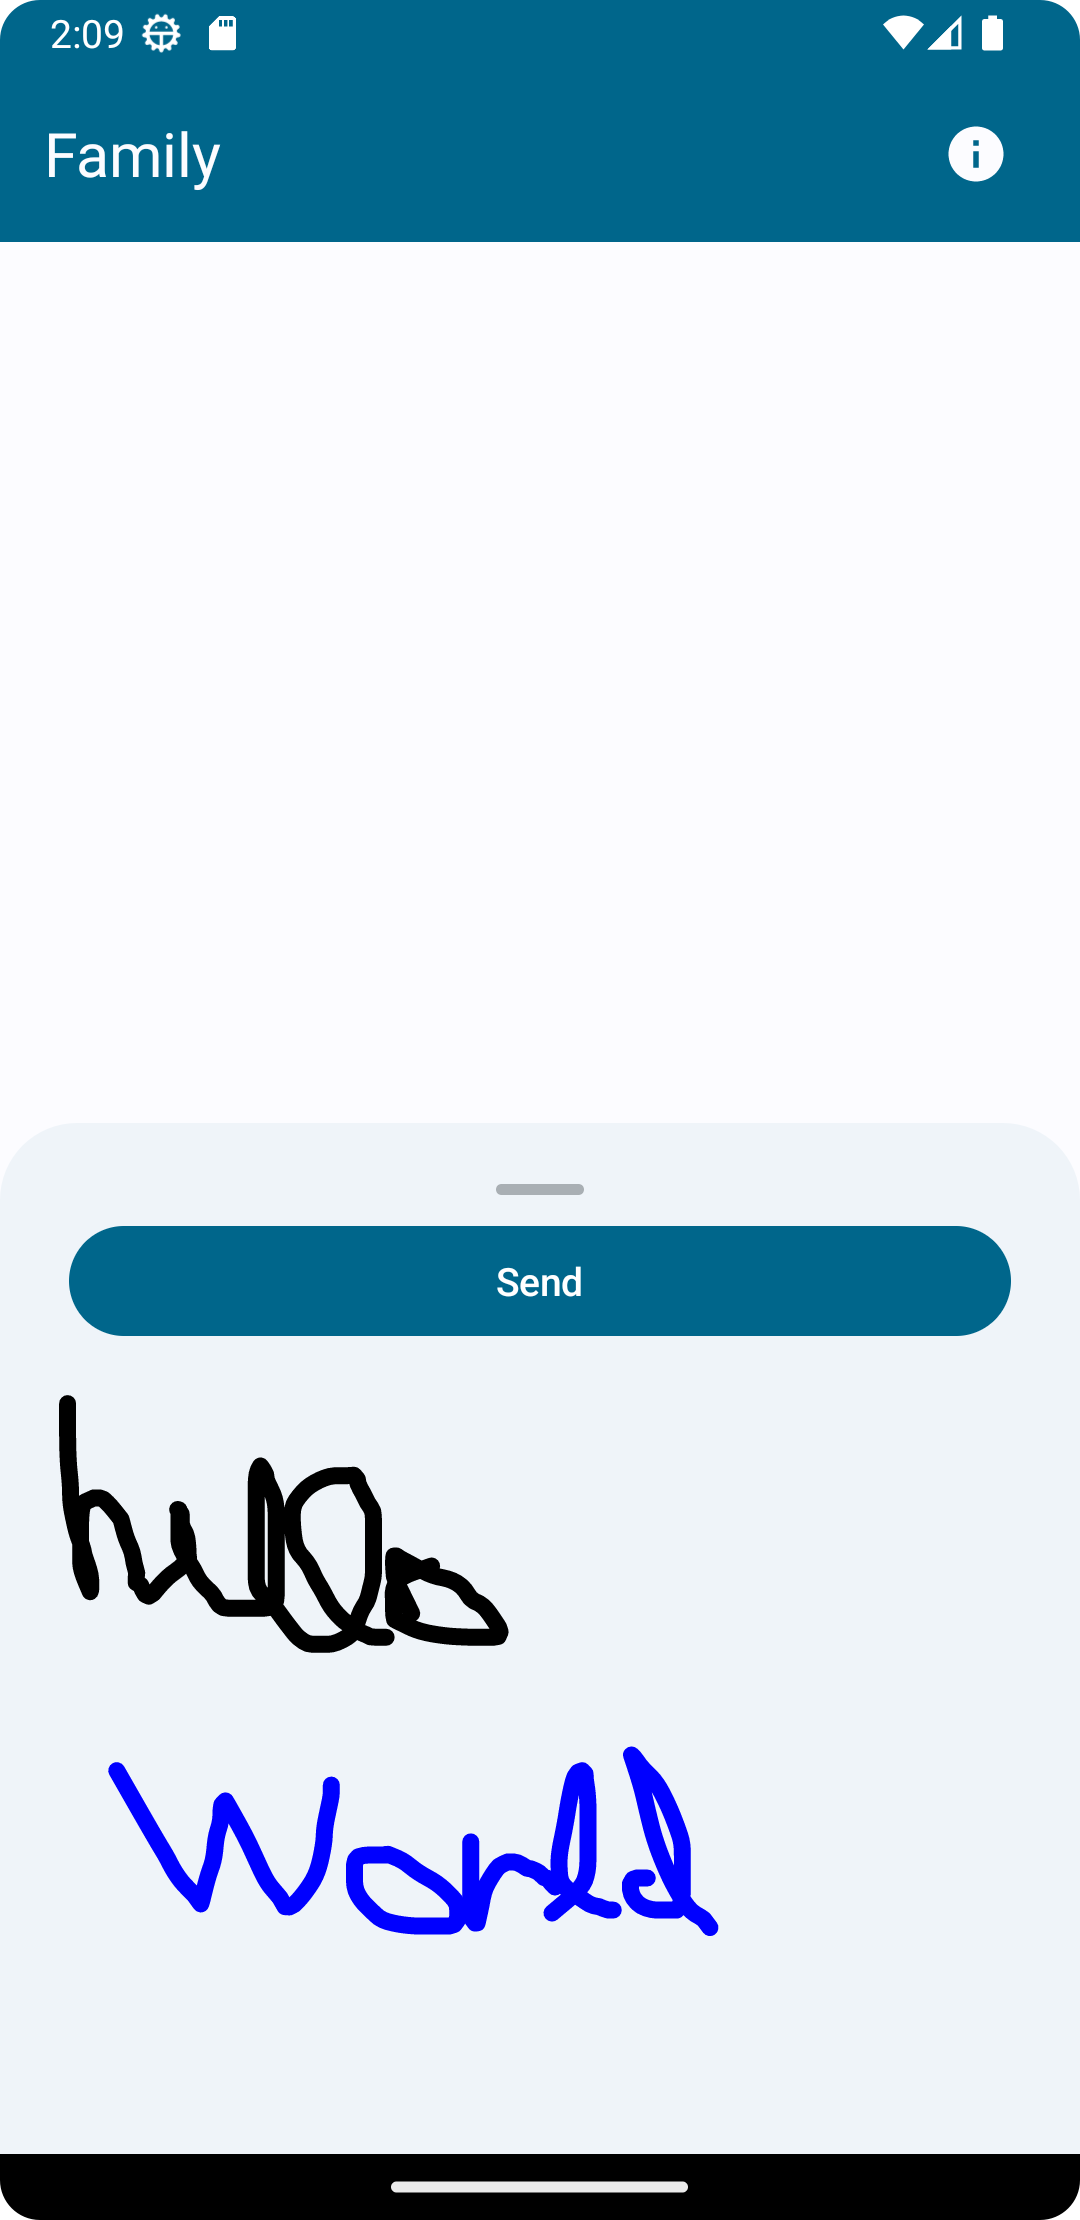
\includegraphics[trim={0cm -3cm 0 -3cm}, width=0.4\textwidth]{./Chapter6/Figures/ChatActivityPreview}
	\caption{CreateChat preview postcard}
	\label{fig:CVA4}
\end{figure}


\begin{figure}[!ht]
	\centering
	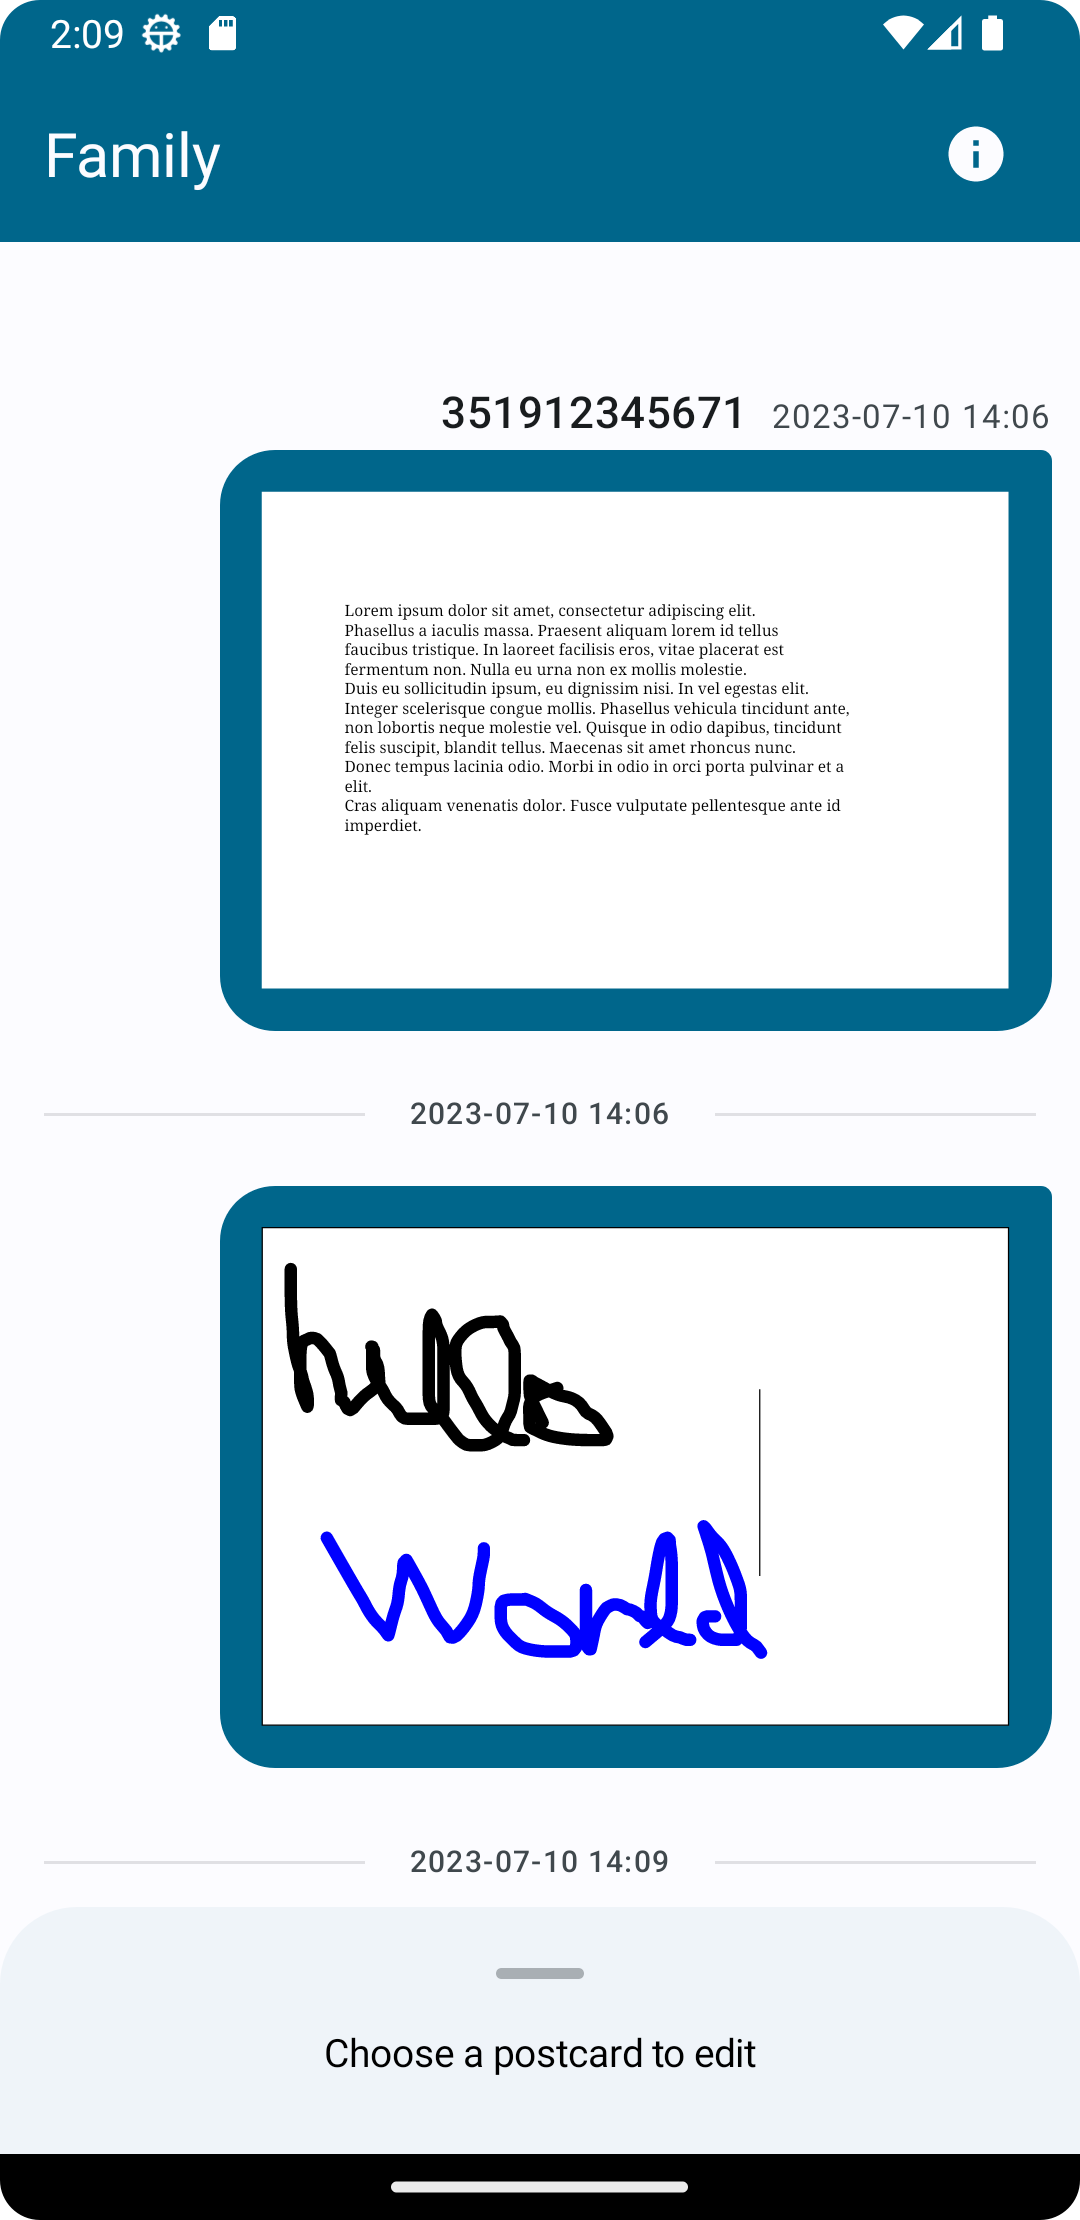
\includegraphics[trim={0cm -3cm 0 -3cm}, width=0.4\textwidth]{./Chapter6/Figures/ChatActivityUpdated}
	\caption{CreateChat postcard sent}
	\label{fig:CVA4}
\end{figure}



\subsection{Draw Postcard}
The Draw activity plays a crucial role in allowing users to edit and personalize a postcard using the Canvas. It involves implementing complex code to enable features such as drawing, zooming, and saving the postcard.

The challenge in implementing drawing and zoom features arise from the absence of a built-in two-finger zoom and one-finger touch draw function in the compose toolkit. To overcome this limitation, an in-depth analysis of the compose toolkit's inner code was conducted. By examining the underlying mechanisms of the compose toolkit, the necessary functionality for drawing and zooming was achieved.

To facilitate the saving of the canvas, a list is used to store the properties of each path. Each path property consists of the actual path data and the stroke style applied to it. When the canvas needs to be saved, the application iterates through each path in the list and generates an SVG file.

During the SVG file creation process, the application adds the necessary path movements and stroke styles to accurately represent each drawn path. This ensures that the saved SVG file faithfully represents the visual appearance of the canvas.

Figures \ref{fig:DA1} illustrate the implemented activity.



\begin{figure}[!ht]
	\centering
	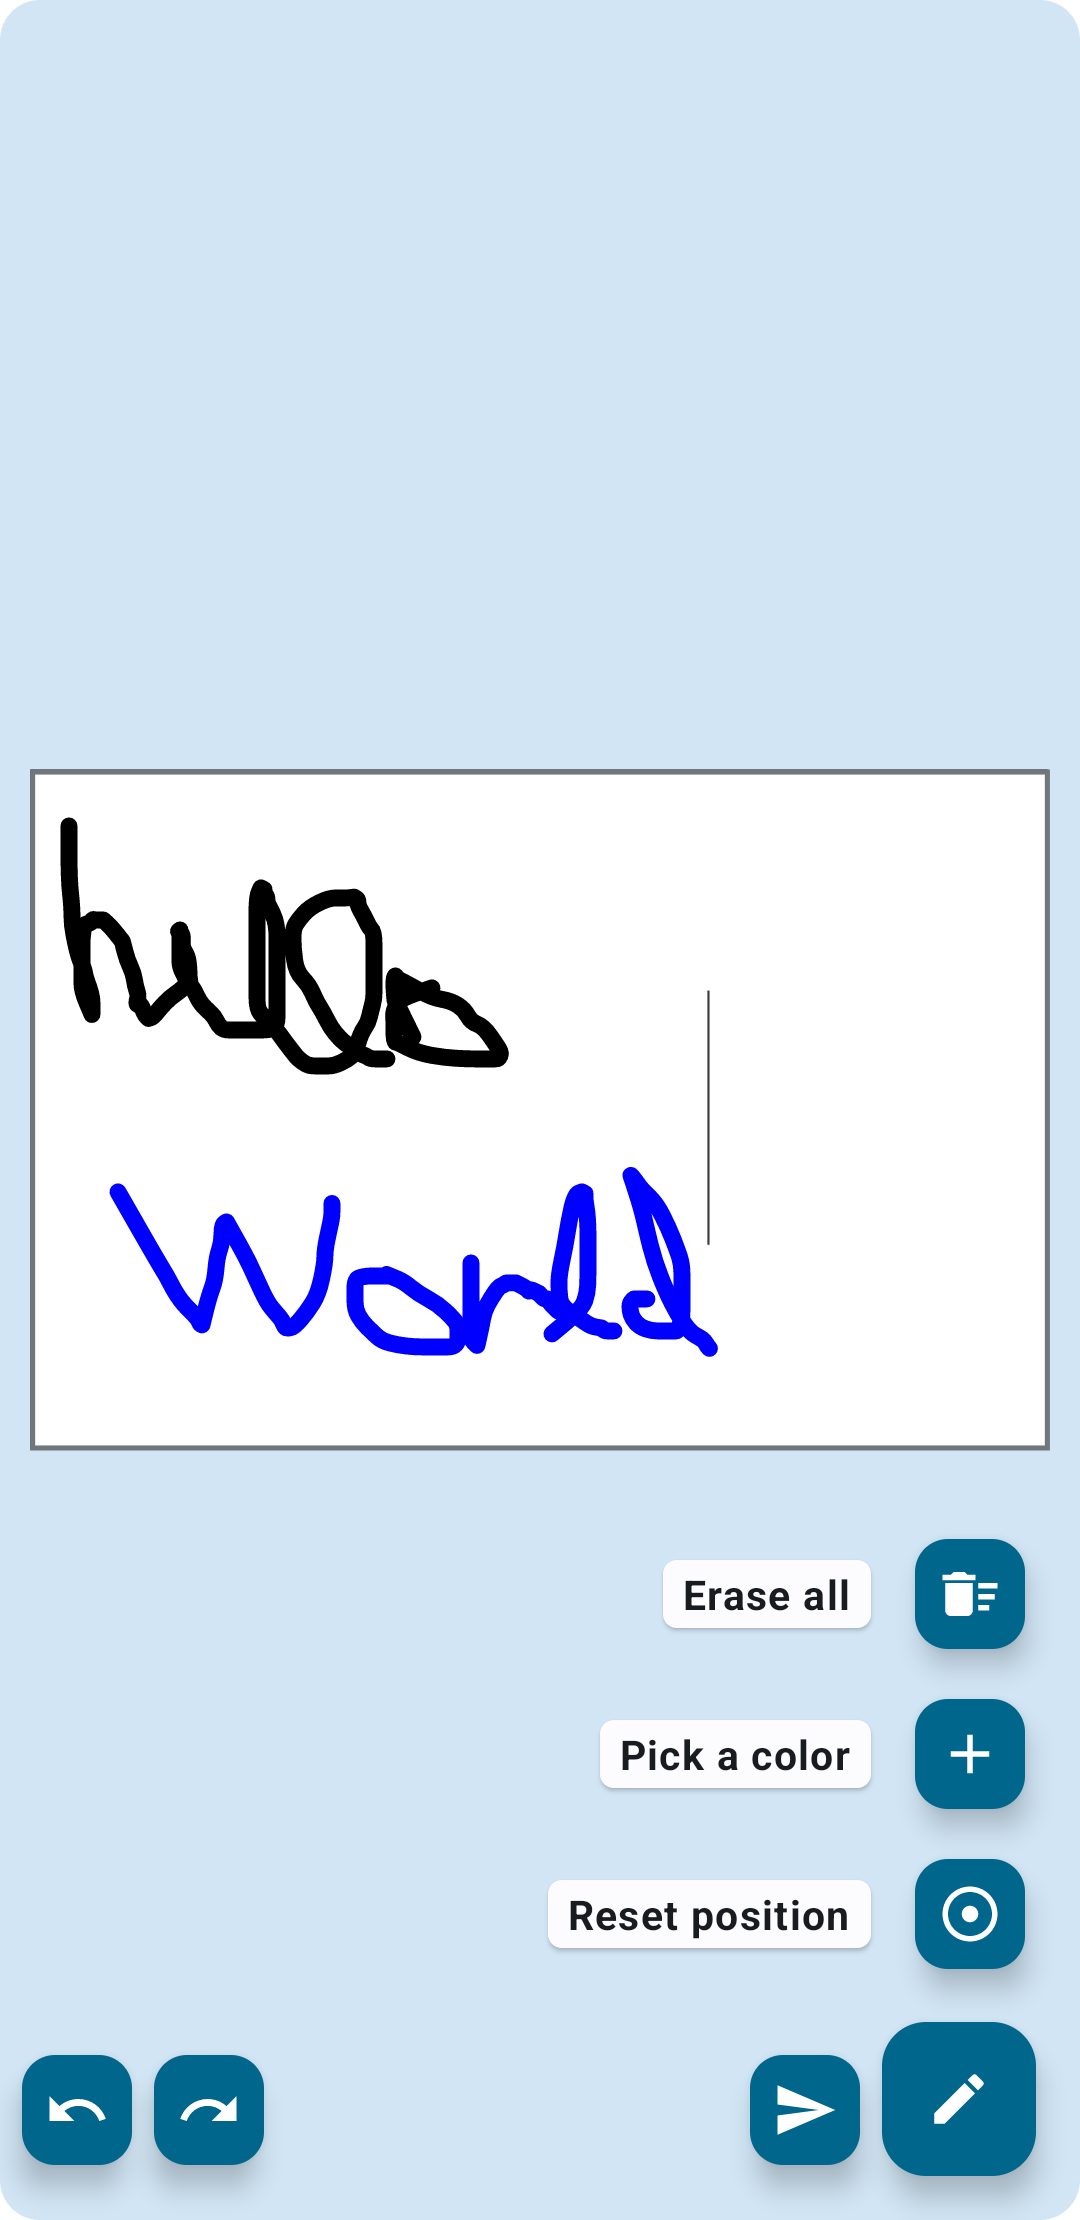
\includegraphics[trim={0cm -3cm 0 -3cm}, width=0.4\textwidth]{./Chapter6/Figures/DrawActivity}
	\caption{Draw Activity}
	\label{fig:DA1}
\end{figure}


\subsection{View Postcard}
The View Postcard Activity provides users with a dedicated interface to view postcards. It offers the ability to save and perform HTR over a postcard. 
When saving a file the user is prompted to choose the quality (from 1 to 5) this will multiply the default width and height of the SVG by the chosen value. The postcard is saved in the images media folder.
This activity focuses on delivering a seamless and immersive experience for users to enjoy the postcard content.

Figures \ref{fig:VA}, \ref{fig:VA1} and \ref{fig:VA2} illustrate the implemented activity.

\begin{figure}[!ht]
	\centering
	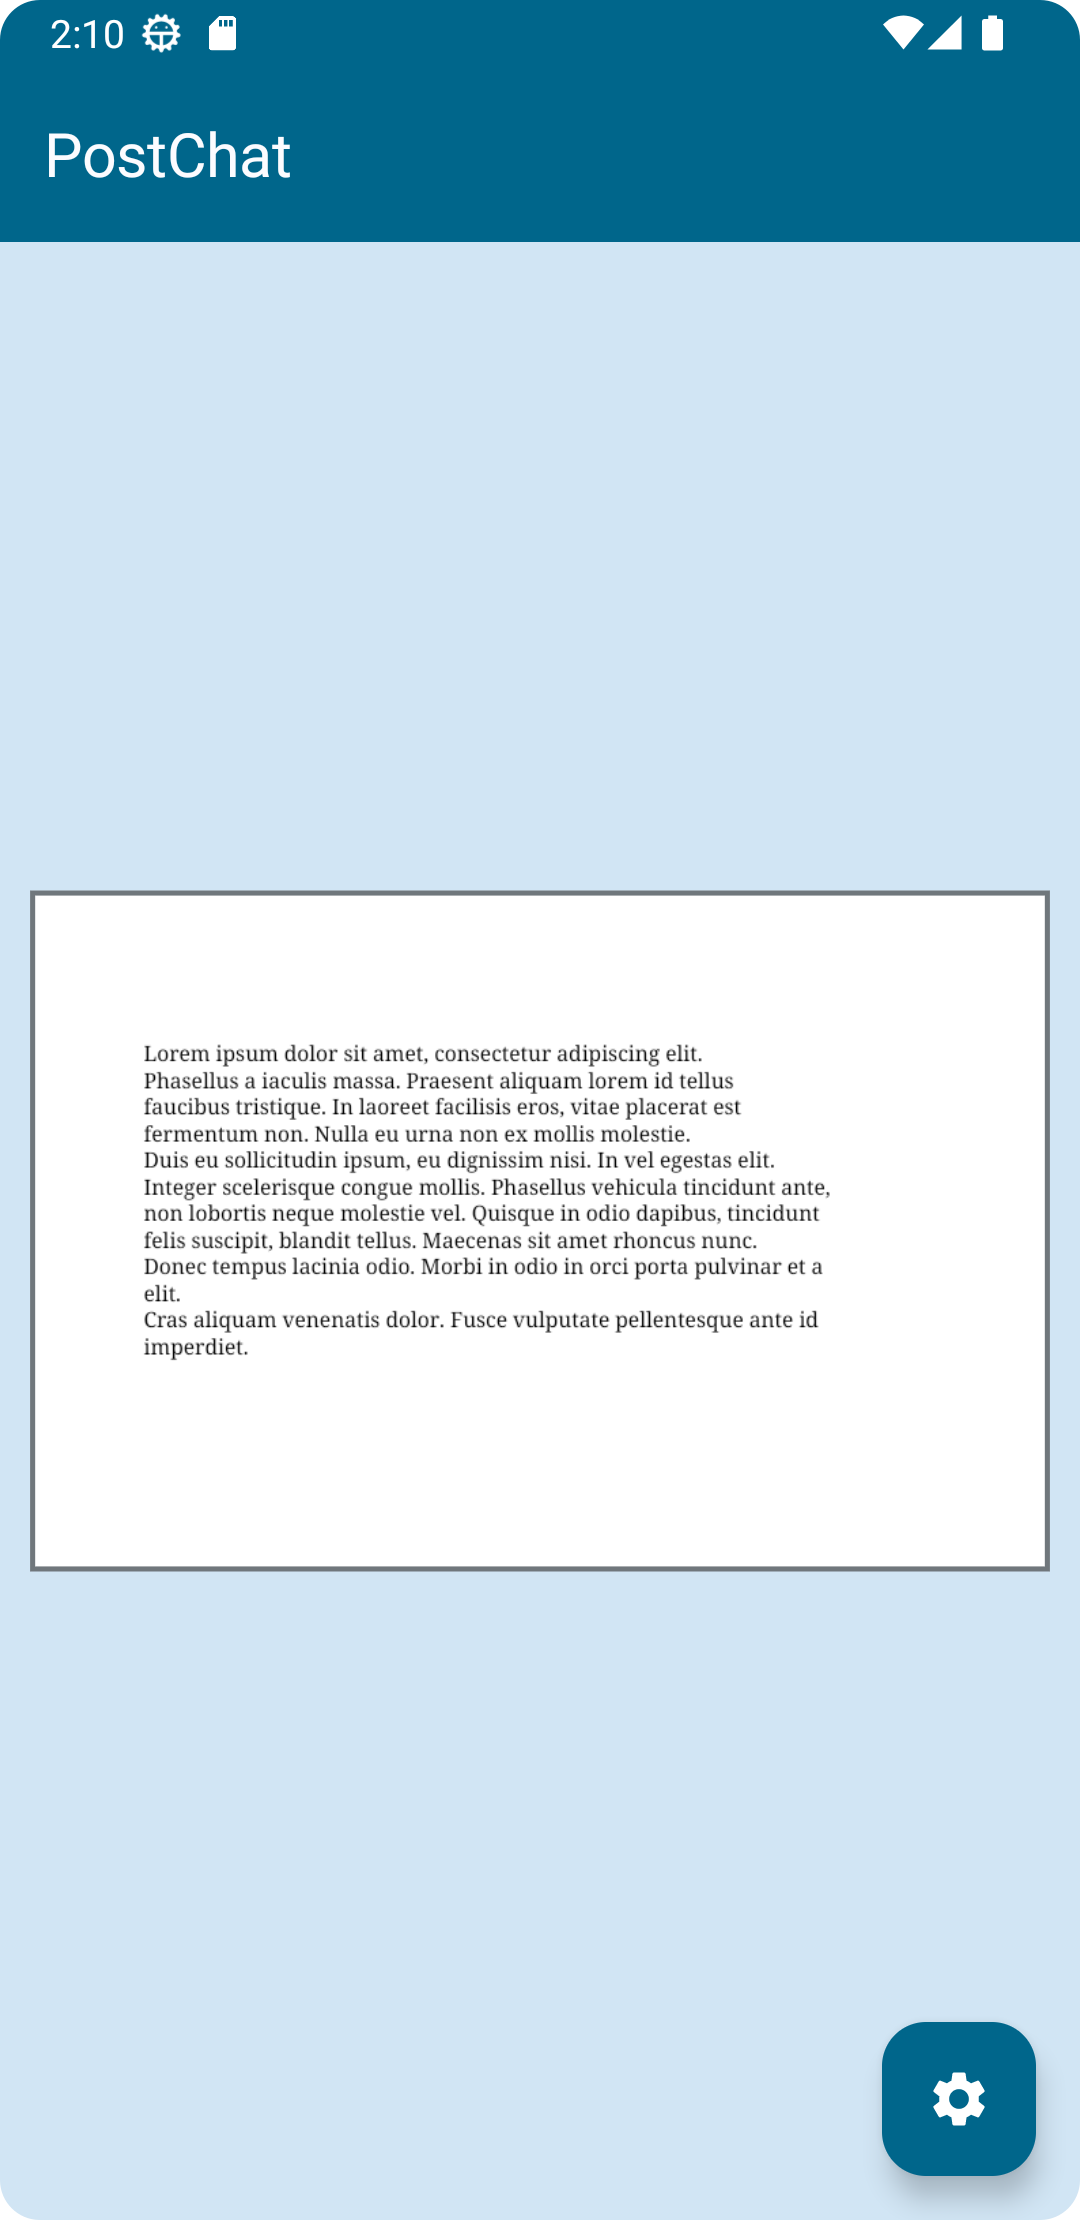
\includegraphics[trim={0cm -3cm 0 -3cm}, width=0.4\textwidth]{./Chapter6/Figures/PostcardActivity}
	\caption{Postcard View}
	\label{fig:VA}
\end{figure}


\begin{figure}[!ht]
	\centering
	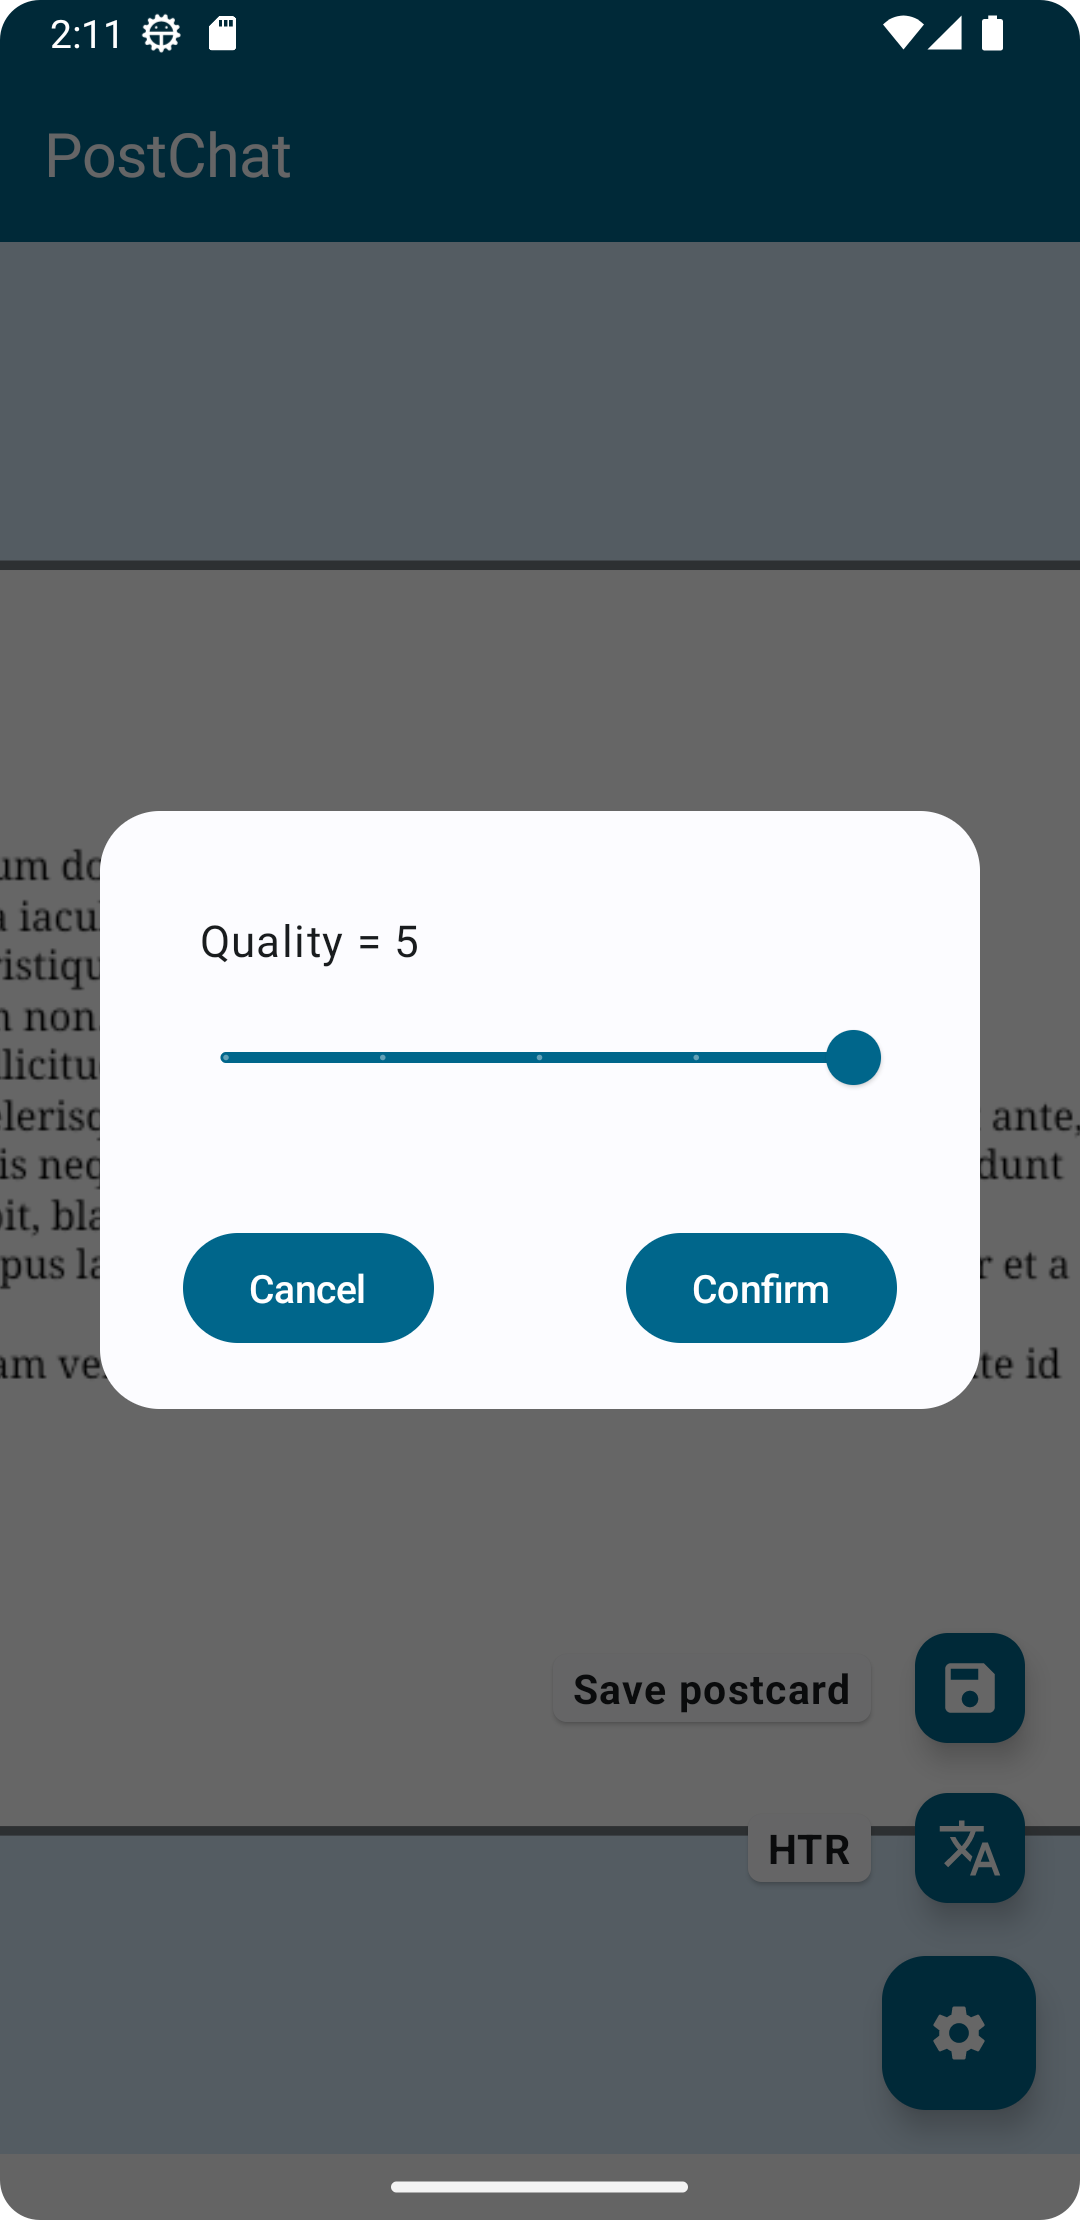
\includegraphics[trim={0cm -3cm 0 -3cm}, width=0.4\textwidth]{./Chapter6/Figures/PostcardActivitySave}
	\caption{Postcard save}
	\label{fig:VA1}
\end{figure}

\begin{figure}[!ht]
	\centering
	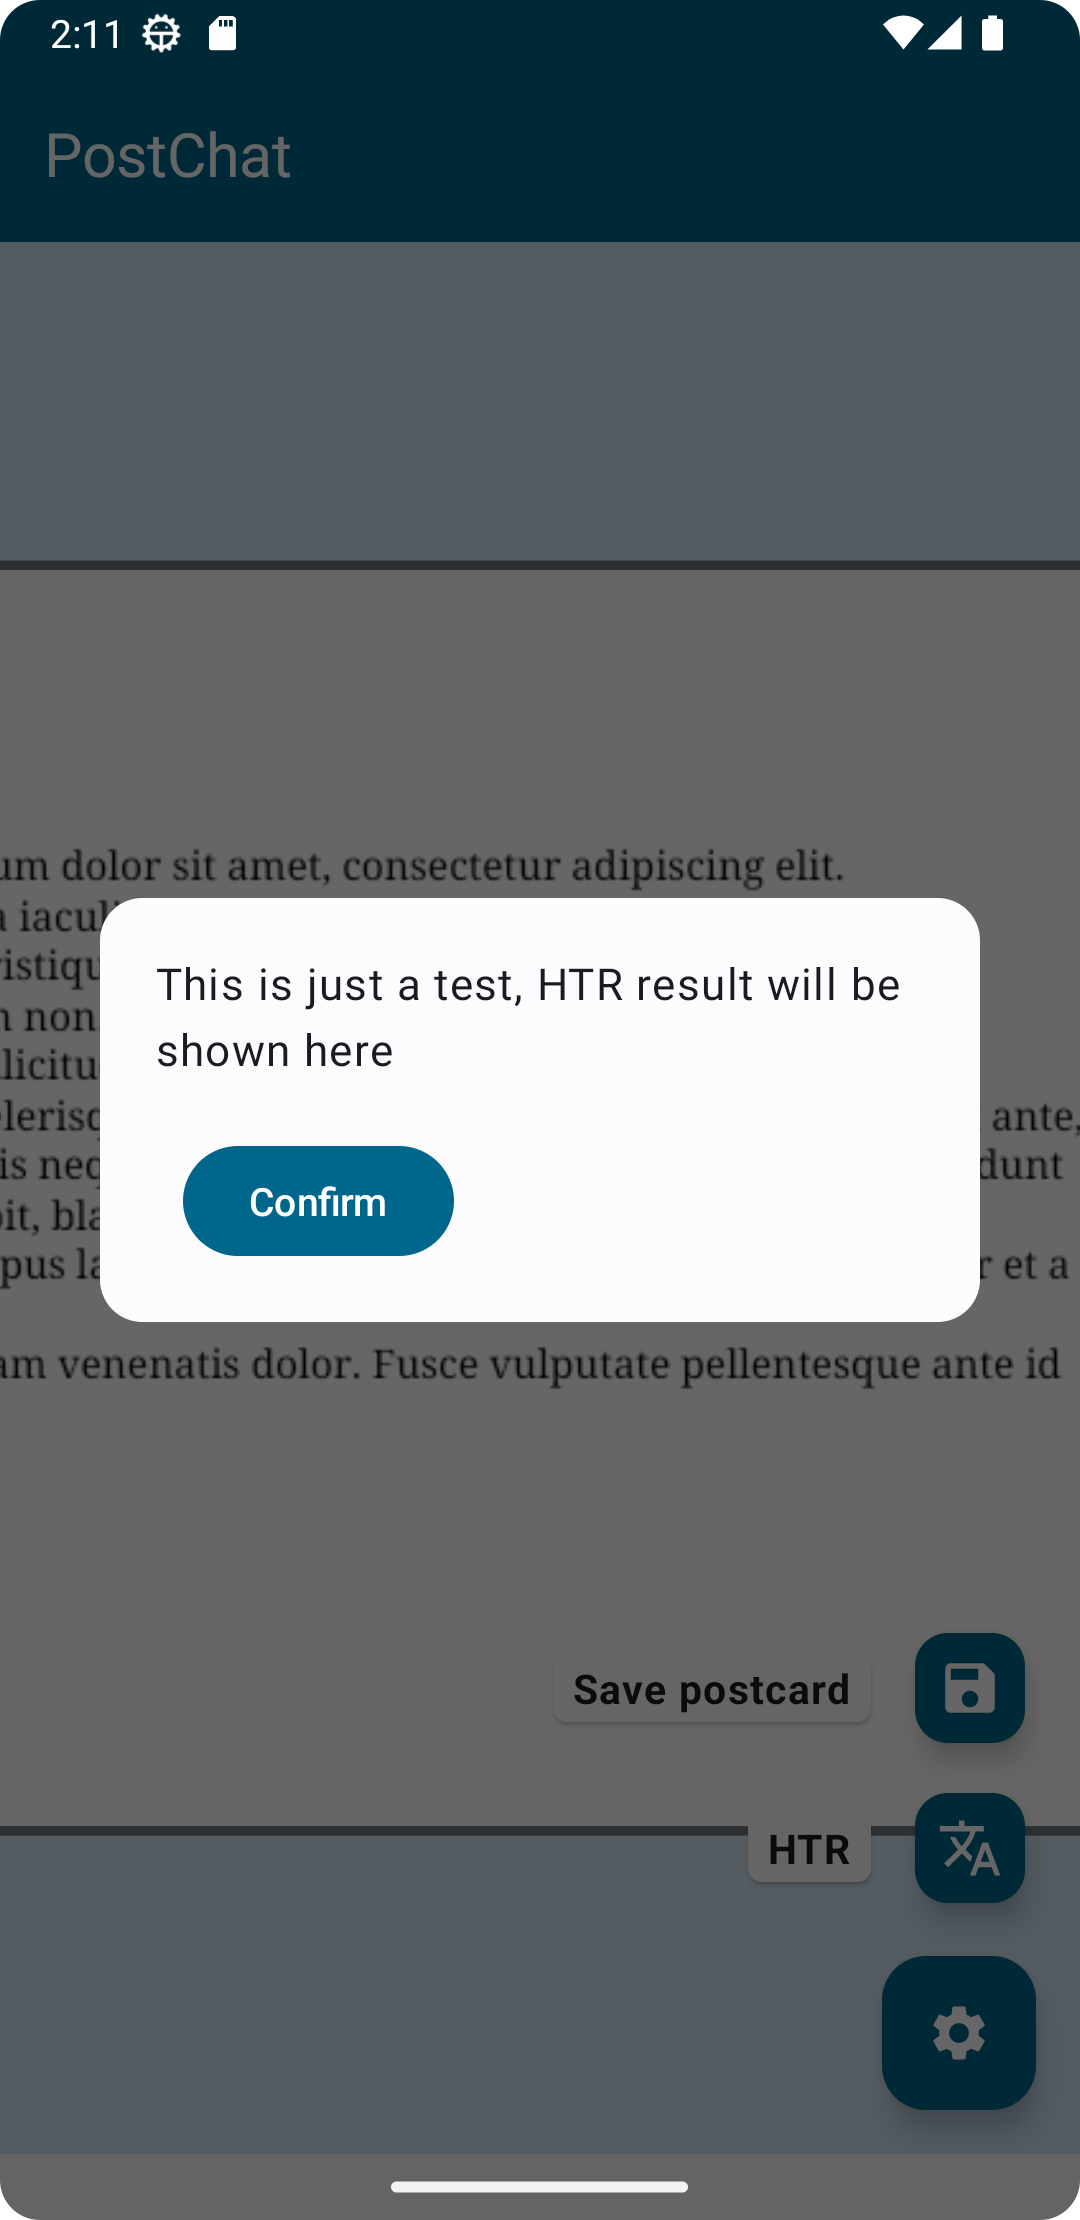
\includegraphics[trim={0cm -3cm 0 -3cm}, width=0.4\textwidth]{./Chapter6/Figures/PostcardActivityHTR}
	\caption{Postcard perform HTR}
	\label{fig:VA2}
\end{figure}


\subsection{Settings and Information}
The settings activity plays a major role in debugging but it is not limited to just that.

In this activity a user can delete its account or logout from the service.
Other settings are just for data visualization by the programmer and should be treated as so. They offer no utility for the final consumer and will be hidden from the same when ready for production.

There is a icon in the top right of the corner that leads to the activity containing information about the program and team behind it.

Figures \ref{fig:SIA} and \ref{fig:SIA1} illustrate the implemented activities.

\begin{figure}[!ht]
	\centering
	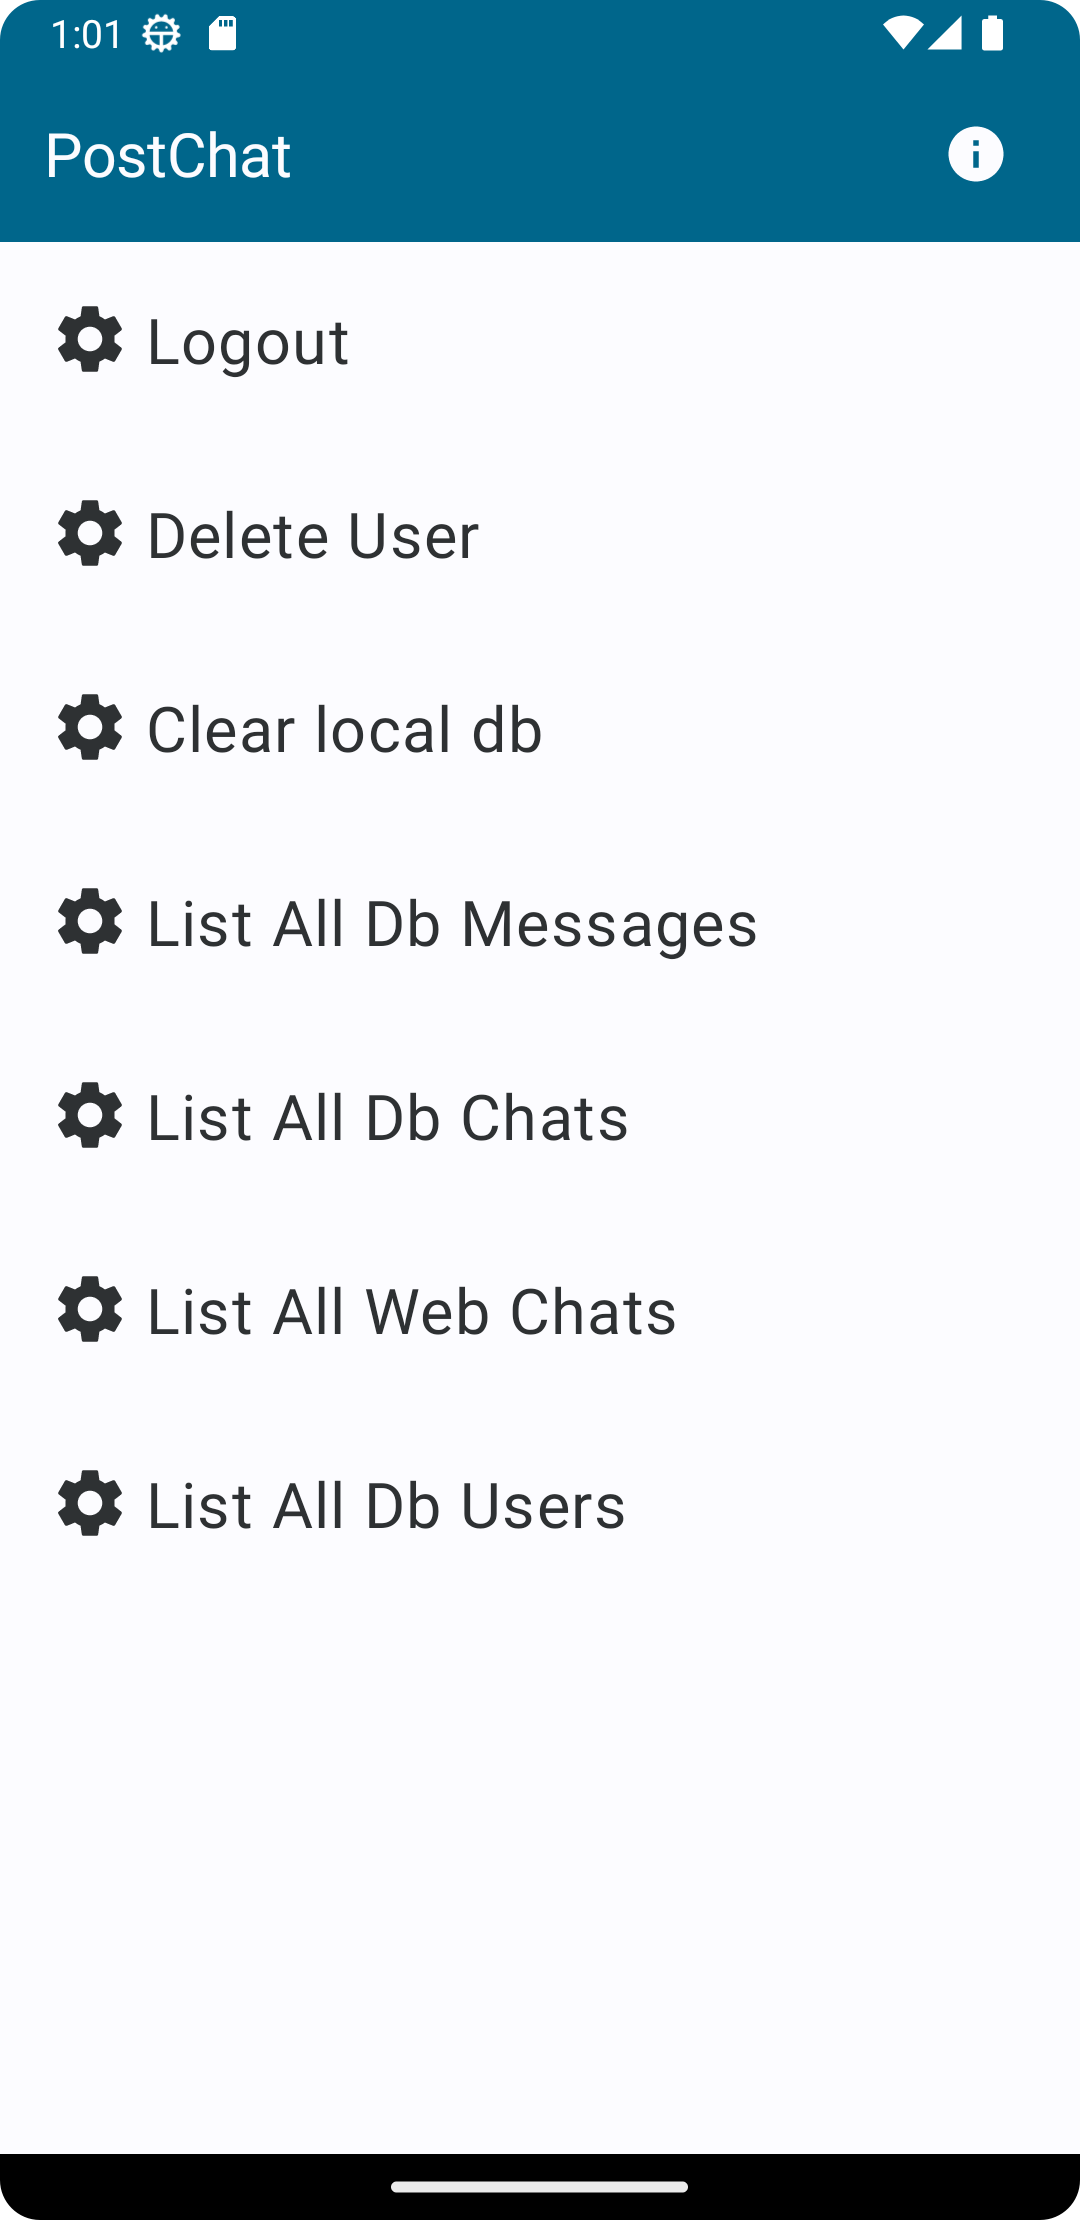
\includegraphics[trim={0cm -3cm 0 -3cm}, width=0.4\textwidth]{./Chapter6/Figures/SettingsActivity}
	\caption{Settings activity}
	\label{fig:SAI}
\end{figure}


\begin{figure}[!ht]
	\centering
	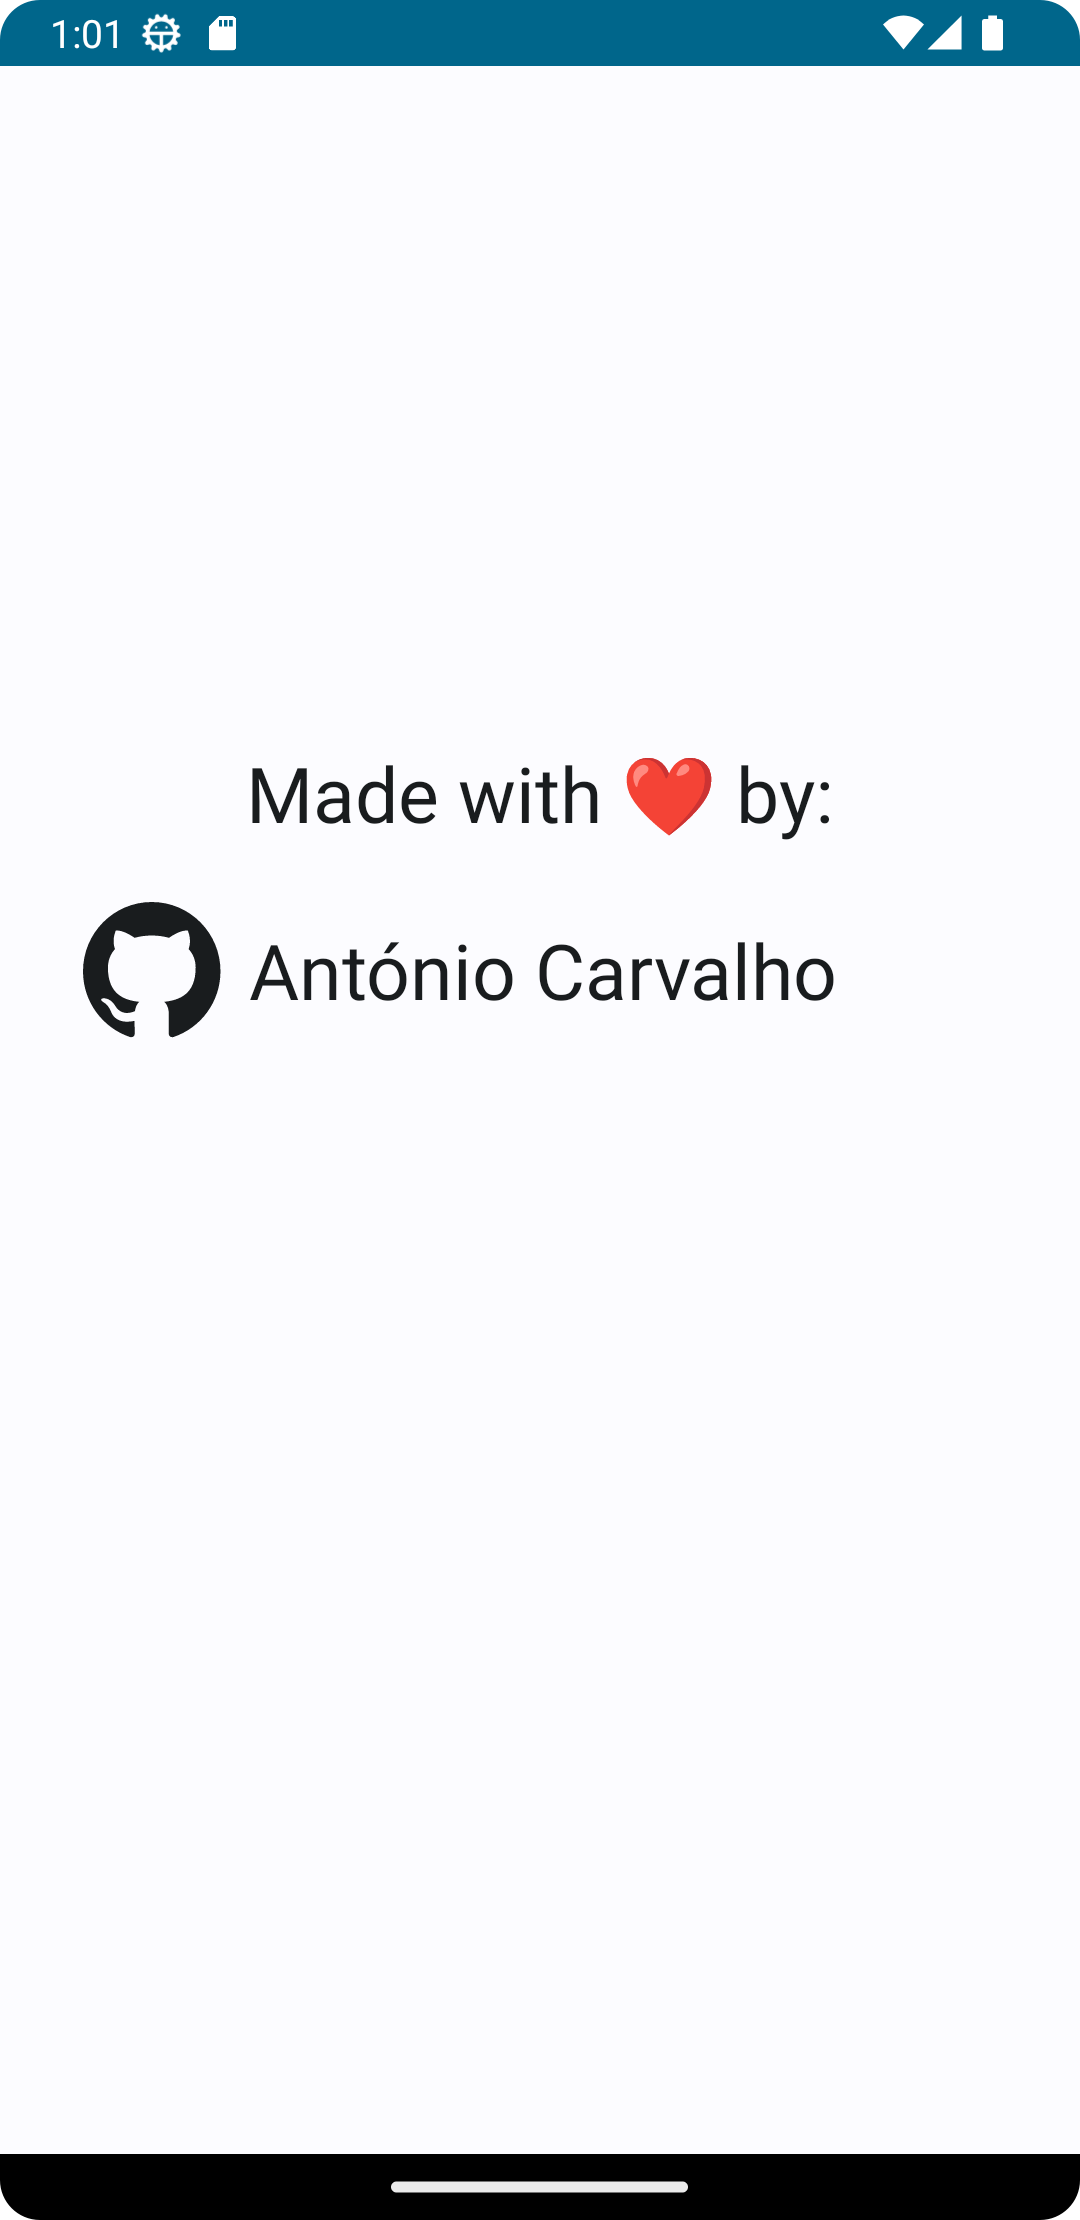
\includegraphics[trim={0cm -3cm 0 -3cm}, width=0.4\textwidth]{./Chapter6/Figures/InfoActivity}
	\caption{Information activity}
	\label{fig:SAI1}
\end{figure}





%/////////////////////////////////////////////////////////////
%   Chapter 8
%
%   Conclusions and Future Work
%
%/////////////////////////////////////////////////////////////
\chapter{Conclusions and Future Work} 
\label{ch:Chapter8}
\vfill \minitoc \newpage

In this project, we have developed a comprehensive application that integrates various components, including a Handwritten Text Recognition (HTR) model, a web API, and an Android application frontend. The aim of the project was to provide users with a seamless and efficient solution for communicating using digital postcards and to expand our knowledge of the AI world as we go.

In terms of future work, there are several areas that can be further improved and expanded upon. Bug fixes and performance optimizations should be prioritized to ensure the stability and efficiency of the application. Additionally, further testing, including unit testing and integration testing, should be conducted to identify and address any potential issues.

Furthermore, the application can be enhanced by implementing additional functionalities and features. This may include integrating social sharing capabilities, enabling users to share their postcards on social media platforms.

Overall, this project has demonstrated the successful integration of Handwritten Text Recognition (HTR) technology, a web API, and an Android application frontend to create a comprehensive postcard sending system. By leveraging these technologies, users can easily personalize and send their handwritten postcards, making the process more efficient and convenient. With continued development and refinement, the application has the potential to provide users with a seamless and enjoyable communication process.




% ///////////////////////////////////////////////////////
% Configuracao do header para apendices e referencias
% ///////////////////////////////////////////////////////

% Formato da pagina esquerda (par): <Pagina><Capitulo nr Nome>
\fancyhead[LE]{\small\thepage\hspace{3em}\nouppercase{\small\leftmark}}
\fancyhead[RE,LO]{}
% Formato da pagina direita (impar): <Numero da Seccao> <Nome da seccao> <Pagina>
\fancyhead[RO]{\nouppercase{\small\rightmark}\hspace{3em}\small\thepage}


%% The Appendices part is started with the command \appendix;
%% appendix sections are then done as normal sections
%% \appendix

%% \section{}
%% \label{}

%\appendix
%
%\renewcommand\thesection{\Alph{section}}

\renewcommand\chaptername{Appendix}

% Use:
%\appendix
%
% Or use:
\begin{appendices}

%\adjustmtc

%/////////////////////////////////////////////////////////////
%   Appendix A
% 
%   
%
%/////////////////////////////////////////////////////////////
\chapter{Other Definitions}
\label{app:AppendixA}
%\vfill \minitoc \newpage



\section{Technologies}
\begin{itemize}
	\item Spring Boot and MVC - Open Source Framework for Web Applications;
	\item JVM - Java Virtual Machine;
    \item Tensorflow - TensorFlow is a framework to create machine learning models for desktop, mobile, web, and cloud.
	\item Libphonenumber - Library to validate phone number format;
	\item Jetpack Compose - Android’s recommended toolkit for building native UI;
	\item Kotlin - Programming Language that extends Java base language;
\end{itemize}
	


%/////////////////////////////////////////////////////////////
%   Appendix B
% 
%   
%
%/////////////////////////////////////////////////////////////
%\chapter{Running times}
\label{app:AppendixB}
%\vfill \minitoc \newpage




%/////////////////////////////////////////////////////////////
%   Appendix C
% 
%   
%
%/////////////////////////////////////////////////////////////
%\chapter{Developed Software}
\label{app:AppendixC}
%\vfill \minitoc \newpage




\end{appendices}


% -------------------------------------------------------------
%   Bibliography
% -------------------------------------------------------------
%% Numbered
%\bibliographystyle{elsarticle-num} % Elsevier template (See Elsevier sample file)

%% APA style
\bibliographystyle{model5-names}

\bibliography{References/References}


\end{document}


